\documentclass[a4paper]{jreport}
\newcommand{\version}{5.0.1}

\title{{\vspace{2cm}{\Large Version \version} }}
\author{\Large Team SCALE\\ UGC working group}
\date{\today}


\usepackage[dvipdfmx]{graphicx}
\usepackage[dvipdfmx]{hyperref}
\usepackage{amsmath}
\usepackage{ascmac}
\usepackage[round]{natbib}
\usepackage{tabularx}
\usepackage{color}
\usepackage{colortbl}
\usepackage{fancybox}
\usepackage{url}
\usepackage{pxjahyper}
\hypersetup{% options for hyperref
 bookmarksopen=true,
 colorlinks=true,
 linkcolor=red,
 citecolor=cyan,
 urlcolor=cyan,
}
%\setlength{\textwidth}{42zw}
%\setlength{\textheight}{40\baselineskip}
\usepackage[top=30mm,bottom=35mm,left=30mm,right=30mm]{geometry}
\usepackage{wallpaper}
%\renewcommand{\thefootnote}{\fnsymbol{footnote}}
\renewcommand{\thefootnote}{*\arabic{footnote})}

\begin{document}
\CenterWallPaper{1.0}{figure/title_wallpaper.eps}
\maketitle
\ClearWallPaper
\ULCornerWallPaper{.1}{figure/scale_logo_final_ULWB.eps}
\tableofcontents

\chapter{概要}
\label{sec:overview}

%==============================================================%

本書は初めて領域気象気候モデル {\scalerm}
を利用する人に向けた解説書である。
気象気候ライブラリー{\scalelib}  version \version に対応した説明を記載する。
\scalelib の現バージョンには、領域モデル\scalerm と全球モデル\scalegm が含まれる。
本版では、\scalerm の使い方についてのみ詳しく述べる。
\scalegm については、次版で詳しく記載される予定である。
%\scalerm の使い方を通して、\scalelib を他のモデルからの呼び出す方法を
%習得することも可能です。

本書の構成は次の通りです。
第\ref{part:overview}部では SCALE の概要、
第\ref{part:install}部では必要な環境とインストール方法について説明する。
続いて、第\ref{chap:tutorial_ideal}章では理想実験、第\ref{chap:tutorial_real}章では現実大気実験を例にして、\scalerm の基本的な操作方法を説明する。
これらの章はひと繋がりのチュートリアルとなっており、
\scalerm を初めて使うユーザは一通り通読することを推奨する。
第\ref{part:basic_usel}部と第\ref{part:advance_use}部では、
モデルの設定の変更方法を記載し、また利用できるデータ形式やツールを説明する。
これらの各章は基本的にその中で閉じているので、辞書として用いることができる。

%%%
本書中の不明点やお気づきの点がございましたら、SCALE user's メーリングリスト\\
 \verb|scale-users@ml.riken.jp|までご連絡ください。



\section{\scalelib とは?} \label{subsec:scale_feature}
%--------------------------------------------------------------%

{\scalelib} (Scalable Computing for Advanced Library and Environment)は、
気候研究や天気予報を容易に様々な計算機上で行うためのソフトウェア・ライブラリである。
本ライブラリは、前処理からシミュレーション、後処理、解析に至るまで全ての過程を網羅し、
下記に挙げる長所を持つ。
\begin{itemize}
\item \scalelib は、「BSD-2ライセンス」のもとオープンソースソフトウェア
として提供している。
商用、非商用に関わらず自由な利用、改変、再配布が可能である。
\item \scalelib には、{\scalerm} (SCALE-Regional Model)
%SCALE-GM(SCALE-Global Model)
という領域モデルが含まれる。
\item \scalelib には、次節で説明するように様々なスキームが用意されている。
ユーザーが行いたい実験に合わせて適宜選択できる。
\item \scalelib では、\scalerm だけでなく他の数値モデルでも呼び出せる
物理過程のフレームワークを提供している。
\end{itemize}

ライセンスの詳細は、トップディレクトリ直下の\texttt{scale-\version/LICENSE}のファイルに記述されている。
\scalelib の使用前に一読されたい。
また、\scalelib のWebページ(\url{http://scale.aics.riken.jp/})にもソフトウェアの説明が記載されているので必要に応じて参照されたい。

本節では、\scalelib の思想や実際のモデルとの関係について説明する。
\scalerm の実行とは直接的には関係しないため、必要なければ読み飛ばしても構わない。

\Item{\scalelib のライブラリとモデルの関係について}

\begin{figure}[htb]
\begin{center}
  \includegraphics[width=0.9\hsize]{./figure/library_jp.eps}\\
  \caption{\scalelib のねらい}
  \label{fig:scale}
\end{center}
\end{figure}

\scalelib は幾つかの外部共同研究者と共に理化学研究所(RIKEN)で開発され、
その改良と拡張が継続的に行われている。
図 \ref{fig:scale}に\scalelib の思想の概念図を示す。
この図に示されるように、\scalelib は様々な問題に対応することを目指している。
\scalelib は、小型PCクラスターから次世代のスーパーコンピュータに至るまで様々な計算環境で広く用いられる事を念頭に開発されている。
この目的のため、気候・気象科学を専門とする科学者と計算機科学を専門とする科学者が
共同で開発している。

\scalerm は \scalelib ライブラリを大いに利用した数値モデルの一つであり、
図\ref{fig:scale-rm}に示すように \scalelib のパッケージに含まれる。
\scalelib は、並列プロセスの管理、ファイルの入出力、プロセス間の通信、格子情報の設定を行う。
また、\scalelib は、大気の流れのソルバ(力学コア)や雲微物理や大気放射等の物理過程も提供する。
その一方で、\scalerm は\scalelib が提供する機能を組み合わせることで構築されている。
\scalerm 自体は、大気の状態の入力データを予報変数として読み込んで保持し、
\scalelib の各コンポーネントを適宜呼び出すことで時間発展を計算する。
ユーザは行いたい実験に応じて、各コンポーネントのスキームを選択できる。

\begin{figure}[hbt]
\begin{center}
  \includegraphics[width=0.9\hsize]{./figure/scale_jp.eps}\\
  \caption{{\scalelib}ライブラリと{\scalerm}(モデル)の関係}
  \label{fig:scale-rm}
\end{center}
\end{figure}



\section{\scalerm の構成}  \label{subsec:sturcture_scale_rm}
%--------------------------------------------------------------%
\scalelib に含まれる全てのコンポーネント中の全てのスキームを、
\scalerm において利用できる。
コンポーネントは3つの部分(フレームワーク、力学コア、物理過程)に分類される。
以下に、\scalerm の現版に実装済みである、様々なスキームを含むコンポーネントを列挙する%
\footnote{
モデルの構成や離散化法の詳細は、
\citet{scale_2015}、\citet{satoy_2015b}、
\citet{nishizawa_2015}を参照されたい。
}。
\\

{\bf フレームワーク}
\begin{itemize}
 \item 実距離に基づいた3次元カーテシアン格子系
 \item MPI通信を用いた2次元領域分割
 \item 各種地図投影法
 \item 領域ネスティングシステム(1 way:親領域$\to$子領域へデータ転送)
   \begin{itemize}
    \item オンライン・ネスティング: 複数ドメインの計算を同時に実行
    \item オフライン・ネスティング:外側ドメインの計算終了後に、その結果を用いて内側ドメインの計算を実行
   \end{itemize}
 \item 複数事例一括実行システム(バルクジョブシステム)
 \item CF 規約\footnote{\url{http://cfconventions.org/}}に基づく \netcdf ファイル I/O
   \begin{itemize}
   \item {\netcdf}3 または {\netcdf}4 形式を選択
   \end{itemize}
 \item 理想実験のための初期値データ生成
 \item 外部データから標高・土地利用区分データを作成
 \item 外部データから初期値・境界値データを作成
   \begin{itemize}
    \item
      WRF-ARW\footnote{\url{http://www.wrf-model.org/}}、
%      NICAM\footnote{\url{http://nicam.jp/}}、
      \grads \footnote{\url{http://cola.gmu.edu/grads/}}形式での入力に対応
   \end{itemize}
\end{itemize}

{\bf 力学コア}
\begin{itemize}
 \item 支配方程式系: 3次元完全圧縮非静力学方程式系
 \item 空間離散化: 有限体積法
    \begin{itemize}
      \item 2次, 4次, 6次中央差分
      \item 3次, 5次風上差分
    \end{itemize}
 \item 時間離散化: 「完全陽解法」または「水平陽解法-鉛直陰解法」から選択
    \begin{itemize}
      \item Heun型3次ルンゲ・クッタスキーム
      \item \citet{Wicker_2002}の3段ルンゲ・クッタスキーム
      \item 4次ルンゲ・クッタスキーム
    \end{itemize}
 \item 非負保証:
    \begin{itemize}
      \item フラックス修正法 \citep[Flux Corrected Transport, FCT; ][]{zalesak_1979}
      \item \citet{Koren_1993}フィルター  (3次風上差分スキーム使用時のみ)
    \end{itemize}
 \item 数値フィルタ: 4次超粘性・拡散
 \item 地形: 地形に沿った座標系を用いて表現
\end{itemize}

{\bf 物理過程}
\begin{itemize}
 \item 乱流過程: 以下から選択可能
   \begin{itemize}
    \item \citet{smagorinsky_1963} \& \citet{lilly_1962}型のサブグリッドスケール乱流モデル (\citet{Brown_etal_1994}と\citet{Scotti_1993}による補正)
    \item \citet{Deardorff_1980} サブグリッドスケール乱流モデル
    \item \citet{my_1982,nakanishi_2004}によるlevel 2.5境界層乱流パラメタリゼーション
   \end{itemize}
 \item 雲微物理: 以下から選択可能
   \begin{itemize}
    \item \citet{kessler_1969}による3-class 1モーメントバルクモデル
    \item \citet{tomita_2008}による6-class 1モーメントバルクモデル
    \item \citet{sn_2014}による6-class 2モーメントバルクモデル
    \item \citet{suzuki_etal_2010}によるビン法モデル
   \end{itemize}
 \item 放射過程: \citet{sekiguchi_2008}による相関k分布法ブロードバンド大気放射伝達モデル
 \item 地表面モデル
  \begin{itemize}
   \item 陸面モデル: 熱拡散・バケツモデル
   \item 海洋モデル: 以下から選択可能
   \begin{itemize}
     \item 初期値固定
     \item 外部データ入力
     \item スラブモデル
   \end{itemize}
   \item 都市モデル: \citet{kusaka_2001}による単層キャノピーモデル
   \item バルク交換係数(陸面および海面): 以下から選択可能
   \begin{itemize}
     \item \citet{beljaars_1991,wilson_2001}による普遍関数によるバルク法
     \item \citet{uno_1995}によるLouis 型バルク法
   \end{itemize}
  \end{itemize}
\end{itemize}


This document assumes an execution in the shell ``bash'' on some Unix system.
If your environment is different, replace the commands
by the relevant commands suitable for your environment.
Unless there is a particular remark, this documentation obeys the following notation:

The command-line symbol for execution is expressed by \verb|$| or \verb|#|.
The difference between the two notations is
in the permission levels of program execution, as shown below:
\begin{verbatim}
 #        <- command by root permission
 $        <- command by user permission
\end{verbatim}

A description enclosed in a rectangle expresses a message generated by the command line, as shown below.
\msgbox{
 -- -- -- -- command-line message\\
 -- -- -- -- -- -- -- -- command-line message\\
 -- -- -- -- -- -- -- -- -- -- -- -- command-line message\\
}

On the other hand, a description enclosed in a rounded rectangle shows a part of configuration file including namelists, which can be edited as needed.
\editbox{
 -- -- -- -- description in a file\\
 -- -- -- -- -- -- -- -- description in a file\\
 -- -- -- -- -- -- -- -- -- -- -- -- description in a file\\
}

In this documentation, the FORTRAN namelist and its items are denoted by
\namelist{namelist} and \nmitem{item_of_namelist}, respectively.



\chapter{インストール}
\label{sec:install}
\section{Installation of SCALE-LES}
%####################################################################################

本章では,日本域を対象とした現実大気再現実験のチュートリアルを通して,
SCALE-LESモデルを実行する一連の作業を説明する.
SCALEライブラリのインストールに必要な環境、ライブラリのインストール方法については,
\ref{sec:req_env}節とAppendix \ref{sec:env_setting}を参照して
事前にインストールしておく必要がある.
\ref{sec:source_code}以降のチュートリアルは,それらのライブラリ環境が
インストールされていることを想定して進める.


\subsection{Required Environment}
\label{sec:req_env}
%====================================================================================

\begin{itemize}
  \item {\bf 計算機環境} : Unix互換OS (Mac OS Xを含む)が動作する環境.
        マルチコアCPU環境以上を推奨する.
        実験サイズによるが4GB以上のメモリがインストールされているマシン環境が好ましい.
  \item {\bf OS} : Linux OS(Fedora, CentOS, SUSE等),Mac OS X.ここではLinux (CentOS6)を使用して説明する.
  \item {\bf コンパイラ} : Fortran 2003をサポートするC,Fortranコンパイラを必要とする.
        GNU 4.6.x以上,Intel compiler 2012以上を推奨する.ここでは,gcc/gfortranを使用して説明する.
  \item {\bf MPIライブラリ} : MPICH2, OpenMPI, Intel MPI等をサポートする.ここではopenMPIを使用して説明する.
  \item {\bf netcdf3 もしくは HDF5/netcdf4} : gzip, szipをサポートするHDF5,
        およびそのHDF5をサポートするnetcdf4を必要とする.
        ただし,netcdf3の環境下ではscaleライブラリが提供する全ての機能をサポートできない可能性がある.
  \item {\bf 描画環境(非必須)} : Dennou Club提供のRuby DCL/GPhysに含まれるgpviewがあると
        計算結果を簡単にチェックできる.チュートリアルではgpviewを使用する.
        それ以外に,netcdfからGrADS用にフォーマットを変換するためのpostprocess(\verb|netcdf2grads_h|)も用意している.
  \item SCALEは演算性能評価のためにPAPIライブラリを使用が可能.
        PAPIライブラリがインストールされている環境下では,
        以下で説明するconfigureファイルの編集によってPAPIを適用することができます.
\end{itemize}


\subsection{Building the source code} \label{sec:source_code}
%====================================================================================

\subsubsection{ソースコードの入手}
%-----------------------------------------------------------------------------------

安定版ソースコードは,\url{http://scale.aics.riken.jp/ja/download/index.html}
よりダウンロードすることができる.
ソースコードのtarballファイルを展開すると
\begin{verbatim}
  scale/
\end{verbatim}
というディレクトリができる.

現実大気実験のシミュレーションを行う場合,SCALE本体に加えて境界値データが必要になる.
本チュートリアル用の気象場のデータ,日本領域の地形・土地利用のデータを\\
 \url{http://scale.aics.riken.jp/download/tutorial_data.tar.gz}\\
より入手し,チュートリアルの入力ファイル用ディレクトリ
\begin{verbatim}
  scale/scale-les/test/tutorial/data/
\end{verbatim}
の下に展開しておく.

以降の説明で\verb|${TOPDIR}|は,\verb|scale/scale-les/test/tutorial/|がある絶対PATHを指す.

\begin{verbatim}
  ${TOPDIR}/data/tutorial_data/input_atom/    <- 気象場データ
  ${TOPDIR}/data/tutorial_data/input_topo/    <- 地形データ
  ${TOPDIR}/data/tutorial_data/input_landuse/ <- 土地利用データ
\end{verbatim}
\verb|tutorial_data/|には,本チュートリアルに必要な最低限のデータのみが納めされているため,
その他の設定で実験を行う場合には別途,気象場,地形,および土地利用データが必要となる.


\subsubsection{configure ファイルと環境変数の設定}
%-----------------------------------------------------------------------------------

\verb|scale/sysdep/|内にいくつかのコンフィグファイル(\verb|Makedef.***|)が準備されている.
これらの中から自分の環境にあったものを設定する.
ここでは,OSはLinux,コンパイラはgcc/gfortran,およびopenMPIを使用するため,
\verb|"Makedef.Linux64-gnu-ompi"|が対応するファイルとなる.
自分の環境に合うものがなければ既存ファイルをベースにして作成する.

常にこのコンフィグファイルをしようするために、
\verb|Makedef.***|の\verb|"***"|の部分を、\verb|SCALE_SYS|という環境変数として設定し、
\verb|.bashrc|などのファイルに記述しておくと便利である.
さらに、SCALEをコンパイルするのに必要な外部ライブラリについても
下記のようにPATHを設定する.
ここでは,Appendix \ref{sec:env_setting}に従ったとして,
HDF5,netcdf4ともに\verb|/usr|の下にインストールされている場合の例を示す.

\begin{verbatim}
 $ export SCALE_SYS="Linux64-gnu-ompi"
 $ export HDF5="/usr"
 $ export NETCDF4="/usr"
\end{verbatim}


\subsubsection{コンパイル}
%-----------------------------------------------------------------------------------

下記のディレクトリに移動して,makeコマンドによってコンパイルを行う.
\begin{verbatim}
 $ cd ${TOPDIR}/bin
 $ make -j 4
\end{verbatim}
\verb|make|のあとの \verb|"-j 4"| は,並列コンパイルを指示するオプションで,
4並列コンパイルを行うことを指示している.
コンパイルを実行する環境によっては並列数を増やすこともできる.
このmakeによってSCALEライブラリ,およびSCALE-LESモデルのコンパイルが行われ,
結果として
\begin{verbatim}
 scale-les  scale-les_init  scale-les_pp
\end{verbatim}
の3つの実行ファイルが生成されていればコンパイルは成功である.\\


{\bf 注意点}
\begin{itemize}
\item SCALEライブラリは,scaleのTOPディレクトリ直下の
 \verb|scale/scalelib/|というディレクトリ内でコンパイルとアーカイブが行われ,
 \verb|".lib"|という名前の隠しディレクトリとして
 \verb|bin/|ディレクトリ内へコピーされている.
\item Debugモードでコンパイルしたい場合や,
 コンパイルオプションを変更したい場合は,
 \verb|Makedef.***|のファイルを編集してください.
\item 開発版ソースコードをコンパイルしている場合,
 一部のコンパイラバージョンにおいてコンパイルが正常に終了しないケースがあります.そのような場合はぜひSCALE開発チームまでご報告ください.
\end{itemize}


%####################################################################################



\chapter{チュートリアル: 理想実験}
\label{sec:tuto_ideal}
%%%%%%%%%%%%%%%%%%%%%%%%%%%%%%%%%%%%%%%%%%%%%%%%%%%%%%%%%%%%%%%%%%%%%%%%%%%%%%%%%%%%%%
%  File 31_ideal_exp.tex
%%%%%%%%%%%%%%%%%%%%%%%%%%%%%%%%%%%%%%%%%%%%%%%%%%%%%%%%%%%%%%%%%%%%%%%%%%%%%%%%%%%%%%


\section{内容の説明}
%====================================================================================

本章では、チュートリアルにおける1つめの実験として、SCALEを使った理想実験(Ideal case)の
実行方法を説明する。簡単な実験であるが、第\ref{sec:install}章で実行したSCALEのコンパイルが
正常に完了しているかどうかのチェックも含めてぜひ実施してもらいたい。

ここでは、SCALEのコンパイルが正常に終了し、
\begin{verbatim}
  scale-les/test/tutorial/bin
\end{verbatim}
に\verb|scale-les|、および\verb|scale-les_init|が生成されており、
\begin{verbatim}
  scale-les/util/netcdf2grads_h
\end{verbatim}
に\verb|net2g|が生成されているものとして説明を行う。
これらに加えて、本章のチュートリアルでは、描画ツールとしてGrADSを使用する。
GrADSの詳細やインストール方法については、Appendix \ref{sec:env_vis_tools}節を参照のこと。


ここで実行する理想実験は、「スコールライン」と呼ばれる積乱雲群を発生させる実験である。
実験設定の概要を表\ref{tab:setting_ideal}に示す。この実験は、積乱雲が発生する場合の
典型的な大気の成層構造を表現した鉛直プロファイルを与え、対流圏下層に置いた初期擾乱から
積乱雲が発達する様子を準2次元モデル実験する内容となっている。

\begin{table}[htb]
\begin{center}
\caption{チュートリアル理想実験の実験設定}
\begin{tabularx}{150mm}{|l|l|X|} \hline
 \rowcolor[gray]{0.9} 項目 & 設定内容 & 備考 \\ \hline
 水平格子間隔 & 東西:500 m、南北:1000 m & 東西-鉛直の面を切り取った準2次元実験である \\ \hline
 水平格子点数 & 東西:40、南北:2 & 東西-鉛直の面を切り取った準2次元実験である \\ \hline
 鉛直層数     & 97層(トップ:20 km)& 下層ほど細かい層間隔をとったストレッチ設定である \\ \hline
 側面境界条件 & 周期境界 & 東西、南北とも \\ \hline
 積分時間間隔 & 5 sec      & 雲微物理スキームは10 sec毎 \\ \hline
 積分期間     & 3,600 sec  & 720 steps \\ \hline
 データ出力間隔 & 300 sec  &  \\ \hline
 物理スキーム & 雲微物理モデルのみ使用 &
 6-class single moment bulk model (tomita 2006) \\ \hline
 初期鉛直プロファイル & GCSS Case1 squall-line &
 風のプロファイルは、Ooyama (2001)に基づいた鉛直シアを与える \\ \hline
 初期擾乱 & ウォームバブル & 水平半径4 km、
 鉛直半径3 kmの大きさを持つ最大プラス3Kの強度のウォームバブルを置く\\ \hline
\end{tabularx}
\label{tab:setting_ideal}
\end{center}
\end{table}

このチュートリアルを実行するには、最低でも2コア/4スレッドの演算コアを持つCPU、
512MB以上のメモリを搭載した計算機が必要である。本節の説明で使用した環境は次のとおりである。
\begin{itemize}
\item CPU: Intel Core i5 2410M 2.3GHz 2コア/4スレッド
\item Memory: DDR3-1333 4GB
\item OS: CentOS 6.6 x86-64, CentOS 7.1 x86-64, openSUSE 13.2 x86-64
\end{itemize}


\section{実行方法}
%====================================================================================

実行の流れとしては、下準備、初期値の作成、モデル本体の実行、
後処理、そして描画といった順番で作業を進める。

\subsection{下準備}
%------------------------------------------------------
チュートリアル理想実験は、\verb|scale-les/test/tutorial/ideal|の
ディレクトリにて実行するので、まずこのディレクトリに移動する。
\begin{verbatim}
  $ cd scale-les/test/tutorial/ideal
\end{verbatim}
次に、このディレクトリに対して、前章までに作成したSCALEの
実行バイナリの静的リンクを張る。
\begin{verbatim}
  $ ln -s ../bin/scale-les       ./
  $ ln -s ../bin/scale-les_init  ./
\end{verbatim}
``\verb|scale-les|''はモデル本体、``\verb|scale-les_init|''は
初期値・境界値作成ツールである。
もし、ここで説明するディレクトリとは異なる場所で実行している場合は、
リンクを張る時のディレクトリ指定に注意すること。

\subsection{初期値作成}
%------------------------------------------------------
ここでは、``\verb|scale-les_init|''を実行して初期値を作成する。``\verb|scale-les_init|''を
実行する際にはconfigファイルを与える。例えば、``\verb|init_R20kmDX500m.conf|''のファイルには、
表\ref{tab:setting_ideal}に対応した実験設定が書き込まれており、このconfigファイルの指示に
従って\verb|scale-les_init|は大気の成層構造を計算し、ウォームバブルを設置する。


SCALEの基本的な実行コマンドは下記のとおりである。
\begin{verbatim}
  $ mpirun  -n  [プロセス数]  [実行バイナリ名]  [configファイル]
\end{verbatim}
[プロセス数]の部分にはMPI並列で使用したいプロセス数を記述する。[実行バイナリ]には、
\verb|scale-les|や\verb|scale-les_init|が入る。そして、実験設定を記述したconfigファイルを
[configファイル]の部分に指定する。ここでは、\textcolor{red}{2つのMPIプロセス}を用いて実行する。
以降、これを「2-MPI並列」のように表現する。従って、\verb|init_R20kmDX500m.conf|を
configファイルとして与えて、2-MPI並列で\verb|scale-les_init|を実行する場合の
コマンドはつぎのようになる。
\begin{verbatim}
  $ mpirun  -n  2  ./scale-les_init  init_R20kmDX500m.conf
\end{verbatim}

\noindent 実行が成功した場合には、コマンドラインのメッセージは
下記のように表示される。\\

\noindent {\small {\gt
\fbox{
\begin{tabularx}{140mm}{l}
 *** Start Launch System for SCALE-LES\\
 TOTAL BULK JOB NUMBER   =    1\\
 PROCESS NUM of EACH JOB =     2\\
 TOTAL DOMAIN NUMBER     =    1\\
 Flag of ABORT ALL JOBS  =  F\\
 *** a single comunicator\\
 *** a single comunicator\\
\end{tabularx}
}}}\\

\noindent この実行によって、\\
``init\_LOG.pe000000''\\
``init\_00000000000.000.pe000000.nc''\\
``init\_00000000000.000.pe000000.nc''\\
の3つのファイルが、現在のディレクトリ下に作成されているはずである。``init\_LOG.pe000000''には、
コマンドラインには表示されない詳しい実行ログが記録されている。
実行が正常に終了している場合、このLOGファイルの最後に\\

\noindent {\small {\gt
\ovalbox{
\begin{tabularx}{140mm}{l}
 ++++++ Stop MPI\\
 *** Broadcast STOP signal\\
 *** MPI is peacefully finalized\\
\end{tabularx}
}}}\\

\noindent と記述される。

そして、``init\_00000000000.000.pe000000.nc''と``init\_00000000000.000.pe000001.nc''の
2つのファイルが初期値ファイルである。計算領域全体を2つのMPIプロセスで分割し担当するため、
2つのファイルが生成される。もし、4-MPI並列で実行すれば、4つの初期値ファイルが生成される。
これらのファイル名の末尾が``.nc''で終わるファイルはNetCDF形式のファイルであり、
Gphys/Ruby-DCLやncviewといったツールで直接読むことができる。


\subsection{モデル本体の実行}
%------------------------------------------------------
いよいよ、モデル本体を実行する。初期値作成のときと同じように2-MPI並列だが、
しかしconfigファイルは実行用の``\verb|run_R20kmDX500m.conf|''を指定する。
\begin{verbatim}
  $ mpirun  -n  2  ./scale-les  run_R20kmDX500m.conf
\end{verbatim}

本書の必要要件にあった計算機であれば、2分程度で計算が終わる。
\noindent この実行によって、\\
``LOG.pe000000''\\
``history.pe000000.nc''\\
``history.pe000000.nc''\\
``monitor.pe000000''\\
の4つのファイルが、現在のディレクトリ下に作成されているはずである。``LOG.pe000000''には、
コマンドラインには表示されない詳しい実行ログが記録されている。
実行が正常に終了している場合、このLOGファイルの最後に\\

\noindent {\small {\gt
\ovalbox{
\begin{tabularx}{140mm}{l}
 ++++++ Stop MPI\\
 *** Broadcast STOP signal\\
 *** MPI is peacefully finalized\\
\end{tabularx}
}}}\\

\noindent と記述される。

そして、``history.pe000000.nc''と``history.pe000001.nc''の2つのファイルが計算経過の
データが記録されたhistoryファイルである。このファイルもNetCDF形式のファイルであり、
2-MPI並列で実行したため、やはり2つのファイルが生成される。
``monitor.pe000000''は、計算中にモニタリングしている
物理変数の時間変化を記録したテキストファイルである。



\subsection{後処理と描画}
%------------------------------------------------------
ここでは、計算結果を描画するための後処理について説明する。本書のチュートリアルでは、
NetCDF形式の分散ファイルを1つのファイルにまとめ、ユーザーが解析しやすいDirect-Accessの
単純バイナリ形式(GrADS形式)に変換する方法を説明する。Gphys/Ruby-DCLを使うと
分割ファイルのまま直接描画することができるが、この方法については\ref{sec:quicklook}節を
参照してもらいたい。

まず、\ref{sec:source_net2g}節でコンパイルした後処理ツール``net2g''を、
現在のディレクトリへリンクを張る。
\begin{verbatim}
  $ ln -s ../../../util/netcdf2grads_h/net2g  ./
\end{verbatim}
もし、ここで説明するディレクトリとは異なる場所で実行している場合は、
リンクを張る時のディレクトリ指定に注意すること。

net2gも実行方法は基本的にSCALE本体と同じである。
\begin{verbatim}
  $ mpirun  -n  [プロセス数]  ./net2g  [configファイル]
\end{verbatim}
net2g専用の``\verb|net2g.conf|''をconfigファイルとして与えて、
つぎのように実行する。
\begin{verbatim}
  $ mpirun  -n  2  ./net2g  net2g.conf
\end{verbatim}

\noindent net2gの実行にあたっては、SCALE本体の実行時に使用したMPIプロセス数と同じか、
その約数のプロセス数を用いて実行しなければならない。
HDDの読み書き速度に依存するが、本書の必要要件にあった計算機であれば2分程度で計算が終わる。
この実行によって、\\
``QHYD\_d01z-3d.ctl''、 ``U\_d01z-3d.ctl''、 ``W\_d01z-3d.ctl''\\
``QHYD\_d01z-3d.grd''、 ``U\_d01z-3d.grd''、 ``W\_d01z-3d.grd''\\
の6つのファイルが、現在のディレクトリ下に作成される。

これらのファイルはぞれぞれ、3次元変数、U(水平風東西成分)、W(鉛直風)、QHYD(全凝結物混合比)
について、分割ファイルを1つにまとめ、Direct-Accessの単純バイナリ形式(GrADS形式)に
変換されたgrdファイルとGrADSに読み込ませるためのctlファイルである。従って、このctlファイルをGrADSに
読み込ませれば直ちに計算結果の描画が可能である。図\ref{fig_ideal}は、積分開始1200秒後における、
U-WとQHYDについての鉛直断面図である。


``\verb|net2g.conf|''の下記の行を編集することによって、net2gを用いて
他の様々な変数の変換を行うことができる。\\

\noindent {\small {\gt
\ovalbox{
\begin{tabularx}{140mm}{l}
\verb|&VARI|\\
\verb| VNAME       = "U","W","QHYD"|\\
\verb|/|\\
\end{tabularx}
}}}\\

\noindent この``VNAME''の項目を例えば、\verb|"PT","RH"|と変更して実行すれば温位と相対湿度の変数に
ついて変換する。どの変数が出力されているのかを調べるには、NetCDFのncdumpツールなどを
使えば簡単に調べられる。net2gの詳しい使用方法は、\ref{sec:net2g}を参照してほしい。


\begin{figure}[t]
\begin{center}
  \includegraphics[width=1.0\hsize]{./figure/grads_hist_ideal.eps}\\
  \caption{積分開始後 1200 sec のY=1 kmにおける東西-鉛直断面図;
           (a)のカラーシェードは全凝結物の混合比、
           (b)は鉛直速度をそれぞれ示す。ベクトルは東西-鉛直断面内の風の流れを表す。}
  \label{fig_ideal}
\end{center}
\end{figure}

%なお,この方法では,20km x 20km x 20km(解像度はdx=dy=500m)の3次元の実験を行うが,
%\begin{verbatim}
%  tutorial_test.sh
%\end{verbatim}
%をviなどのエディタで開き,最上部にあるCASEの値を1〜5に変更することで,
%2次元の実験や,解像度を変更した実験や,
%雲微物理モデルを2-moment bulk雲モデルを用いた実験を行うことができる.
%CASEを1〜5に設定した際のそれぞれの意味は
%tutorial\_test.shの中の,CASEの直下に書かれている説明書きを参照されたい.


\section{MPIプロセス数の変更}
%====================================================================================
今後、様々な実験を行う上で必須の設定変更であるMPIプロセス数の変更方法について説明する。
その他の設定方法については次節を参照して欲しい。

前節までに使用した\verb|init_R20kmDX500m.conf|や\verb|run_R20kmDX500m.conf|の
configファイルを編集することで、すべての実験設定の変更が行える。
先に述べたとおりSCALEの入出力ファイルは、MPIプロセス毎に分割されている。そのため、MPIプロセス数を
変更すると分割ファイル数も必ず変わることになる。従って、2-MPI並列用に作成した初期値ファイルは、
4-MPI並列のモデル実行には使用できない。MPIプロセス数を変更するには、``\verb|init_***.conf|''、
``\verb|run_***.conf|''の両方を編集・変更し、再度初期値作成から行わなければならない。

\verb|init_R20kmDX500m.conf|をviエディタ等で開くと、22行目付近に``\verb|PARAM_PRC|''という
設定項目がある。チュートリアルでは2-MPI並列で実行するため、デフォルトでは下記に示すような
設定が記述されている。``PRC''は``Process''を意味する。\\

\noindent {\small {\gt
\ovalbox{
\begin{tabularx}{140mm}{l}
\verb|&PARAM_PRC|\\
\verb| PRC_NUM_X       = 2,|\\
\verb| PRC_NUM_Y       = 1,|\\
\verb|/|\\
\end{tabularx}
}}}\\

SCALEでは水平2次元に領域を分割して並列計算する。``\verb|PRC_NUM_X|''は X方向(東西方向)の
MPI並列分割数、``\verb|PRC_NUM_Y|''は Y方向(南北方向)のMPI並列分割数を指定する変数である。
このconfigファイルから、X方向に2分割、Y方向に1分割(分割なし)という設定であることがわかる。
これはチュートリアルでは、Y方向に均一な準2次元実験を行なっているため、X方向にだけMPI並列している。
全MPIプロセス数は、${PRC}_{total}={PRC}_{X} \times {PRC}_{Y}$ であるため、$2 \times 1 = 2$で
全MPIプロセス数は2プロセスである。次に格子点数の設定項目について説明する。\\

\noindent {\small {\gt
\ovalbox{
\begin{tabularx}{140mm}{l}
\verb|&PARAM_INDEX|\\
\verb| KMAX = 97,|\\
\verb| IMAX = 20,|\\
\verb| JMAX = 2,|\\
\verb|/|\\
\end{tabularx}
}}}\\

上記の``\verb|PARAM_INDEX|''の設定項目が格子点数を設定する項目である。\verb|KMAX、IMAX、JMAX|は、
鉛直層数、X方向の格子点数、Y方向の格子点数をそれぞれ意味する。この値は、MPIプロセス当たりの
値であることに注意が必要である。つまり、計算領域全体での格子点数は、
\begin{eqnarray}
東西方向:{Grids}_{X}={\bf IMAX} \times {\bf PRC}_{X} \nonumber \\
南北方向:{Grids}_{Y}={\bf JMAX} \times {\bf PRC}_{Y} \nonumber 
\end{eqnarray}
と表現される。鉛直方向には分割しないため、\verb|KMAX|がそのまま領域全体の鉛直層数を表す。
従って、このチュートリアルの全体の格子点数は、X方向(東西)に40点、Y方向(南北)に2点、
そして鉛直に97層ということがわかる。


さて、上記の設定を変更して4-MPI並列で実行できるようにしてみる。注意する点は領域全体の格子点数を
維持するように設定することである。今回は準2次元実験なので、X方向に4分割して4-MPI並列を達成する。
この場合の設定方法は下記のとおりである。\\

\noindent {\small {\gt
\ovalbox{
\begin{tabularx}{140mm}{l}
\verb|&PARAM_INDEX|\\
\verb| KMAX = 97,|\\
\verb| IMAX = 10,|\\
\verb| JMAX = 2,|\\
\verb|/|\\
\\
\verb|&PARAM_PRC|\\
\verb| PRC_NUM_X       = 4,|\\
\verb| PRC_NUM_Y       = 1,|\\
\verb|/|\\
\end{tabularx}
}}}\\

\noindent X方向に4分割を指定するため、\verb|PRC_NUM_X = 4|と記述されている。そして、領域全体で40格子点
とするために、\verb|IMAX = 10|と記述されている。Y方向と鉛直方向には何も変更していない。
\textcolor{red}{この変更を、{\bf init\_R20kmDX500m.conf}と{\bf run\_R20kmDX500m.conf}の両方に施さなければならない。}
そして、つぎのようにMPIコマンドに指定するプロセス数を``4''として、初期値作成、モデル実行の順で
作業を進めれば、4-MPI並列で実行することができる。
\begin{verbatim}
  $ mpirun  -n  4  ./scale-les_init  init_R20kmDX500m.conf
  $ mpirun  -n  4  ./scale-les       run_R20kmDX500m.conf
\end{verbatim}

計算領域(総演算量)を維持したままMPIプロセス数を2倍に増やすことによって、1つのMPIプロセスあたりの
問題サイズ(演算量 per PRC)が1/2に減る。したがって、計算にかかる時間も理想的には半分になる
\footnote{計算科学用語では、この変更、つまり総演算量一定でプロセスあたりの演算量を減らしていくことを``strong scaling''と呼ぶ。}。
実験機では、2-MPI並列のときチュートリアルの時間積分に60 sec かかっていたが、4-MPI並列にすることで同じ計算が32 secで終了できた。
ここで説明したMPIプロセス数の変更を加えたサンプルファイルが、同じディレクトリ下の``sample''ディレクトリ内に
\verb|init_R20kmDX500m.pe4.conf|、\verb|run_R20kmDX500m.pe4.conf|として置いてあるので、うまく実行できない場合は
参考にして欲しい。


\subsubsection{この章の最後に}

以上で、理想実験の最も簡単な実行方法についてのチュートリアルは終了である。
ここでは、簡単な実行方法をMPIプロセス数の変更方法だけを説明したが、実際には解像度や計算領域を変更したり、
放射過程や乱流過程といった他の物理過程を加えてみたり、雲微物理スキームを別のスキームに変更したりすることが
あるだろう。これらの変更方法は、第\ref{sec:advance}章\ref{sec:adv_settings}節に詳しく記載されているので
適宜参考にして欲しい。
このスコールラインの理想実験については、同じディレクトリ下の``sample''ディレクトリ内に、
解像度設定、領域設定、そして使用する物理スキームについて変更を加えたconfigファイルのサンプルが用意されているので、
これらを参考にすれば、SCALEのシステムについて理解が深まることと思う。

また、SCALEには他にも理想実験セットが``\verb|scale-les/test/case|''以下に複数用意されているので、
興味があれば他の理想実験にもチャレンジしてもよい。少々ディレクトリ構造がチュートリアルとは
異なる部分もあるが、実行に関しては本章のチュートリアルと同じであるため、容易に実験できるだろう。


%次に上記シェルを実行した際に行われたことを説明しながら,SCALEを用いて理想化実験を行う方法を説明する.
%viなどのエディタで開くと,tutorial\_test.shは,

%\begin{enumerate}
%\item 実行に必要な設定ファイル(init.conf,run.conf),および実行バイナリにリンクを張る
%\item ジョブを実行するシェル(run.sh)を作成し(make jobshell),実行する(sh run.sh).
%\item リンクを削除する
%\item 描画する
%\end{enumerate}

%の4つの部分に分かれていることがわかる.SCALEの操作に慣れてきたら2の「ジョブ実行するシェルの実行」のみの
%処理で実験を行うことができるようになる.実際にジョブを実行するシェル(run.sh)をviなどのエディタで開くと,このシェルでは

%\begin{enumerate}
%\item 初期値の作成(mpirun -np *** scale-les\_init init.conf)
%\item 実験の実行(mpirun -np *** scale-les run.conf)
%\end{enumerate}

%の2つの処理が行われている.1:初期値作成の詳細な設定はinit.conf(実際にはCASEの設定で選択されたそれぞれのinit\_***.conf)で行う.
%2:実験の実行時の詳細な設定はrun.conf(実際にはCASEの設定によって選択されたそれぞれのrun\_***.conf)で行う.
%init.confに書かれているNamelistを編集することで,様々な実験の初期設定をすることができ,実験の詳細な設定はrun.confを編集することで
%可能になる.run.confおよびinit.confに含まれるNamelistの詳細はAppendiex\cite{appendixA2}を参照されたい.\\

%また,上記のチュートリアルでは,tutorial\_test.shを実行することで、run.confとinit.confにリンクを張って,実行し,描画するという一連の
%処理を行ってきたが,各ユーザーの行いたい実験設定に合わせたrun.confやinit.confを作成し,run.shを実行することで,各ユーザーが行いたい
%実験を行うことが可能になる.以下では,本チュートリアルで行った実験を例にして,解像度,計算領域のサイズ,物理モデルを仕様する手続き,
%実行時間の変更方法などを説明していくが,ここでは,テンプレートとしてCASE=3を選択した時に利用したrun\_R40kmDX500m.confと
%init\_R40kmDX500m.confをテンプレートとしてinit.confとrun.confを用意しておく.例えば

%\begin{verbatim}
% cp run\_R40kmDX500m.conf. run.conf
% cp init\_R40kmDX500m.conf init.conf
%\end{verbatim}

%のようにして,あらかじめrun.confとinit.confをしておく.その後以下に示すような変更をrun.confやinit.confに加え,実行バイナリにリンクを張る
%その上で

%\begin{verbatim}
% sh run.sh 
%\end{verbatim}

%として実験設定を変更した計算を実行することができる.


%\subsection{他の理想化実験の事例}

%この場合,デフォルトのconfigurationファイルを使用して自動的に実験設定に
%合った初期値・境界値を作成し,その後scale-lesモデル本体を実行する.
%"make run"のコマンドを使用せず,以下のように手動で実行過程を進めることもできる.
%
%\begin{enumerate}
%\item 実験設定を記述したconfigurationファイル,init.confを編集して目的の実験にあった設定を構築する.
%
%\item 下記のコマンドによって事前処理(初期値・境界値作成)を実行する.ここの例ではMPI並列として6プロセスを使用している.
%\begin{verbatim}
%$ mpirun -n 6 ./scale-les_init init.conf
%\end{verbatim}
%正常にJOBが終了すれば,
%\verb|init_****.pe#####.nc|,および\verb|boundary.pe#####.nc|
%といったファイルが,それぞれMPIプロセス数ずつ生成される(\verb|#####|はMPIプロセスの番号).
%
%\item モデルを実行するためにrun.confを適宜編集する.MPIプロセスの数や,格子,境界の取り方の設定については,init.confの時の設定と相違ないように注意すること.
%正常にJOBが終了すれば,\verb|init_****.pe#####.nc|,
%および\verb|boundary.pe#####.nc|といったファイルが,それぞれMPIプロセス数ずつ生成される(\verb|#####|はMPIプロセスの番号).
%
%\item 下記のコマンドによってモデルを実行する.
%\begin{verbatim}
%$ mpirun -n 6 ./scale-les run.conf
%\end{verbatim}
%configurationファイルの設定によるが,\verb|history.pe#####.nc|
%という名前のファイルが作成され,この中に出力変数が含まれている.
%\end{enumerate}


%%%%%%%%%%%%%%%%%%%%%%%%%%%%%%%%%%%%%%%%%%%%%%%%%%%%%%%%%%%%%%%%%%%%%%%%%%%%%%%%%%%%%%


\chapter{チュートリアル: 現実実験}
\label{sec:tuto_real}

このチュートリアルでは,Fig. \ref{fig:domain}に示した日本域を対象とした
現実大気実験を行う.
計算領域(ドメイン)の設定はTable \ref{tab:grids}のようになっている.

\begin{figure}[h]
\begin{center}
  \includegraphics[width=0.5\hsize]{./figure/domain.eps}\\
  \caption{計算領域.コンターは海岸線,カラーシェードは地形の高度を示す.}
  \label{fig:domain}
\end{center}
\end{figure}

\begin{table}[h]
\begin{center}
  \caption{実験設定の概略}
  \label{tab:grids}
  \begin{tabularx}{150mm}{|l|X|} \hline
    \rowcolor[gray]{0.9} 項目 & 設定 \\ \hline
    MPIプロセス分割 (東西 x 南北) & 3 x 3 (合計9プロセス) \\ \hline
    水平格子数 (東西 x 南北) & 180格子点 x 180格子点 \\ \hline
    鉛直層数                 & 36層                  \\ \hline
    水平格子間隔             & dx = dy = 7500m       \\ \hline
    積分期間 & 1999年5月5日 00UTC~12UTC (12時間積分) \\ \hline
    時間ステップ間隔 & 30 sec (1440 steps) \\ \hline
  \end{tabularx}
\end{center}
\end{table}

%-------------------------------------------------------%
\section{境界データの入手: AICS内部用、最終版では削ります}
%-------------------------------------------------------%

現実大気実験のシミュレーションを行う場合,SCALE本体に加えて境界値データが必要になる.
本チュートリアル用の気象場のデータ,日本領域の地形・土地利用のデータを\\
 \url{http://scale.aics.riken.jp/download/tutorial_data.tar.gz}\\
より入手し,チュートリアルの入力ファイル用ディレクトリ
\begin{verbatim}
  scale/scale-les/test/tutorial/data/
\end{verbatim}
の下に展開しておく.

以降の説明で\verb|${TOPDIR}|は,\verb|scale/scale-les/test/tutorial/|がある絶対PATHを指す.

\begin{verbatim}
  ${TOPDIR}/data/tutorial_data/input_atom/    <- 気象場データ
  ${TOPDIR}/data/tutorial_data/input_topo/    <- 地形データ
  ${TOPDIR}/data/tutorial_data/input_landuse/ <- 土地利用データ
\end{verbatim}
\verb|tutorial_data/|には,本チュートリアルに必要な最低限のデータのみが納めされているため,
その他の設定で実験を行う場合には別途,気象場,地形,および土地利用データが必要となる.


%-------------------------------------------------------%
\section{境界データの準備: 一般ユーザー用、公開時タイトル注意}
%-------------------------------------------------------%

現実大気実験のシミュレーションを行う場合,SCALE本体に加えて境界値データが必要になる。
境界値データとしては下記が必要である。
\begin{itemize}
\item 標高データ
\item 土地利用データ
\item 大気・地表面データ
\end{itemize}

ここでは、ユーザーが全球の任意の地域を対象とした計算できるよう、
標高データはUSGS(U.S. Geological Survey) のGTOPO30、
土地利用データはGLCCv2、
大気・地表面データはFinal Analysis の使い方を示す.


\subsubsection{地形データ: GTOPO30}

USGSのサイト\\
 \url{https://lta.cr.usgs.gov/GTOPO30}\\
からGTOPO30のデータをダウンロードする。
ダウンロードにはregistrationが必要である。

%以降の説明で\verb|${TOPDIR}|は,\verb|scale/scale-les/test/tutorial/|がある絶対PATHを指す.

つづく。




%-------------------------------------------------------%
\section{地形・土地利用データの作成:pp}
%-------------------------------------------------------%

ppディレクトリへ移動し、現実実験のための地形データ、土地利用データを作成する。
ここで、scaleは\verb|${TOPDIR}|以下にあるとする。
\begin{verbatim}
 $ cd ${TOPDIR}/scale/scale-les/test/tutorial/pp
\end{verbatim}
ppディレクトリの中には,\verb|pp.conf|という名前の
コンフィグファイルが準備されている.
ドメインの位置や格子点数など、実験設定に合わせて,
適宜\verb|pp.conf|を編集する必要があるが,
チュートリアルでは,すでに編集済みの\verb|pp.conf|が
与えられているためそのまま利用する.
\verb|pp.conf|の設定の中で特に注意するべき項目は,\verb|PARAM_CONVERT|である.
\begin{verbatim}
 &PARAM_CONVERT
  CONVERT_TOPO = .true.,
  CONVERT_LANDUSE = .true.,
 /
\end{verbatim}
上記のように\verb|CONVERT_TOPO|と\verb|CONVERT_LANDUSE|が
\verb|.true.|となっていることが,
それぞれ地形と土地利用の処理を行うことを意味している.
詳細なコンフィグファイルの内容については,
Appendix \ref{app:namelist}を参照されたい.

次に,コンパイル済みのバイナリと入力データをppディレクトリへリンクする.
\begin{verbatim}
 $ ln -s ${TOPDIR}/scale/scale-les/test/tutorial/bin/scale-les_pp ./
 $ ln -s ${SCALE_DB}/topo    ./
 $ ln -s ${SCALE_DB}/landuse ./
\end{verbatim}
今回は,Table \ref{tab:grids}に示されているように,
4つのMPIプロセスを使用する設定なので次のように実行する.
\begin{verbatim}
 $ mpirun -n 4 ./scale-les_pp pp.conf
\end{verbatim}
ジョブが正常に終了すれば,\verb|topo_d01.pe######.nc|と\verb|landuse_d01.pe######.nc|というファイルがMPIプロセス数だけ,つまり4つずつ生成される(\verb|######|にはMPIプロセスの番号が入る).
それぞれ,ドメインの格子点に内挿された地形と土地利用の情報が入ってる.


実行時のログは、\verb|pp_LOG_d01.pe000000|に出力されるので
内容を確かめておくこと.
gpviewがインストールされていれば,次のコマンドによって
作成された地形と土地利用データを描画してチェックすることができる.
正しく作成されていれば,Fig. \ref{fig:domain}と同じように描かれる.
\begin{verbatim}
  $ gpview topo_d01.pe00000*@TOPO --aspect=1
  $ gpview landuse_d01.pe00000*@FRAC_LAND --aspect=1
\end{verbatim}



%-------------------------------------------------------%
\section{初期値・境界値データの作成:init}
%-------------------------------------------------------%

init では,SCALE計算に必要な初期値・境界値データを作成する.
まず、initディレクトリへ移動する.
\begin{verbatim}
 $ cd ${Tutrial_DIR}/real/init
\end{verbatim}

initディレクトリの中には,\verb|init.conf|という名前のコンフィグファイルが準備されている.
\verb|pp.conf|と同様に,実験設定に合わせて、この\verb|init.conf|を書き換える必要があるが、
チュートリアル用の\verb|init.conf|ファイルはTable\ref{tab:grids}の設定に
すでに合わせてある.
初期値・境界値データの作成には前節で作成した地形・土地利用データを利用する.
これは,下記のように,相対PATHを用いて参照するように設定されている.

\begin{verbatim}
  &PARAM_TOPO
   TOPO_IN_BASENAME = "../pp/topo_d01",
  /
  &PARAM_LANDUSE
   LANDUSE_IN_BASENAME  = "../pp/landuse_d01",
  /
\end{verbatim}
その他に\verb|init.conf|の設定の中で特に注意するべき項目は,
\verb|PARAM_MKINIT_REAL|である.

\begin{verbatim}
  &PARAM_MKINIT_REAL
   BASENAME_BOUNDARY   = "boundary_d01", <- 境界値データの出力名
   FILETYPE_ORG        = "GrADS",
   NUMBER_OF_FILES     = 3,              <- 読み込むファイルの数
   BOUNDARY_UPDATE_DT  = 21600.D0,       <- 入力データの時間間隔
   INTERP_SERC_DIV_NUM = 20,             <- 内挿計算用のチューニングパラメータ
   PARENT_MP_TYPE       = 3,
   USE_FILE_DENSITY     = .false.,       <- 親モデルのdensityデータを使うか
   USE_FILE_LANDWATER   = .true.,        <- 親モデルの土壌水分データを使うか
   INTRP_LAND_SFC_TEMP  = "mask",        <- 親モデルの欠測値処理方法
   INTRP_LAND_TEMP      = "fill",
   INTRP_LAND_WATER     = "fill",
   INTRP_OCEAN_SFC_TEMP = "mask",
   INTRP_OCEAN_TEMP     = "mask",
  /
\end{verbatim}

\verb|FILETYPE_ORG|は入力する気象場データのファイルフォーマットに
関するパラメータを設定しており,ここでは
grads形式データのフォーマットで読み込むことを指定している.
詳細なコンフィグファイルの内容については,Appendix \ref{app:namelist}を参照されたい.

次に,コンパイル済みのバイナリをinitディレクトリへリンクする.
\begin{verbatim}
  $ ln -s ../../bin/scale-les_init ./
\end{verbatim}
入力データは、initディレクトリの中に準備されている\verb|"gradsinput-link_FNL.sh"|を用いてリンクをはる.
\begin{verbatim}
  $ sh gradsinput-link_FNL.sh
\end{verbatim}
下記ファイル名で\ref{sec:real_prep}章で準備したgrads形式のファイルにリンクが張れれば成功.
{\small
\begin{verbatim}
  ./FNLatm_00000.grd' -> `../tools/FNL_output/201408/FNLatm_2014081000.grd
  ./FNLatm_00001.grd' -> `../tools/FNL_output/201408/FNLatm_2014081006.grd
  ./FNLatm_00002.grd' -> `../tools/FNL_output/201408/FNLatm_2014081012.grd
  ./FNLatm_00003.grd' -> `../tools/FNL_output/201408/FNLatm_2014081018.grd
  ./FNLsfc_00000.grd' -> `../tools/FNL_output/201408/FNLsfc_2014081000.grd
  ./FNLsfc_00001.grd' -> `../tools/FNL_output/201408/FNLsfc_2014081006.grd
  ./FNLsfc_00002.grd' -> `../tools/FNL_output/201408/FNLsfc_2014081012.grd
  ./FNLsfc_00003.grd' -> `../tools/FNL_output/201408/FNLsfc_2014081018.grd
  ./FNLland_00000.grd' -> `../tools/FNL_output/201408/FNLland_2014081000.grd
  ./FNLland_00001.grd' -> `../tools/FNL_output/201408/FNLland_2014081006.grd
  ./FNLland_00002.grd' -> `../tools/FNL_output/201408/FNLland_2014081012.grd
  ./FNLland_00003.grd' -> `../tools/FNL_output/201408/FNLland_2014081018.grd
\end{verbatim} }

次に、陸面の変数を用意するのに必要なパラメータファイルにリンクをはる.
\begin{verbatim}
 $ ln -s ../../../data/land/* ./   <- 陸面スキーム用のパラメータファイル
\end{verbatim}
準備が整ったら,4つのMPIプロセスを使用してinitを実行する.
\begin{verbatim}
 $ mpirun -n 4 ./scale-les_init init.conf
\end{verbatim}

正常にジョブが終了すれば,
\verb|boundary_d01.pe######.nc|と\verb|init_d01_00019094400.000.pe######.nc|というファイルが
MPIプロセス数だけ,つまり4つずつ生成される(\verb|######|にはMPIプロセスの番号が入る).
それぞれ,境界値データと初期値データが入ってるおり,境界値データには複数の時刻のデータが1つのファイルに含まれている.
初期値ファイルの名前のうち\verb|"00019094400.000"|の部分は,モデル内で算出された実験開始時刻を表している.
処理内容のログとして,\verb|init_LOG_d01.pe000000|という名前でログファイルも出力されるので内容を確かめておくこと.


\vspace{1cm}
\noindent {\Large\em OPTION}\\
gpviewがインストールされていれば,作成された初期値と境界値が
正しく作成されているかどうか確認することが出来る.
正しく作成されていれば、
Fig. \ref{fig:init}と同じように描かれる.

\begin{verbatim}
$ gpvect --scalar --slice z=1500 --nocont --aspect=1 --range=0.002:0.016          \
         --xintv=10 --yintv=10 --unit_vect init_d01_00019094400.000.pe00*@QV      \
         init_d01_00019094400.000.pe00*@MOMX init_d01_00019094400.000.pe00*@MOMY
\end{verbatim}


\begin{figure}[h]
\begin{center}
  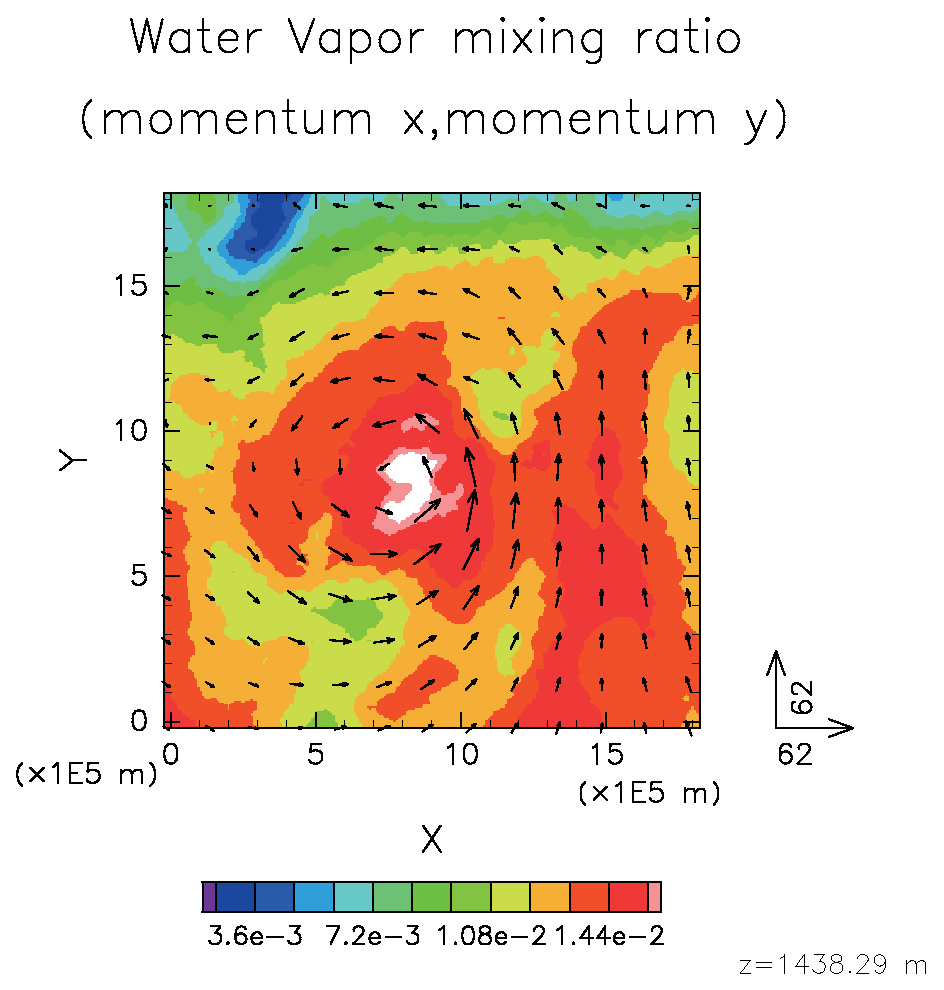
\includegraphics[width=0.7\hsize]{./figure/init_qv-momxy.eps}\\
  \caption{チュートリアル実験の初期場の様子:カラーシェードは高度1.5kmにおける比湿の分布,ベクトルは高度1.5kmにおける水平運動量フラックスを表している.}
  \label{fig:init}
\end{center}
\end{figure}



%-------------------------------------------------------%
\section{時間積分を行う:run}
%-------------------------------------------------------%
\subsubsection{run.confの準備}
ここではいよいよSCALE-LESモデルを実行する.
まず,runディレクトリへ移動する.
\begin{verbatim}
 $ cd ${Tutrial_DIR}/real/run
\end{verbatim}

runディレクトリの中には,\verb|run.conf|という名前の
コンフィグファイルが準備されており、
ドメインの位置や格子点数など、チュートリアル用の設定(Table\ref{tab:grids})に合わせてある.
モデル本体の実行には事前に作成した地形・土地利用データや初期値・境界値データを利用する.
これらのファイルの場所は、\verb|run.conf|内の
\verb|TOPO_IN_BASENAME|,\verb|LANDUSE_IN_BASENAME|,
\verb|RESTART_IN_BASENAME|,および\verb|ATMOS_BOUNDARY_IN_BASENAME|で
指定している.

\begin{verbatim}
  &PARAM_TOPO
   TOPO_IN_BASENAME = "../pp/topo_d01",
  /

  &PARAM_LANDUSE
   LANDUSE_IN_BASENAME  = "../pp/landuse_d01",
  /

  &PARAM_RESTART
   RESTART_OUTPUT      = .false.,
   RESTART_IN_BASENAME = "../init/init_d01_00019094400.000",
  /

  &PARAM_ATMOS_BOUNDARY
   ATMOS_BOUNDARY_TYPE        = "REAL",
   ATMOS_BOUNDARY_IN_BASENAME = "../init/boundary_d01",
   ATMOS_BOUNDARY_USE_VELZ    = .true.,
   ATMOS_BOUNDARY_USE_QHYD    = .false.,
   ATMOS_BOUNDARY_VALUE_VELZ  = 0.0D0,
   ATMOS_BOUNDARY_UPDATE_DT   = 21600.0D0,
  /
\end{verbatim}


\verb|run.conf|の設定の中で時間積分に関する設定は,\verb|PARAM_TIME|の項目にある.
\begin{verbatim}
&PARAM_TIME
 TIME_STARTDATE          = 2014, 8, 10, 0, 0, 0, <- 時間積分を開始する時刻
 TIME_STARTMS            = 0.D0,
 TIME_DURATION           = 12.0D0,  <- 積分期間
 TIME_DURATION_UNIT      = "HOUR",  <- TIME_DURATIONの単位
 TIME_DT                 = 60.0D0,  <- 移流計算の時間ステップ
 TIME_DT_UNIT            = "SEC",   <- TIME_DTの単位
 TIME_DT_ATMOS_DYN       = 15.0D0,  <- 移流計算以外の力学過程の計算の時間ステップ
 TIME_DT_ATMOS_DYN_UNIT  = "SEC",   <- TIME_DT_ATMOS_DYNの単位

 ~~中略~~

/
\end{verbatim}

初期時刻\verb|TIME_STARTDATE|はUTCで指定する.
チュートリアルでは2014年8月10日0時UTCに設定している.
積分のための時間ステップは、上記の他、
それぞれの物理スキーム毎に設定できるようになっている.


計算結果の出力に関する設定は\verb|PARAM_HISTORY|で行う.
\begin{verbatim}
  &PARAM_HISTORY
   HISTORY_DEFAULT_BASENAME  = "history_d01", <-出力するファイル名
   HISTORY_DEFAULT_TINTERVAL = 1800.D0,       <-出力時間間隔
   HISTORY_DEFAULT_TUNIT     = "SEC",         <-出力時間間隔の単位
   HISTORY_DEFAULT_TAVERAGE  = .false.,
   HISTORY_DEFAULT_DATATYPE  = "REAL4",
   HISTORY_DEFAULT_ZINTERP   = .false.,       <- 出力時に高さ面へ内挿するかどうか
   HISTORY_OUTPUT_STEP0      = .true.,        <- 初期時刻(t=0)の値を出力するかどうか
  /
\end{verbatim}
上記の設定に従って、下記の\verb|HISTITEM|に羅列された変数が出力される.
\verb|HISTITEM|ではオプション変数を加えることで、変数毎に、出力間隔を変更したり、
平均値を出力したりすることも可能である.
これらの説明は\ref{sec:output}を参照されたい.

\begin{verbatim}
&HISTITEM item="DENS" /           ! density (3D)
&HISTITEM item="MOMZ" /           ! vertical momentum (3D)
&HISTITEM item="MOMX" /           ! horizontal momentum-x (3D)
&HISTITEM item="MOMY" /           ! horizontal momentum-y (3D)
&HISTITEM item="RHOT" /           ! density * potential-temperature (3D)
&HISTITEM item="QV"   /           ! mixing ratio for vapor (3D)
&HISTITEM item="QHYD" /           ! mixing ratio for hydrometeor (3D)
&HISTITEM item="T"    /           ! temperature (3D)
&HISTITEM item="PRES" /           ! pressure (3D)
&HISTITEM item="U"    /           ! horizontal wind component-x (3D)
&HISTITEM item="V"    /           ! horizontal wind component-y (3D)
&HISTITEM item="W"    /           ! vertical wind component (3D)
&HISTITEM item="PT"   /           ! potential temperature (3D)
&HISTITEM item="RH"   /           ! relative humidity (3D)
&HISTITEM item="PREC" /           ! precipitation (2D)
&HISTITEM item="OLR"  /           ! out-going longwave radiation(2D)
&HISTITEM item="U10" /            ! horizontal wind component-x at 10m height(2D)
&HISTITEM item="V10" /            ! horizontal wind component-y at 10m height(2D)
&HISTITEM item="T2"  /            ! temperature at 2m height (2D)
&HISTITEM item="Q2"  /            ! mixing ratio for vapor at 2m height (2D)
&HISTITEM item="SFC_PRES"   /     ! pressure at the bottom surface (2D)
&HISTITEM item="SFC_TEMP"   /     ! temperature a the bottom surface (2D)
&HISTITEM item="LAND_SFC_TEMP" /  ! temperature a the bottom surface for land model (2D)
&HISTITEM item="URBAN_SFC_TEMP" / ! temperature a the bottom surface for urban model (2D)
\end{verbatim}

その他に実験で使用される物理過程の設定は,
\verb|PARAM_TRACER,PARAM_ATMOS,PARAM_OCEAN,PARAM_LAND,PARAM_URBAN|の項目に
記述されているので,実行前にチェックすること.
詳細なコンフィグファイルの内容については,Appendix \ref{app:namelist}を参照されたい.

%
\subsubsection{実行}
コンパイル済みのバイナリをrunディレクトリへリンクする.

\begin{verbatim}
 $ ln -s ../../bin/scale-les ./
\end{verbatim}
陸面過程や放射過程のモデルを起動するためのパラメータファイルに
リンクを張る.
\begin{verbatim}
 $ ln -s ../../../data/land/* ./   <- 陸面スキーム用のパラメータファイル
 $ ln -s ../../../data/rad/*  ./   <- 放射スキーム用のパラメータファイル
\end{verbatim}
準備が整ったら,4つのMPIプロセスを使用してscale-lesを実行する.
\begin{verbatim}
  $ mpirun -n 4 ./scale-les run.conf < /dev/null >&log&
\end{verbatim}

実行にはおおよそ1時間を要するため,上記のように標準出力をファイルへ
書き出すようにしてバックグラウンドで実行すると便利である.
計算が開始されれば,処理内容のログとして、
\verb|"LOG_d01.pe000000"|ファイルが生成されるので,
例えば下記のようなコマンドで\verb|"LOG_d01.pe000000"|ファイルを参照すれば,
どこまで計算が進んでいるかチェックすることができる.
\begin{verbatim}
 $ tail -f LOG_d01.pe000000
\end{verbatim}
正常にジョブが終了すれば,\verb|history_d01.pe######.nc|と
\verb|restart_d01.pe######.nc|という名前のファイルがMPIプロセス数だけ,
つまり4つずつ生成される(\verb|######|にはMPIプロセスの番号が入る).
historyファイルは計算結果の出力ファイルであり,
\verb|HISTITEM|に指定した変数のみ書き出される.
restartファイルは対応する時刻を開始時刻として
再計算を開始するための初期値ファイルである.
次節でhistoryデータをGrADSで描画可能なバイナリーデータに変換して
結果を確認する方法について説明する.

%####################################################################################


\section{結果を描画する}
\label{sec:quicklook}
%####################################################################################

SCALEモデルの出力ファイルはMPIプロセス毎に出力されるため,
計算領域が分割された状態で出力される.
それぞれのファイルフォーマットは気候・予報(CF)メタデータ規約
に対応したnetcdf4形式である.
ここでは,プロセス毎に分割されたnetcdfファイルをgradsで扱うことがバイナリーファイルにまとめ、いくつか、確認のための図を示す.

\subsubsection{GrADSバイナリーに変換}
%-----------------------------------------------------------------------------------
分割されたnetcdfからGrADSバイナリー変換するには、\verb|netcdf2grads_h|を使用する.
詳細な使用方法は \ref{sec:net2g}節を参照頂きたい.

まず、\ref{sec:source_net2g}節でコンパイルしたバイナリーファイルにリンクを張る.
\begin{verbatim}
 $ ln -s ../../../../util/netcdf2grads_h/net2g ./
\end{verbatim}
ここでは例として、2次元変数であるMSLP、PRECを、
3次元変数として850hPa,500h,200hPa面のU、Vを変換する.
2次元変数のための設定は\verb|net2g.2d.conf|に、
3次元変数のための設定は\verb|net2g.3d.conf|にある.
configureの中のパラメータの設定は\ref{sec:net2g}節を参照頂きたい.

\verb|netcdf2grads_h|で使用可能なプロセス数は、
計算実行時に使用したプロセス数の約数である必要がある.
ここでは、計算に用いたのと同じ4ノード使用して変換することにする.
\begin{verbatim}
 $ mpirun -n 4 ./net2g net2g.2d.conf
 $ mpirun -n 4 ./net2g net2g.3d.conf
\end{verbatim}
成功すれば、下記のファイルが作成される.
\begin{verbatim}
  MSLP_d01z-2d.ctl
  MSLP_d01z-2d.grd
  PREC_d01z-2d.ctl
  PREC_d01z-2d.grd
  U_d01z-3d.ctl
  U_d01z-3d.grd
  V_d01z-3d.ctl
  V_d01z-3d.grd
\end{verbatim}


\subsubsection{計算結果の確認}
%-----------------------------------------------------------------------------------
現在のバージョンの\verb|netcdf2grads_h|では、
SCALEのXY格子座標でのみ、ctlファイルを作成可能である。
今後、緯度経度座標で出力できるようになる予定であるが、
作図の簡便さのために、下記の緯度経度座標で作図するためのctlを別途用意している.
\begin{verbatim}
  MSLP_d01z-2d_lcc.ctl
  PREC_d01z-2d_lcc.ctl
  U_d01z-3d_lcc.ctl
  V_d01z-3d_lcc.ctl
\end{verbatim}

計算結果確認用のサンプル図を作成するための
スクリプト\verb|checkfig.gs|を使って作図する.
\begin{verbatim}
 $ grads -blc checkfig.gs
\end{verbatim}
成功すると、下記の図が作成される.
なお、gradsのバージョンによって文法が異なるので、適宜変更する.
\begin{verbatim}
  mslp.png
  prec.png
  wind.png
\end{verbatim}
下記の図と同じであるか、答え合わせをする.

\begin{figure}[h]
\begin{center}
  \includegraphics[width=0.55\hsize]{./figure/real_mslp.eps}\\
  \caption{計算開始から12時間後の海面更正気圧}
  \label{fig:real_mslp}
\end{center}
\begin{center}
  \includegraphics[width=0.55\hsize]{./figure/real_prec.eps}\\
  \caption{計算開始から12時間後の1時間積算降水量}
  \label{fig:real_prec}
\end{center}
\begin{center}
  \includegraphics[width=0.55\hsize]{./figure/real_wind.eps}\\
  \caption{計算開始から12時間後の500hPaの風速と風ベクトル}
  \label{fig:real_wind}
\end{center}
\end{figure}





\chapter{各種設定: 基礎編}
\label{sec:basic}
\section{対象計算領域の設定}
\label{sec:domain}
%=======================================================================

\subsection{計算領域と解像度、格子点数、MPIプロセスの関係} \label{subsec:relation_dom_reso}
各設定を行う前に、SCALE-RMでの計算領域、解像度、格子点数、MPIプロセスの関係を整理しておく。
計算領域は、水平格子間隔と格子点数を指定することで決定されるようになっている。
図\ref{fig:domain}は、
計算領域、水平格子間隔、格子数、及びMPIプロセス数の関係を示している。
水平方向に2次元の領域分割を行うことで並列化がなされている。

これらは、\namelist{PARAM_INDEX}内の\nmitem{IMAX}、\nmitem{JMAX}、
\namelist{PARAM_PRC}内の\nmitem{PRC_NUM_X}、\nmitem{PRC_NUM_Y}で
水平格子間隔については、\namelist{PARAM_GRD}内の\nmitem{DX}、\nmitem{DY}で
設定する。

ここで、注意すべきことは、「指定する格子点数は各プロセスが受け持つ値」であることである。
設定する格子数(\nmitem{IMAX}, \nmitem{JMAX}, \nmitem{KMAX})は、
1つのMPIプロセスが担当する格子点数を与える仕様となっている。
すなわち、計算領域は、水平格子間隔、格子点数とともに
各方向のMPIプロセス数を考慮して決定する必要がある。

図\ref{fig:domain}に示すように、
MPIプロセス数が$n$(=\verb|PRC_NUM_X|$\times$\verb|PRC_NUM_Y|)の時、
計算領域は、$x$方向に\verb|PRC_NUM_X|個、$y$方向に\verb|PRC_NUM_Y|個に分割される。
以上の関係から、計算領域全体のそれぞれの方向の格子点数および総格子点数は、
\begin{eqnarray}
&& 領域内x方向の格子数 = \left(\verb|IMAX| \times \verb|PRC_NUM_X|\right)
   \times (\verb|KMAX| )  \label{eq:xgridnum}\\
&& 領域内y方向の格子数 = \left(\verb|JMAX| \times \verb|PRC_NUM_Y|
   \times (\verb|KMAX|\right)  \label{eq:ygridnum}\\
&& 領域内の総格子数 = \left(\verb|IMAX| \times \verb|PRC_NUM_X|\right)
   \times (\verb|JMAX| \times \verb|PRC_NUM_Y|)
   \times (\verb|KMAX| )  \nonumber
\end{eqnarray}
の関係となる。
ここで、\verb|KMAX|は、鉛直方向の格子点数であり、
\namelist{PARAM_INDEX}内の項目で指定されている。
次節以降では、MPIプロセス数、格子数、格子間隔、
それぞれの設定方法について詳しく説明する。

\begin{figure}[h]
\begin{center}
  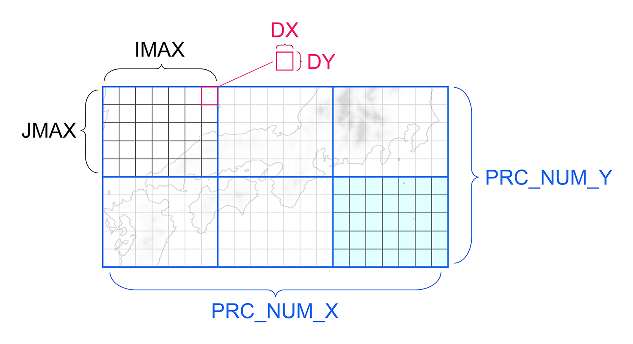
\includegraphics[width=0.8\hsize]{./figure/domain_decomposition.eps}\\
  \caption{計算領域に対する、水平格子間隔(DX, DY)、1MPIプロセスあたりの格子数(IMAX, JMAX)、MPIプロセス数(PRC\_NUM\_X, PRC\_NUM\_Y)の関係。
水色領域は、ある1つのMPIプロセスが担当する領域。}
  \label{fig:domain}
\end{center}
\end{figure}

\subsection{計算領域の設定}

\ref{subsec:relation_dom_reso}節で述べた関係が理解できれば、領域の設定は容易である。
すなわち、式(\ref{eq:xgridnum},\ref{eq:ygridnum})を使って、
\begin{eqnarray}
&& x方向の領域の長さ = x方向の格子点数 \times \verb|DX| \nonumber\\
&& y方向の領域の長さ = y方向の格子点数 \times \verb|DY| \nonumber
\end{eqnarray}
となる。ここで、\nmitem{DX,DY}は、後述するように
\namelist{PRAM_GRID}で指定されるものである。
逆算して、解像度と領域の大きさをを決めて、MPIプロセス数が決まると、
ローカルな領域の格子点数が決まる。

\subsection{MPIプロセス数}

MPIプロセス数は、設定ファイルの\namelist{PARAM_PRC}で指定する。
先に述べた通り、SCALEの入出力ファイルは、MPIプロセス毎に分割されている。
そのため、MPIプロセス数を変更すると分割ファイル数も必ず変わることになる。
従って、例えば、2-MPI並列用に作成した初期値ファイルは、
4-MPI並列のモデル実行には使用できない。
MPIプロセス数を変更するには、
\verb|pp_***.conf|、\verb|init_***.conf|、\verb|run_***.conf| の
すべてを編集・変更し、\verb|pp|, \verb|init| から行う必要がある。\\

\noindent {\small {\gt
\ovalbox{
\begin{tabularx}{140mm}{lX}
\verb|&PARAM_PRC| & \\
\verb| PRC_NUM_X       = 2,| & ; X方向(東西方向)のMPI並列分割数 \\
\verb| PRC_NUM_Y       = 1,| & ; Y方向(南北方向)のMPI並列分割数 \\
\verb|/|\\
\end{tabularx}
}}}\\


全MPIプロセス数は、\verb|PRC_NUM_X| $\times$ \verb|PRC_NUM_Y|  となり、
上記の例では、$x$方向に2分割、$y$方向に1分割(分割なし)の
2-MPI並列ということになる。

実行時にMPIコマンドに指定するMPIプロセス数は、
この総MPIプロセス数を指定しなければならない。
この条件を満たさない場合は、下記のメッセージが
LOGファイルなどに出力されて計算は行われず、直ちに終了する。

\noindent {\small {\gt
\ovalbox{
\begin{tabularx}{140mm}{l}
\verb|xxx total number of node does not match that requested. Check!| \\
\end{tabularx}
}}}\\





\subsection{水平・鉛直格子数}
%-----------------------------------------------------------------------

格子数の設定は、設定ファイル(\verb|***.conf|)の\namelist{PARAM_INDEX}で行う。
\ref{subsec:relation_dom_reso}で詳しく説明したように、以下で設定する水平格子数の値は、
1つのMPIプロセス当たりの値であることに注意が必要である。\\

\noindent {\small {\gt
\ovalbox{
\begin{tabularx}{140mm}{lX}
\verb|&PARAM_INDEX| & \\
\verb| KMAX = 97,|  & 鉛直層数 \\
\verb| IMAX = 20,|  & プロセスあたりのx方向の格子点数 \\
\verb| JMAX = 25,|  & プロセスあたりのy方向の格子点数 \\
\verb|/|\\
\end{tabularx}
}}}\\



\subsection{水平・鉛直格子間隔}
\label{sec:gridinterv}
%-----------------------------------------------------------------------
SCALE-RMでは、水平方向には格子点の位置を均等間隔に設定する。
鉛直方向には均等間隔でも任意の格子点位置を直接指定することもできる。
以下で説明する
\textcolor{red}{\bf 格子間隔の設定は、pp\_***.conf、init\_***.conf、run\_***.confの
設定ファイルの間で一致させなければならないことに注意が必要である。}
\ref{subsec:relation_dom_reso}節で述べたように、
以下で設定する値は、MPIプロセス当たりの値であることに注意が必要である。

%-----------------------------------------------------------------------&
第\ref{sec:buffer}節で述べる緩和領域を覗き、
水平格子間隔は等間隔でしか設定できない。
鉛直格子間隔については、任意に定義することが可能である。
すべての方向について等間隔で設定する場合には、以下のように
設定ファイルの\namelist{PARAM_GRID}の\nmitem{DX,DY,DZ}に
それぞれ、東西、南北、鉛直方向の格子間隔を指定する。
単位はmである。

\noindent {\small {\gt
\ovalbox{
\begin{tabularx}{140mm}{lX}
\verb|&PARAM_GRID  | & \\
\verb| DX = 500.D0,| & ; x方向(東西方向)の格子間隔\\
\verb| DY = 500.D0,| & ; y方向(南北方向)の格子間隔\\
\verb| DZ = 500.D0,| & ; z方向(鉛直方向)の格子間隔\\
\verb|/|\\
\end{tabularx}
}}}\\


以下に、鉛直方向での任意の格子点位置を指定する場合の設定を示す。
鉛直方向は、Lorenz格子を採用しており、
速度成分定義格子点とスカラー定義格子点が半格子分ずれた食い違い格子にになっている。
ここでは、スカラー量を定義している格子点をセンターポイントと呼び、
半格子ズレた格子点をフェイスポイントと呼ぶ(図\ref{fig:scale_grid}参照)。

直接格子点の位置を指定する場合は、フェイスポイントの位置を
\namelist{PARAM_GRID}の中の\nmitem{FZ(:)}で配列として与えればよい。
\footnote{指定の際には、シミュレーションの計算精度
(モデルのコンパイル時に指定した浮動小数点の精度。デフォルトでは倍精度)を用いることが望ましい。}
また、\nmitem{FZ(:)}で指定する値の数は、鉛直層数
(\namelist{PARAM_INDEX}の\nmitem{KMAX})と一致させる必要がある。
例として理想実験のチュートリアルのrun.confファイル
(run\_R20kmDX500m.conf)を下記に示す。

\noindent {\small {\gt
\ovalbox{
\begin{tabularx}{140mm}{lX}
\verb|&PARAM_GRID|     & \\
\verb| DX = 500.D0,|   & x方向の格子間隔(等間隔)[m]\\
\verb| DY = 500.D0,|   & y方向の格子間隔(等間隔)[m]\\
\verb| FZ(:) = |       & z方向のフェイスポイントの位置[m] \\
\verb|    80.000000000000000      ,| & \\
\verb|    168.00000190734863      ,| & \\
\verb|    264.80000610351567      ,| & \\
\verb|     〜 中略 〜|           & \\
\verb|    14910.428862936289      ,| & \\
\verb|    15517.262523292475      ,| & \\
\verb|    16215.121232702089      ,| & \\
\verb|    17017.658748523147      ,| & \\
\verb|    17940.576891717363      ,| & \\
\verb|    19001.932756390710      ,| & \\
\verb|    20222.492000765058      ,| & \\
\verb| BUFFER_DZ = 5000.D0,|          & 第\ref{sec:buffer}節参照\\
\verb| BUFFFACT  =   1.0D0,|          & 第\ref{sec:buffer}節参照\\
\verb|/|\\
\end{tabularx}
}}}\\


\begin{figure}[tb]
\begin{center}
  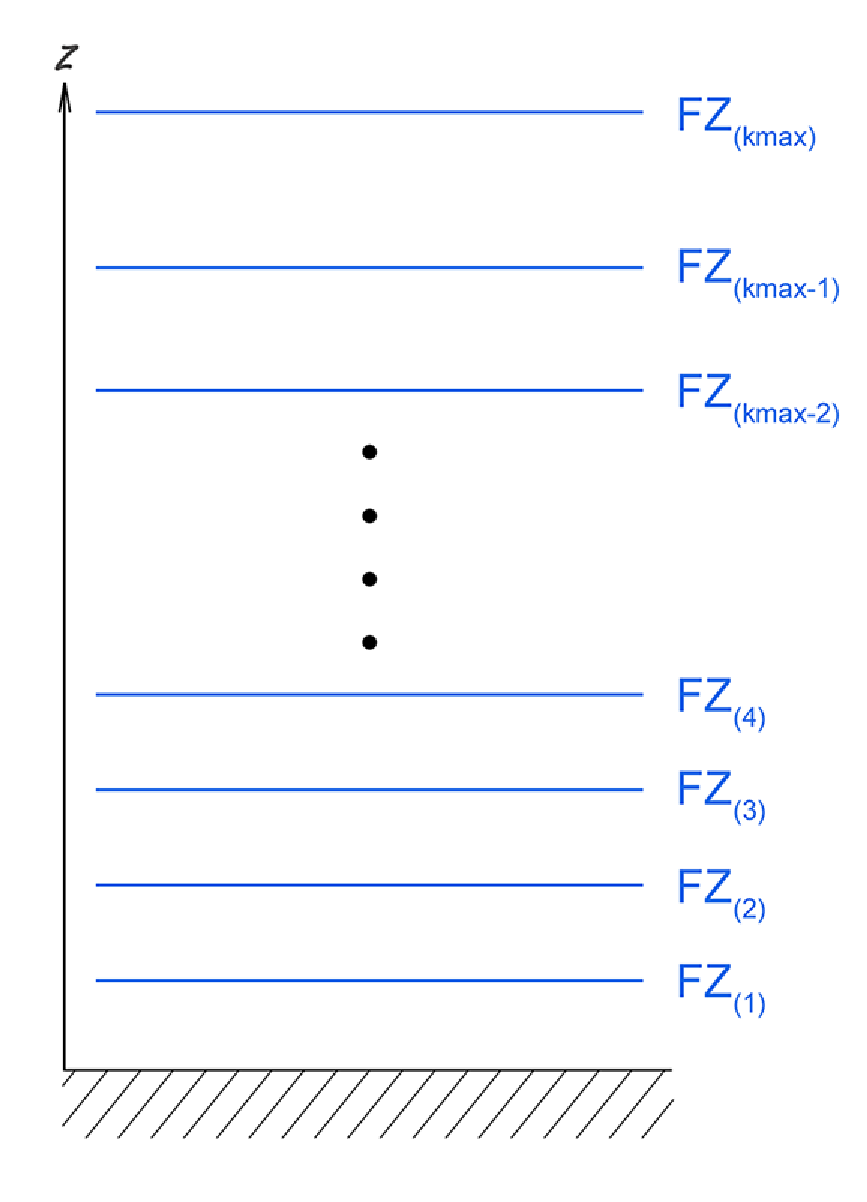
\includegraphics[width=0.4\hsize]{./figure/verticalface.eps}\\
  \caption{SCALE-RMの鉛直格子の定義点。\namelist{PARAM_GRID}で\nmitem{FZ}を指定する時は、ハロを除いた計算領域下端の格子から$k=1$として与える。}
  \label{fig:scale_grid}
\end{center}
\end{figure}
なお、これらの指定では、
標高0mでの格子点として設定され、標高を持つ位置では山岳に沿った座標系によって適切に処理される。


格子点位置は任意に設定できるが、場合によっては計算不安定につながる。
鉛直層の設定については、作成をサポートするツール(\verb|scale/scale-rm/util/makevgrid/|)が
用意されているので参考にされたい。
\footnote{``make\_vgrid.f90''というFortranプログラムと
いくつかのサンプルnamelistが用意されている。}
ツールをコンパイルして実行すれば直ちに設定ファイルに貼り付けて使用できる
\nmitem{FZ(:)}の値が作成される。

\section{力学スキームの設定}
\label{sec:basic_dyn}
%------------------------------------------------------


\subsection{数値解法}
%------------------------------------------------------
設定は、confファイルの\verb|PARAM_ATMOS|の\verb|ATMOS_DYN_TYPE|で設定する。\\

\noindent {\gt\small
\ovalbox{
\begin{tabularx}{140mm}{ll}
\verb|&PARAM_ATMOS  | & \\
\verb| ATMOS_DYN_TYPE    = "HEVI", | & ; \verb|HEVI|: 水平陽解法-鉛直陰解法\\
                                     & ; \verb|HEVE|: 陽解法\\
\verb|/             | & \\
\end{tabularx}
}}\\


\subsection{時間・空間差分スキーム}
%------------------------------------------------------
設定は、confファイルの\verb|PARAM_ATMOS_DYN|で設定する。
また、空間スキームによってはHaloの設定も必要である。
スキームと各種設定については表\ref{tab:nml_atm_dyn}を参照のこと。\\

\noindent {\gt\small
\ovalbox{
\begin{tabularx}{140mm}{ll}
 \verb|&PARAM_ATMOS_DYN  | & \\
 \verb|ATMOS_DYN_TINTEG_SHORT_TYPE          = RK4,|       & ; 時間スキームより選択\\
 \verb|ATMOS_DYN_TINTEG_TRACER_TYPE         = RK3WS2002,| & ; 時間スキームより選択\\
 \verb|ATMOS_DYN_FVM_FLUX_TYPE              = CD4,|       & ; 空間スキームより選択\\
 \verb|ATMOS_DYN_FVM_FLUX_TRACER_TYPE       = UD3KOREN1993,| & ; 空間スキームより選択\\
 \verb|ATMOS_DYN_FLAG_FCT_TRACER            = .false.,|   & ; FCTスキームを利用するかどうか\\
 \verb|ATMOS_DYN_NUMERICAL_DIFF_COEF        = 1.D-2, |    & \\
 \verb|ATMOS_DYN_NUMERICAL_DIFF_COEF_TRACER = 0.D0, |     & \\
 \verb|ATMOS_DYN_enable_coriolis            = .true.,|    & \\
\verb|/             | & \\
\end{tabularx}
}}\\



\begin{table}[h]
\begin{center}
  \caption{力学スキームの設定}
  \label{tab:nml_atm_dyn}
  \begin{tabularx}{150mm}{llXX} \hline
    \rowcolor[gray]{0.9} & \multicolumn{1}{l}{設定名} & \multicolumn{1}{l}{スキーム名} & \\ \hline
    \multicolumn{3}{l}{時間スキーム} & 推奨の\verb|TIME_DT_ATMOS_DYN|と\verb|TIME_DT| \\ \hline
    & \multicolumn{1}{l}{\verb|RK3|} & \multicolumn{1}{l}{Heun's 3rd order Runge-Kutta scheme} & \multicolumn{1}{l}{XX sec, XX sec}\\
    & \multicolumn{1}{l}{\verb|RK3WS2002|} & \multicolumn{1}{X}{Wicker and Skamarock (2002) 3段ルンゲクッタスキーム} & \multicolumn{1}{l}{XX sec, XX sec}\\
    & \multicolumn{1}{l}{\verb|RK4|} & \multicolumn{1}{l}{4th order Runge-Kutta scheme} & \multicolumn{1}{l}{XX sec, XX sec}\\
    \hline
    \multicolumn{3}{l}{空間スキーム} & 最小の設定格子数(Haloの数)\\ \hline
    & \multicolumn{1}{l}{\verb|CD2|} & \multicolumn{1}{l}{2-nd order central difference schemes} & \multicolumn{1}{l}{1}\\
    & \multicolumn{1}{l}{\verb|CD4|} & \multicolumn{1}{l}{4-th order central difference schemes} & \multicolumn{1}{l}{2}\\
    & \multicolumn{1}{l}{\verb|CD6|} & \multicolumn{1}{l}{6-th order central difference schemes} & \multicolumn{1}{l}{3}\\
    & \multicolumn{1}{l}{\verb|UD3|} & \multicolumn{1}{l}{3-rd order upwind difference schemes} & \multicolumn{1}{l}{2}\\
    & \multicolumn{1}{l}{\verb|UD5|} & \multicolumn{1}{l}{5-th order upwind difference schemes} & \multicolumn{1}{l}{3}\\
    & \multicolumn{1}{l}{\verb|UD3KOREN1993|} & \multicolumn{1}{X}{3-rd order upwind difference schemes with Koren (1993) filter} & \\
\hline
  \end{tabularx}
\end{center}
\end{table}

トレーサー移流については、何らかの非負保証スキームを使う事が望ましい。つまり \verb|ATMOS_DYN_FLUX_TRACER_TYPE| として \verb|UD3KOREN1993| 以外を選択した場合は、\verb|ATMOS_DYN_FLAG_FCT_TRACER| を \verb|.true.| としてFCTを利用するのがよい。


空間スキームがCD4, UD3以外の場合(Haloの数が2以外の場合)、Haloの設定も必要である。
Haloの数は、n次の空間スキームに対して$\lceil n/2 \rceil$である。ここで、$\lceil \rceil$ は天井感数である。\\

\noindent {\gt\small
\ovalbox{
\begin{tabularx}{140mm}{ll}
 \verb|&PARAM_INDEX | &  \\
 \verb| IHALO = 2,|   & ; $\lceil n/2 \rceil$を設定\\
 \verb| JHALO = 2,|   & ; $\lceil n/2 \rceil$を設定\\
 \verb|/ | & \\
\end{tabularx}
}}\\

\section{物理スキームの設定} \label{sec:basic_physics}
%------------------------------------------------------

\subsection{雲微物理スキーム} \label{sec:basic_microphys}
%------------------------------------------------------
雲微物理スキームの選択は、init.confとrun.conf中の
\verb|PARAM_TRACER|の\verb|TRACER_TYPE|、
及び、\verb|PARAM_ATMOS|の\verb|ATMOS_PHY_MP_TYPE|で設定する。
このとき{\color{red}{\verb|TRACER_TYPE|と\verb|ATMOS_PHY_MP_TYPE|は同じものを設定し}}
、かつ、\textcolor{red}{init.conf,run.confで同一の設定}とする必要がある。
雲微物理スキームを計算する(callする)タイミングは、
\verb|PARAM_TIME|で設定するが、これについては
第\ref{sec:timeintiv}節を参照のこと。\\



\noindent {\gt
\ovalbox{
\begin{tabularx}{140mm}{ll}
\verb|&PARAM_ATMOS  | & \\
\verb| ATMOS_PHY_MP_TYPE = "TOMITA08", | & ; 表\ref{tab:nml_atm_mp}より選択。\\
\verb|/             | & \\
\\
\verb|&PARAM_TRACER | & \\
\verb| TRACER_TYPE = ``TOMITA08'', | & \verb|ATMOS_PHY_MP_TYPE|と同じスキーム。\\
\verb|/             | & \\
\end{tabularx}
}}\\

\begin{table}[h]
\begin{center}
  \caption{雲微物理スキームの設定}
  \label{tab:nml_atm_mp}
  \begin{tabularx}{150mm}{lXX} \hline
    \rowcolor[gray]{0.9}  設定名 & スキームの説明 & 文献\\ \hline
     \verb|OFF|      & \textcolor{雲微物理を使用しないが、$TRACER_TYPE$で指定した雲微物理に対応した予報変数を含める} &  \\
     \verb|DRY|      & \textcolor{雲物理を使用しない(予報変数に雲微物理に関連した変数を一切含めない)} &  \\
     \verb|KESSLER|  & 水雲のみの1-momentバルク法 & \citet{kessler_1969} \\
     \verb|TOMITA08| & 氷雲を含む1-momentバルク法 & \citet{tomita_2008} \\
     \verb|SN14|     & 氷雲を含む2-momentバルク法 & \citet{sn_2014} \\
     \verb|SUZUKI10| & 1-momentビン法(氷雲を含むか否かはオプションで選択) & \citet{suzuki_etal_2010} \\
    \hline
  \end{tabularx}
\end{center}
\end{table}

\verb|SUZUKI10|以外を選択した場合は、
init.conf、run.confのTRACER\_TYPEとATMOS\_PHY\_MP\_TYPEを
変更するだけで実行可能である。


\subsubsection{SUZUKI10}
%---------------------------
\verb|ATMOS_PHY_MP_TYPE = "SUZUKI10"|を選択した場合は、init.conf、run.confの双方に
下記を追加する必要がある。\\

\noindent {\gt
\ovalbox{
\begin{tabularx}{140mm}{ll}
\verb|&PARAM_BIN|   &  \\
\verb| nbin   = 33, & (ビンの数)| \\
\verb| ICEFLG =  1, & (氷雲を考慮するか否か,0->水雲のみ,1->氷雲も含む)| \\
\verb|/|            & \\
\end{tabularx}
}}\\

この場合も、
{\color{red}{init.confとrun.confに記載される\verb|PARAM_BIN|は同一にする必要がある}}。
\verb|SUZUKI10|を選択した時には、micpara.datという
雲微物理の計算に必要なファイルが自動生成される。
micpara.datがすでに存在する場合はあるものを利用するが、
nbinが変わると新たに作成しなければならない。
micpara.datの1行目にnbinの情報が記載されているが、
もしrun.confに記載されるnbinと
micpara.datに記載されているnbinが異なれば、\\

\noindent {\gt
\fbox{
\begin{tabularx}{140mm}{l}
\verb|xxx nbin in inc_tracer and nbin in micpara.dat is different check!| \\
\end{tabularx}
}}\\

\noindent というエラーメッセージを標準出力に出力して計算が落ちるようになっている。
そのため、nbinを変更した際は、micpara.datを消去して
新たに作り直す必要がある
(micpara.datを消して再度SCALEをSUZUKI10を用いて実行すれば自動的に新しいmicpara.datが生成される)。



\subsection{乱流スキーム} \label{sec:basic_turbulence}
%------------------------------------------------------

乱流スキームの選択は,init.confとrun.conf中の
\verb|PARAM_ATMOS|の\verb|ATMOS_PHY_TB_TYPE|で設定する。
乱流スキームを計算する(callする)タイミングは、
\verb|PARAM_TIME|で設定するが、これについては
第\ref{sec:timeintiv}節を参照のこと。\\

\noindent {\gt
\ovalbox{
\begin{tabularx}{140mm}{ll}
\verb|&PARAM_ATMOS  | & \\
\verb| ATMOS_PHY_TB_TYPE = "MYNN", | & ; 表\ref{tab:nml_atm_tb}より選択。\\
\verb|/             | & \\
\end{tabularx}
}}\\

\begin{table}[h]
\begin{center}
  \caption{乱流スキームの設定}
  \label{tab:nml_atm_tb}
  \begin{tabularx}{150mm}{lXX} \hline
    \rowcolor[gray]{0.9}  設定名 & スキームの説明 & 文献\\ \hline
      \verb|OFF|          & \textcolor{red}{使用しない,どういう状態を想定?} &  \\
      \verb|SMAGORINSKY|  & Smagorinsky typeのサブグリッドモデル    & \citet{smagorinsky_1963,lilly_1962,Brown_etal_1994,Scotti_1993} \\
      \verb|D1980|        & Deardorff(1980)サブグリットモデル &\citet{Deardorff_1980} \\
      \verb|MYNN|         & MYNN Level 2.5 乱流モデル & \citet{my_1982,nakanishi_2004} \\
      \verb|HYBRID|       & MYNN と SMAGORINSKYのハイブリット &  \\
    \hline
  \end{tabularx}
\end{center}
\end{table}




\subsection{放射スキーム} \label{sec:basic_radiation}
%------------------------------------------------------
放射スキームの選択は、init.confとrun.conf中の
\verb|PARAM_ATMOS|の\verb|ATMOS_PHY_RD_TYPE|で設定する。
放射スキームを計算する(callする)タイミングは、
\verb|PARAM_TIME|で設定するが、これについては
第\ref{sec:timeintiv}節を参照のこと。\\

\noindent {\gt
\ovalbox{
\begin{tabularx}{140mm}{ll}
\verb|&PARAM_ATMOS  | & \\
\verb| ATMOS_PHY_RD_TYPE = "MSTRN", | & ; 表\ref{tab:nml_atm_rd}より選択。\\
\verb|/             | & \\
\end{tabularx}
}}\\

\begin{table}[h]
\begin{center}
  \caption{放射スキームの選択肢}
  \label{tab:nml_atm_rd}
  \begin{tabularx}{150mm}{lXX} \hline
    \rowcolor[gray]{0.9}  設定名 & スキームの説明 & 文献\\ \hline
      \verb|OFF|    & \textcolor{red}{使用しない, どういう状態を想定?} &  \\
      \verb|MSTRN|  & MSTRN-X    & \citet{sekiguchi_2008} \\
    \hline
  \end{tabularx}
\end{center}
\end{table}

\verb|MSTRN|を実行するには、各種外部データとパラメタテーブルが必要である。
オゾンのプロファイルなどの外部データとパラメタテーブルは、
\begin{verbatim}
  scale-rm/test/data/rad/
\end{verbatim}
に用意されている。
放射スキームを利用する場合は、これらのファイルが必要となる。



\subsection{地表面(大気下端境界)} \label{sec:basic_surface}
%------------------------------------------------------
大気下端境界の設定は、init.confとrun.conf中の
\verb|PARAM_ATMOS|の\verb|ATMOS_PHY_SF_TYPE|で設定する。\\

\noindent {\gt
\ovalbox{
\begin{tabularx}{140mm}{ll}
\verb|&PARAM_ATMOS  | & \\
\verb| ATMOS_PHY_SF_TYPE = "COUPLE", | & ; 表\ref{tab:nml_atm_sf}より選択。\\
\verb|/             | & \\
\end{tabularx}
}}\\

\begin{table}[h]
\begin{center}
  \caption{大気下端境界の選択肢}
  \label{tab:nml_atm_sf}
  \begin{tabularx}{150mm}{lX} \hline
    \rowcolor[gray]{0.9}  設定名 & スキームの説明              \\ \hline
      \verb|OFF|     & \textcolor{red}{ゼロフラックスを想定}   \\
      \verb|CONST|   & Surface fluxを任意の値に固定             \\ %詳細は、表\ref{tab:sfcflux}参照。
      \verb|BULK|    & バルクモデル \textcolor{red}{これって陸面バルクとどう違うの? パラメータだけ?海想定?}  \\
      \verb|COUPLE|  & 海・陸面・都市モデル使用する場合に選択   \\
    \hline
  \end{tabularx}
\end{center}
\end{table}

地表面スキームをcallするタイミングは、
\verb|PARAM_TIME|で設定するが、これについては
第\ref{sec:timeintiv}節を参照のこと。


\subsubsection{CONST設定}
%---------------------------
\verb|ATMOS_PHY_SF_TYPE = "CONST"|を選択した場合は、run.confで
下記を設定することにより、任意の値に固定することが可能である。
下記の値はデフォルトの設定を示す。\\

\noindent {\small {\gt
\ovalbox{
\begin{tabularx}{150mm}{lX}
 \\
 \verb|&PARAM_ATMOS_PHY_SF_CONST                | & \\
 \verb| ATMOS_PHY_SF_FLG_MOM_FLUX   =    0      | & 0: Bulk coefficient is constant \\
                                                  & 1: Friction velocity is constant \\
 \verb| ATMOS_PHY_SF_U_minM         =    0.0_DP | & Minimum limit of absolute velocity for momentum [m/s] \\
 \verb| ATMOS_PHY_SF_Const_Cm       = 0.0011_DP | & Constant bulk coefficient for momentum [NIL] \\
                                                  &  (\verb|ATMOS_PHY_SF_FLG_MOM_FLUX = 0| のとき有効) \\
 \verb| ATMOS_PHY_SF_CM_min         = 1.0E-5_DP | & Minimum limit of bulk coefficient for momentum [NIL] \\
                                                  &  (\verb|ATMOS_PHY_SF_FLG_MOM_FLUX = 1| のとき有効) \\
 \verb| ATMOS_PHY_SF_Const_Ustar    =   0.25_DP | & Constant friction velocity [m/s] \\
                                                  &  (\verb|ATMOS_PHY_SF_FLG_MOM_FLUX = 1| のとき有効) \\
 \verb| ATMOS_PHY_SF_Const_SH       =   15.0_DP | & Constant surface sensible heat flux [W/m2] \\
 \verb| ATMOS_PHY_SF_FLG_SH_DIURNAL =  .false.  | & Diurnal modulation for sensible heat flux? [logical]\\
 \verb| ATMOS_PHY_SF_Const_FREQ     =   24.0_DP | & Frequency of sensible heat flux modulation [hour]\\
 \verb| ATMOS_PHY_SF_Const_LH       =  115.0_DP | & Constant surface latent   heat flux [W/m2] \\
 \verb|/|            & \\
 \\
\end{tabularx}
}}}\\


\subsection{海洋スキーム(大気-海面フラックス)} \label{sec:basic_ocean}
%------------------------------------------------------

海洋スキームをONにする場合、
\verb|&PARAM_ATMOS|の\verb|ATMOS_PHY_SF_TYPE = "COUPLE"|とする必要がある。
海洋スキームの選択は、init.confとrun.conf中の
\verb|PARAM_OCEAN|の\verb|OCEAN_TYPE|で設定する。
海洋スキームを計算(フラックスをupdate)するタイミングは、
\verb|PARAM_TIME|で設定するが、これについては
第\ref{sec:timeintiv}節を参照のこと。\\

\noindent {\gt
\ovalbox{
\begin{tabularx}{140mm}{ll}
\verb|&PARAM_ATMOS  | & \\
\verb| ATMOS_PHY_SF_TYPE = "COUPLE", | &\\
\verb|/             | & \\
\\
\verb|&PARAM_OCEAN  | & \\
\verb| OCEAN_TYPE = "CONST", | & ; 表\ref{tab:nml_ocean}より選択。\\
\verb|/             | & \\
\end{tabularx}
}}\\

\begin{table}[h]
\begin{center}
  \caption{海洋スキームの選択肢}
  \label{tab:nml_ocean}
  \begin{tabularx}{150mm}{lX} \hline
    \rowcolor[gray]{0.9}  設定名 & スキームの説明 \\ \hline
      \verb|OFF|   & 土地利用にOCEANがない場合のみ使用可    \\
      \verb|CONST| & 初期値固定                              \\
      \verb|FILE|  & 外部ファイルから与える (時間変化あり)   \\
      \verb|SLAB|  & 海洋スラブモデル                        \\
    \hline
  \end{tabularx}
\end{center}
\end{table}


\subsubsection{海洋スラブモデル}
%---------------------------
\verb|OCEAN_TYPE = "SLAB"|を選択した場合は、init.confとrun.confで
モデルの深さを設定することができる。\\

\noindent {\gt
\ovalbox{
\begin{tabularx}{140mm}{ll}
 \verb|&PARAM_OCEAN_PHY_SLAB                 | & \\
 \verb|  OCEAN_PHY_SLAB_DEPTH   = 10.0_DP,   | & ; デフォルト設定 \\
 \verb|/|            & \\
\end{tabularx}
}}\\


\subsubsection{外部ファイル入力}
%---------------------------
\verb|OCEAN_TYPE = "FILE"|を選択した場合は、init.confとrun.confで
外部入力ファイルの設定が必要である。\\

\noindent {\gt
\ovalbox{
\begin{tabularx}{140mm}{ll}
 \verb|&EXTITEM            |                       & \\
 \verb| basename   = "../init/output/ocean_d01", | & ; 入力ファイル\\
 \verb| varname    = "OCEAN_TEMP",               | & ; \verb|"OCEAN_TEMP"|と書く。\\
 \verb| step_limit = 1800, |                        & \\
 \verb| step_fixed =  -1,  |                        & \\
 \verb| enable_periodic_year  = .false.,|           & \\
 \verb| enable_periodic_month = .false.,|           & \\
 \verb| enable_periodic_day   = .false.,|           & \\
 \verb|/|            & \\
\end{tabularx}
}}\\



\subsection{陸面モデル(大気-陸面フラックス)} \label{sec:basic_land}
%------------------------------------------------------
陸面モデルをONにする場合、
\verb|&PARAM_ATMOS|の\verb|ATMOS_PHY_SF_TYPE = "COUPLE"|である必要がある。
陸面モデルの選択は、init.confとrun.conf中の
\verb|PARAM_LAND|の\verb|LAND_TYPE|で設定する。
陸面モデルを計算する(callする)タイミングは、
\verb|PARAM_TIME|で設定するが、これについては
第\ref{sec:timeintiv}節を参照のこと。\\

\noindent {\gt
\ovalbox{
\begin{tabularx}{140mm}{ll}
\verb|&PARAM_ATMOS  | & \\
\verb| ATMOS_PHY_SF_TYPE = "COUPLE", | & \\
\verb|/             | & \\
\\
\verb|&PARAM_LAND  | & \\
\verb| LAND_TYPE = "SLAB", | & ; 表\ref{tab:nml_land}より選択。\\
\verb|/             | & \\
\end{tabularx}
}}\\

\begin{table}[h]
\begin{center}
  \caption{陸面スキームの選択肢}
  \label{tab:nml_land}
  \begin{tabularx}{150mm}{llX} \hline
    \rowcolor[gray]{0.9}  設定名 & スキームの説明 & 文献\\ \hline
      \verb|CONST| & 土壌温度・土壌水分・地表面温度 初期値固定 &  \\
      \verb|SLAB|  & 熱拡散、バケツモデルモデル   &  \\
    \hline
  \end{tabularx}
\end{center}
\end{table}



\subsubsection{陸面スラブモデル}
%---------------------------
\verb|LAND_TYPE = "SLAB"|を選択した場合は、
土地利用データとそれに対応するパラメタテーブルが必要である。
パラメタテーブルは、
\begin{verbatim}
  scale-rm/test/data/land/param.bucket.conf
\end{verbatim}
に用意されている。
ファイルには、各土地利用区分とそれに対応する粗度長などのパラメタが与えられている。
陸面スラブモデルを使用する場合は、このパラメタテーブルが必要である。


フラックス計算に使用するバルク交換係数の計算スキームは 
run.conf中の\verb|PARAM_BULKFLUX|の\verb|BULKFLUX_TYPE|で設定する。\\

\noindent {\gt
\ovalbox{
\begin{tabularx}{140mm}{ll}
\verb|&PARAM_BULKFLUX  | & \\
\verb| BULKFLUX_TYPE = "B91W01", | & ; 表\ref{tab:nml_bulk}より選択。\\
\verb|/             | & \\
\end{tabularx}
}}\\

\begin{table}[h]
\begin{center}
  \caption{バルクフラックススキームの選択肢}
  \label{tab:nml_bulk}
  \begin{tabularx}{150mm}{llX} \hline
    \rowcolor[gray]{0.9}  設定名 & スキームの説明 & 文献\\ \hline
      \verb|B91W01| & デフォルト & \citet{beljaars_1991,wilson_2001}\\
      \verb|U95|    &            & \citet{uno_1995}\\
    \hline
  \end{tabularx}
\end{center}
\end{table}




\subsection{都市モデル(大気-都市面フラックス)} \label{sec:basic_urban}
%------------------------------------------------------

都市モデルをONにする場合、
\verb|&PARAM_ATMOS|の\verb|ATMOS_PHY_SF_TYPE = "COUPLE"|である必要がある。
都市モデルの選択は、init.confとrun.conf中の
\verb|PARAM_URBAN|の\verb|URBAN_TYPE|で設定する。
都市モデルを計算する(callする)タイミングは、
\verb|PARAM_TIME|で設定するが、これについては
第\ref{sec:timeintiv}節を参照のこと。\\

\noindent {\gt
\ovalbox{
\begin{tabularx}{140mm}{ll}
\verb|&PARAM_ATMOS  | & \\
\verb| ATMOS_PHY_SF_TYPE = "COUPLE", | &\\
\verb|/             | & \\
\\
\verb|&PARAM_URBAN  | & \\
\verb| URBAN_TYPE="SLC", | & ; 表\ref{tab:nml_urban}より選択。\\
\verb|/             | & \\
\end{tabularx}
}}\\

\begin{table}[h]
\begin{center}
  \caption{都市スキームの選択肢}
  \label{tab:nml_urban}
  \begin{tabularx}{150mm}{llX} \hline
    \rowcolor[gray]{0.9}  設定名 & スキームの説明 & 文献\\ \hline
      \verb|SLC|  & 単層キャノピーモデル   & \citet{kusaka_2001} \\
    \hline
  \end{tabularx}
\end{center}
\end{table}





\chapter{各種設定: 実用編}
\label{sec:advance}
\section{単精度実行} \label{sec:single}
%------------------------------------------------------








\section{地図投影法と計算領域の位置} \label{sec:adv_mapproj}
%------------------------------------------------------
計算領域の位置と投影法は、configファイルの\verb|PARAM_MAPPROJ|の項目を編集することで設定できる。
\textcolor{red}{\bf この設定も、pp\_***.conf、init\_***.conf、run\_***.confのconfigファイルの間で
必ず一致させなければならない。}はじめに下記の例をもとに説明する。\\

\noindent {\small {\gt
\ovalbox{
\begin{tabularx}{140mm}{l}
\verb|&PARAM_MAPPROJ| \\
\verb| MPRJ_basepoint_lon = 138.727778D0,| \\
\verb| MPRJ_basepoint_lat = 35.360556D0,| \\
\verb| MPRJ_type          = 'MER',| \\
\verb|/| \\
\end{tabularx}
}}}\\

\noindent まず\verb|MPRJ_basepoint_lat|と\verb|MPRJ_basepoint_lon|は、計算領域の中心の緯度・経度を表す。
SCALEでは、北緯を正、南緯を負の値として表現し、経度は0度を起点に右回りで表現するため、この設定では計算領域の
中心が北緯35.360556度、東経138.727778度に位置することになる。この場所を中心に指定された大きさで、計算領域が
設定される\footnote{デフォルトではメルカトル図法に基づいて緯度・経度を計算する際の基準とする緯度は、
MPRJ\_basepoint\_latの値が使用されるが、MPRJ\_M\_latを用いて任意の緯度を指定することもできる。}。
実際にはSCALE内部での格子点は実距離に基づいて格子点が配置されるので、投影法で設定されるのは、
実距離に基づいた緯度・経度座標が計算される。この緯度・経度情報は、すべてのSCALEのNetCDF形式の出力ファイルに
含まれている。

\verb|MPRJ_type|は、地図投影法の種類を表しており、\verb|MER|はメルカトル図法を意味する。
SCALEで現在選択できる地図投影法とその指定文字列は次のとおりである。

\begin{table}[htb]
\begin{center}
\caption{SCALEで選択できる地図投影法}
\begin{tabularx}{150mm}{|l|X|} \hline
 \rowcolor[gray]{0.9} 地図投影法 & \verb|MPRJ_type| \\ \hline
 地図投影なし(理想実験用)& \verb|NONE| \\ \hline
 ランベルト正角円錐図法 & \verb|LC| \\ \hline
 極心平射図法(ポーラーステレオ) & \verb|PS| \\ \hline
 メルカトル図法 & \verb|MER| \\ \hline
 正距円筒図法 & \verb|EC| \\ \hline
\end{tabularx}
\label{tab:map_proj}
\end{center}
\end{table}

メルカトル図法以外の投影法も、\verb|MPRJ_type|の指定を変更するだけで、上記と同じように使用可能であるが、
ランベルト正角円錐図法の設定方法については、設定方法が異なるため以下で説明する。ここでは、現実大気実験
チュートリアルで使用した\verb|run.conf|ファイルを例に挙げる。\\

\noindent {\small {\gt
\ovalbox{
\begin{tabularx}{140mm}{l}
\verb|&PARAM_MAPPROJ| \\
\verb| MPRJ_basepoint_lon = 135.220404D0,| \\
\verb| MPRJ_basepoint_lat = 34.653396D0,| \\
\verb| MPRJ_type          = 'LC',| \\
\verb| MPRJ_LC_lat1       =  30.00D0,| \\
\verb| MPRJ_LC_lat2       =  40.00D0,| \\
\verb|/| \\
\end{tabularx}
}}}\\

SCALEでは``standard parallel type''の実装を採用しているため、投影を決定する上で2つの``standard latitude''の
位置を指定する必要がある。2つのstandard latitudeに挟まれた領域では、緯線・経線の長さの比が地球楕円体面上における
長さの比と近くなるように調節される。従って、メルカトル図法の場合に比べて、standard latitudeを設定する
\verb|MPRJ_LC_lat1|と\verb|MPRJ_LC_lat2|の項目が追加されている。それぞれ、南側、北側のstandard latitudeの
値を``degree''で指定する。

さらに下記のように\verb|MPRJ_basepoint_x|と\verb|MPRJ_basepoint_y|という変数を用いることで、地図投影中心と
計算領域中心をずらすこともできる。\\

\noindent {\small {\gt
\ovalbox{
\begin{tabularx}{140mm}{l}
\verb|&PARAM_MAPPROJ| \\
\verb| MPRJ_basepoint_lon = 135.220404D0,| \\
\verb| MPRJ_basepoint_lat = 34.653396D0,| \\
\verb| MPRJ_basepoint_x   = 100.0D0,| \\
\verb| MPRJ_basepoint_y   = 100.0D0,| \\
\verb| MPRJ_type          = 'LC',| \\
\verb| MPRJ_LC_lat1       =  30.00D0,| \\
\verb| MPRJ_LC_lat2       =  40.00D0,| \\
\verb|/| \\
\end{tabularx}
}}}\\

\noindent \verb|MPRJ_basepoint_x|と\verb|MPRJ_basepoint_y|は、地図投影中心の位置を、計算領域の南西端(左下角)から
の距離で指定するパラメータで、単位はメートルである。これらを指定しない場合は、デフォルト設定として計算領域中心と
地図投影中心の位置は一致する。上記の場合とデフォルト設定の場合を比較したものが図\ref{fig:map_lc}である。
図\ref{fig:map_lc}aはデフォルト設定で投影中心と計算領域中心が一致している場合、図\ref{fig:map_lc}bは、
計算領域の位置を投影中心からずらした場合の関係を表している。図\ref{fig:map_lc}bでは、計算領域の南西端から
\verb|MPRJ_basepoint_x|と\verb|MPRJ_basepoint_y|で指定した距離だけ離れた位置に投影中心がある。

\begin{figure}[t]
\begin{center}
  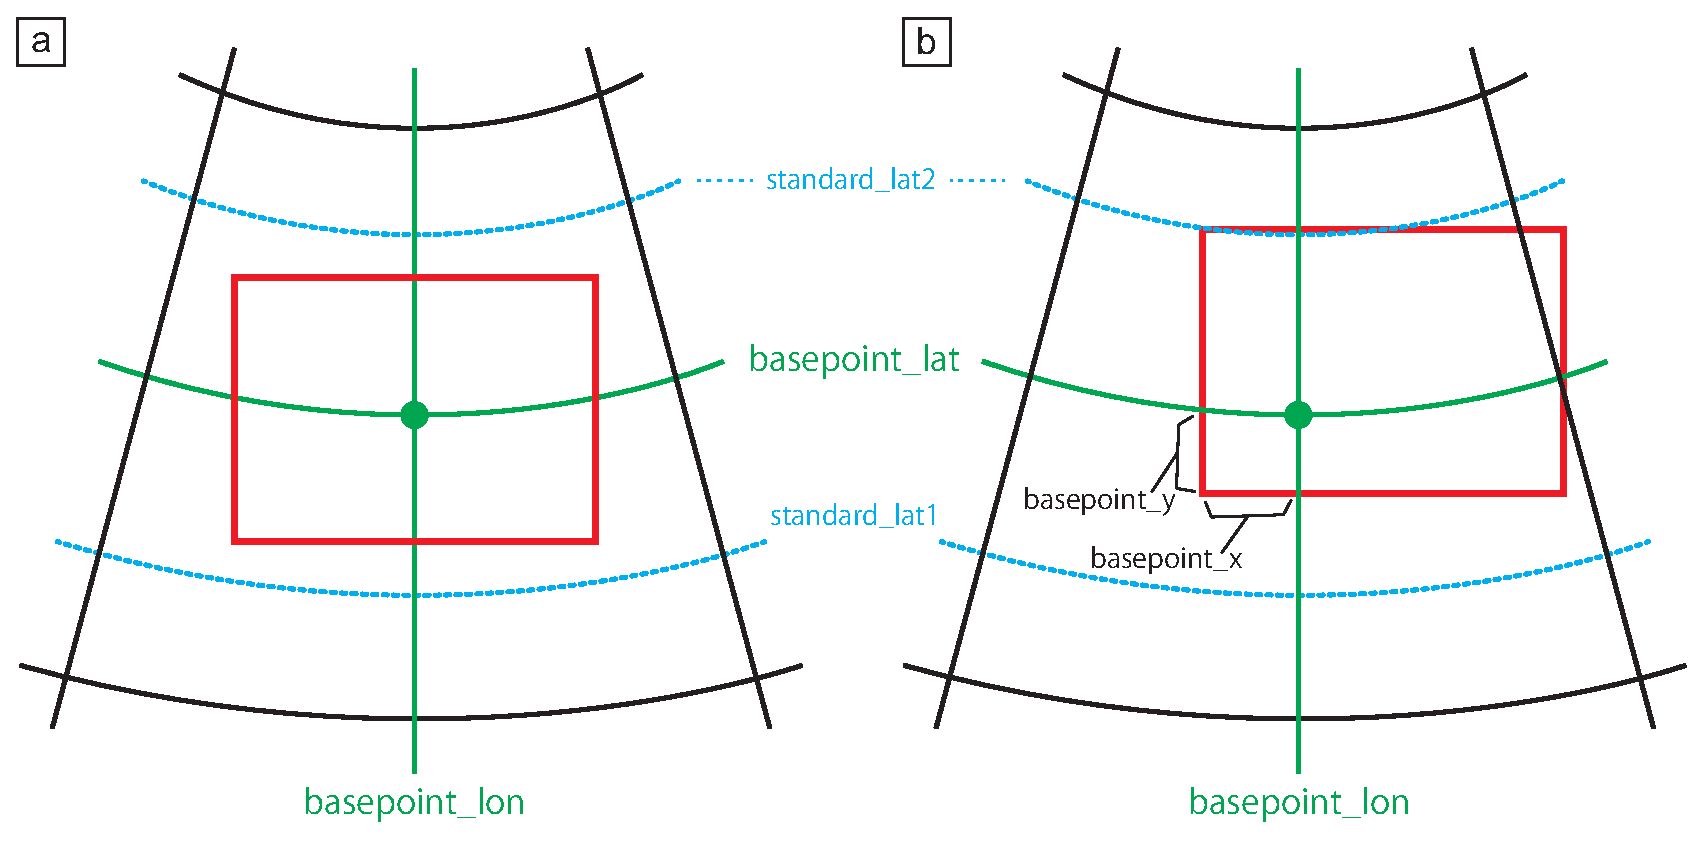
\includegraphics[width=0.8\hsize]{./figure/LC_latlon_xy.eps}\\
  \caption{投影中心と計算領域の関係:(a)はデフォルト設定の場合、(b)は計算領域の位置を投影中心からずらした場合。
  赤線の矩形が計算領域を表す。}
  \label{fig:map_lc}
\end{center}
\end{figure}


\subsection{側面境界条件} \label{sec:adv_lateralbnd}
%------------------------------------------------------
SCALEでは、側面境界条件として「周期境界条件」と「外部入力データ指定」の2種類から選択できる。デフォルトの設定は東西方向、
南北方向ともに周期境界条件となっている。主に理想実験では周期境界条件を使用し、現実大気実験では外部入力データ指定
を使用することを想定している。設定方法によっては、他の側面境界条件も設定可能であるが、現在のところ想定外の
使用方法であるためサポートできない。

側面境界条件の設定は、configファイルの\verb|PARAM_PRC|の項目を編集することで設定できる。
\textcolor{red}{\bf この設定は、pp\_***.conf、init\_***.conf、run\_***.confのconfigファイルの間で
必ず一致させなければならない。} 周期境界条件を設定したい場合は、デフォルト設定なので特にconfigファイルに記述する
必要はない。理想実験チュートリアルのconfigファイルの\verb|PARAM_PRC|の項目を見れば特に境界条件に関する記述が
ないことがわかるだろう。一方、外部入力データ指定を設定したい場合は、下記のように``\verb|PRERIODIC|''のスイッチを
``false''に指定する。\\

\noindent {\small {\gt
\ovalbox{
\begin{tabularx}{140mm}{l}
\verb|&PARAM_PRC| \\
\verb|      〜 中略 〜|\\
\verb| PRC_PERIODIC_X  = .false.,| \\
\verb| PRC_PERIODIC_Y  = .false.,| \\
\verb|/| \\
\end{tabularx}
}}}\\

\noindent 外部入力データ指定の場合は、\ref{sec:adv_gridspace}節で説明した必ず側面境界のバッファー領域を
設定しなければならない。バッファー領域でどの変数に強制をかけるか(ダンピングするか)、またその場合の時定数などの
設定はconfigファイルの\verb|PARAM_ATMOS_BOUNDARY|の項目で指定できる。現実大気実験のチュートリアルの
configファイル(\verb|run.conf|)を元にして一部の項目を説明する。\\

\noindent {\small {\gt
\ovalbox{
\begin{tabularx}{140mm}{l}
\verb|&PARAM_ATMOS_BOUNDARY|\\
\verb| ATMOS_BOUNDARY_TYPE        = "REAL",|\\
\verb| ATMOS_BOUNDARY_IN_BASENAME = "../init/boundary_d01",|\\
\verb| ATMOS_BOUNDARY_USE_VELZ    = .true.,|\\
\verb| ATMOS_BOUNDARY_USE_QHYD    = .false.,|\\
\verb| ATMOS_BOUNDARY_VALUE_VELZ  = 0.0D0,|\\
\verb| ATMOS_BOUNDARY_UPDATE_DT   = 21600.0D0,|\\
\verb|/|\\
\end{tabularx}
}}}\\

上2つの項目は、``REAL''が外部入力データを使用することを意味し、次の行の指定がその外部入力データのファイル名を指定している。
上から3つ目の設定項目である``\verb|ATMOS_BOUNDARY_USE_VELZ = .true.|''は、鉛直速度に対して「強制をかける」ことを
意味している。一方、``\verb|ATMOS_BOUNDARY_USE_QHYD = .false.|''として、凝結物の混合比に対しては逆に「強制をかけない」
設定になっている。その次の項目の``\verb| ATMOS_BOUNDARY_VALUE_VELZ|''は、鉛直速度に対して
強制をかける際、ここで指定した値、``0.0 m/s''へ近づくように強制をかけるという指定を意味する。
最後の行の``\verb|ATMOS_BOUNDARY_UPDATE_DT|''は、外部入力データの更新間隔が21600秒であることを
意味している。たとえば、6時間間隔でデータが与えられている再解析データを外部入力データとして使用する場合にこの設定になる。

他にも、水平速度東西成分(\verb|VELX|)、水平速度南北成分(\verb|VELY|)や温位(\verb|POTT|)などに対して同様の設定項目が
存在する。また、ダンピングの時定数を設定する\verb|ATMOS_BOUNDARY_TAUX|や\verb|ATMOS_BOUNDARY_TAUY|といった設定項目がある。
更なる詳細については、付録\ref{app:namelist}を参照のこと。


%と加える(どちらの変数もデフォルトはtrueで周期境界が用いられる).スポンジ層ではレイリーダンピングがかけられる.
%スポンジ層でかけるレイリーダンピングの設定はrun.confのPARAM\_ATMOS\_BOUNDARYで設定する.
%設定方法の一例とそれぞれのNamelistの意味を下に示す.
%\begin{verbatim}
% ATMOS_BOUNDARY_TYPE         = "INIT",  (初期値に近づくように緩和する)
% ATMOS_BOUNDARY_USE_VELZ     = .true., (速度の鉛直成分にダンピングを適用する)
% ATMOS_BOUNDARY_USE_VELX     = .true., (速度のx成分にダンピングを適用する)
% ATMOS_BOUNDARY_USE_VELY     = .true., (速度のy成分にダンピングを適用する)
% ATMOS_BOUNDARY_USE_POTT     = .true., (温位にダンピングを適用する)
% ATMOS_BOUNDARY_USE_QV       = .true., (温位にダンピングを適用する)
% ATMOS_BOUNDARY_TAUX         =  300.D0, (x方向のダンピングの時定数:300[sec])
% ATMOS_BOUNDARY_TAUY         =  300.D0, (y方向のダンピングの時定数:300[sec])
% ATMOS_BOUNDARY_TAUZ         =  10.D0,  (z方向のダンピングの時定数:300[sec])
%\end{verbatim}
%各Namelistの詳細はAppendixを参照されたい.


\subsection{積分時間と積分時間間隔の設定} \label{sec:adv_timeintiv}
%------------------------------------------------------
例えば理想実験チュートリアルでは、積分時間は1時間とし、時間積分間隔として力学過程は1.0秒、雲物理過程は10.0秒で実行したが、
積分時間を伸ばしたい場合や、計算にかかる時間を短くするために積分時間間隔を長くしたり、計算不安定を防ぐために
積分時間間隔を短くすることがあるだろう。

積分時間と積分時間間隔の設定は、configファイル\verb|run_***.conf|の\verb|PARAM_PRC|の項目を編集することで設定できる。
この項目はモデル本体の実行だけで有効である。理想実験チュートリアルで使用した\verb|run_R20kmDX500m.conf|の例を示す。\\

\noindent {\small {\gt
\ovalbox{
\begin{tabularx}{140mm}{l}
\verb|&PARAM_TIME|\\
\verb| TIME_STARTDATE             = 0000, 1, 1, 0, 0, 0,|(計算開始の日付:放射過程を用いる実験等で必要)\\
\verb| TIME_STARTMS               = 0.D0,| (計算開始時刻[mili sec])\\
\verb| TIME_DURATION              = 3600.0D0,| (積分時間[単位はTIME\_DURATION\_UNITで決定])\\
\verb| TIME_DURATION_UNIT         = "SEC",| (積分時間TIME\_DURATIONの単位)\\
\verb| TIME_DT                    = 5.0D0,| (移流のタイムステップ)\\
\verb| TIME_DT_UNIT               = "SEC",| (TIME\_DTの単位)\\
\verb| TIME_DT_ATMOS_DYN          = 1.0D0,| (力学過程のタイムステップ)\\
\verb| TIME_DT_ATMOS_DYN_UNIT     = "SEC",| (TIME\_DT\_ATMOS\_DYNの単位)\\
\verb| TIME_DT_ATMOS_PHY_MP       = 10.0D0,| (雲物理過程のタイムステップ)\\
\verb| TIME_DT_ATMOS_PHY_MP_UNIT  = "SEC",| (TIME\_DT\_ATMOS\_PHY\_MPの単位)\\
\verb|/|\\
\end{tabularx}
}}}\\

上記の各部分を変更することで積分時間や積分時間間隔を変更することができる。




\section{任意のデータをSCALEで使用する} \label{sec:adv_datainput}
%====================================================================================

%\subsection{Topography and Landuse}

%現在のSCALEでは用意されている地形・土地利用データよりも
%高い解像度での計算ができない。
%高解像度計算のためには、ユーザーが適宜データを用意する必要がある。

%scale-rmでは日本領域については国土地理院のデータをもとにした地形,土地利用に関するデータベースを別途提供している(2.2節を参照).


\subsection{初期値・境界値データ} \label{sec:adv_bnddata}
%------------------------------------------------------
現在、SCALEでは下記のデータの読み込みとそれらに基づく初期値・境界値作成に対応している。

\begin{table}[htb]
\begin{center}
\caption{SCALEが読込に対応する外部入力データフォーマット}
\begin{tabularx}{150mm}{|l|l|l|X|} \hline
 \rowcolor[gray]{0.9} データ形式 & 対応状況 & \verb|FILETYPE_ORG| & 備考 \\ \hline
 バイナリデータ & \textcolor{blue}{対応} & \verb|GrADS| & データ読み込み用のnamelistを別途必要とする。 \\ \hline
 NICAMデータ & \textcolor{blue}{対応} & \verb|NICAM-NETCDF| & netCDF形式のLatLonデータに対応する。 \\ \hline
 WRFデータ & \textcolor{blue}{対応} & \verb|WRF-ARW| & ``wrfout''、``wrfrst''の両方に対応する。 \\ \hline
 SCALEデータ & \textcolor{blue}{対応} & \verb|SCALE-RM| & historyデータのみ対応;latlonカタログを必要とする。 \\ \hline
\end{tabularx}
\label{tab:inputdata_format}
\end{center}
\end{table}

これらの使い分けは、初期値・境界値作成時、すなわち``scale-rm\_init''の実行時のconfigファイルの
\verb|PARAM_MKINIT_REAL|の項目中の\verb|FILETYPE_ORG|に表\ref{tab:inputdata_format}に示した設定値を
指定することで使い分ける。

最も汎用的に使用するデータ形式は「バイナリデータ」になることと思う。ここでいうバイナリデータとは、「4バイト単精度
浮動小数点のダイレクトアクセス方式、Fortran型バイナリデータ」を指す。その主な使用方法は、
第\ref{sec:tuto_real}章の現実大気実験チュートリアルで説明したとおりである。\textcolor{red}{GRIB/GRIB2のデータ形式は、
チュートリアルで説明した方法に基づいて、バイナリデータ形式を経由してSCALEに読み込ませることができる。}
その他に任意のデータを境界値に使用したい場合は、バイナリデータ形式に変換することで読み込ませることができる。

SCALEデータ形式は主にオフライン・ネスティング実験で使用される。詳細については、\ref{sec:nest_offline}節を
参照されたい。NICAMデータは、nativeのicosahedral grid systemデータではなく、緯度・経度座標に変換されたデータの
み読み込みに対応している。WRFデータについてはモデル出力データをそのまま使用することができる。
%これらの読み込み方法に関しては随時説明を加えていく予定。

%%%%%%%%%%%%%%%%%%%%%%%%%%%%%%%%%%%%%%%%%%%%%%%%%%%%%%%%%%%%%%%%%%%%%%%%%%%%%%%%%%%%%%

%%%%%%%%%%%%%%%%%%%%%%%%%%%%%%%%%%%%%%%%%%%%%%%%%%%%%%%%%%%%%%%%%%%%%%%%%%%%%%%%%%%%%%
%  File 52_online_nesting.tex
%%%%%%%%%%%%%%%%%%%%%%%%%%%%%%%%%%%%%%%%%%%%%%%%%%%%%%%%%%%%%%%%%%%%%%%%%%%%%%%%%%%%%%

\section{ドメインネスティング実験} \label{sec:nest_exp}
%====================================================================================

本節では、SCALEでネスティング実験を行う方法について説明する。ネスティング実験とは、図\ref{fig_nestsample}に
示すように、水平格子間隔の異なる複数の計算領域(ドメイン)を設定し、領域が重複するように入れ子(ネスト)構造に
することで、広領域かつ高解像度のドメインを設定する計算領域設定方法である。図\ref{fig_nestsample}の例では、
3つのドメインを用いた3段ネスティング構成になっている。外側のドメインは比較的粗い
水平解像度であるが広い領域を取ることで大きな場の構造を表現することができる。逆に内側のドメインは、比較的狭い
領域であるが細かい水平解像度を取ることで対象とする現象の細かい構造を表現することができる。ここでは、
入れ子構造のうち、データを渡す側のドメインを「親ドメイン」、データを受ける側のドメインを「子ドメイン」と称する。

SCALEはオフライン・ネスティング実験とオンライン・ネスティング実験の両方をサポートしている。オフライン・ネスティング実験は、
はじめに親ドメインだけで時間積分を行い、その計算結果のhistoryデータを用いて、子ドメイン用の初期値・境界値を作成する。
その後に子ドメインの時間積分を行う。オンライン・ネスティング実験は、親ドメインと子ドメインを同時に実行し、適宜計算途中の
データを親ドメインから子ドメインへMPI通信によって受け渡しすることで、子ドメインの時間積分を行う。
オンライン・ネスティング実験が実行できる計算機リソースがあれば、オンラインで実行することを推奨する。
それは、オンラインの場合、子ドメインの境界条件の更新間隔は親ドメインの時間積分間隔に一致するため、
可能な限り細かい境界条件の更新間隔を得ることができる。


ドメインネスティング実験を行う上で共通する実験設定の制限事項は、基本的に以下の2点だけである。
\textcolor{red}{
\begin{itemize}
 \item 親ドメインの領域は子ドメインの領域を完全に内包しなければならない。
 \item 親ドメインの積分時間は子ドメインの積分時間を完全に内包しなければならない。
\end{itemize}
}

これに加えて、オンライン・ネスティング実験の場合、現在のところ親ドメインと子ドメインの積分時間は一致させなければならない。
SCALEではオンライン・ネスティングであっても、親ドメインと子ドメインの間で鉛直層数、鉛直層設定、地図投影法、そして
物理スキームが異なっていても構わない。

オフライン、オンラインに関わらず、ドメイン間の格子間隔比率($DX_{parent}/DX_{child}$)にシステム上は制限はないが、
この比率が大きすぎると計算結果の物理的なパフォーマンスが下がる可能性がある。本書では5倍以下で使用することを推奨する。

以降、まずは実行方法がわかりやすいオフライン・ネスティング実験から説明し、ついでオンライン・ネスティング実験に
ついて説明する。configファイルの名前に特に指定はないが、ここでの表記としては、
\textcolor{blue}{``***.parent.conf''と表記すれば、親ドメインのconfigファイルを編集する}ことを意味し、
\textcolor{blue}{``***.child.conf''と表記すれば、子ドメインのconfigファイルを編集する}ことを意味する。


\begin{figure}[t]
\begin{center}
  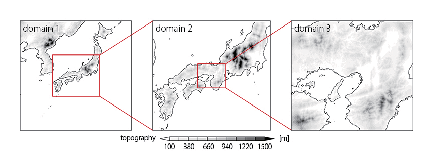
\includegraphics[width=1.0\hsize]{./figure/nesting_sample.eps}\\
  \caption{日本の近畿地方を対象領域としたドメインネスティング設定の例. domain 1が最外ドメインでdomain 3が最内ドメインである。
           赤い矩形と線は、それぞれの位置関係を示している。domain 1の水平格子間隔は7.5 km、domain 2は2.5 km、
           そしてdomain 3は0.5 kmである。}
  \label{fig_nestsample}
\end{center}
\end{figure}


\subsection{オフライン・ネスティング実験の方法} \label{sec:nest_offline}
%------------------------------------------------------

ここでは、親ドメインは解像度は荒いが広領域の外側ドメインで、子ドメインは領域は狭いが高解像度の内側ドメインで
あることを想定する。このとき、2段ネスティングのオフライン・ネスティング実験の実行過程は次のようになる。

{\gt
\begin{enumerate}
 \item 親ドメインの時間積分計算を行う。
 \item 親ドメインの出力ファイル(history)を用いて子ドメインの初期値/境界値を作成する。
 \item 作成した初期値/境界値を用いて子ドメインの時間積分計算を行う。
\end{enumerate}
}

以下、この流れに沿って説明を進める。親ドメインと子ドメインそれぞれについて、``pp.***.conf''、``init.***.conf''、
そして``run.***.conf''ファイルを事前に作成し、親ドメイン、子ドメインともに地形/土地利用データの作成を終え、
親ドメインについては、初期値/境界値データの作成を終えていることを想定して説明を進める。
ここで説明するオフライン・ネスティング実験の設定を記述したconfigファイルがチュートリアルディレクトリの下、
``tutorial/real/sample/offline\_nesting''に置いてあるので、説明を読み進める上で参考にしてもらいたい。

\subsubsection{親ドメインの時間積分計算を行う}
基本的には通常のシングルドメインの計算と同じ方法で実行すればよいが、``run.conf''ファイルの設定について、
次の5点の注意点・変更点がある。

\begin{itemize}
 \item 親ドメインのhistory出力間隔を適度に細かくとること。
 \item 親ドメインのhistory出力変数に必要なものが揃っているか確認すること。
 \item 親ドメインのhistory出力形式で\verb|ZINTERP|は``false''に設定すること。
 \item 親ドメインのhistory出力形式で\verb|STEP0|は``true''に設定すること。
 \item 親ドメインの計算領域を子ドメインへ伝える「カタログファイル」を出力すること。
\end{itemize}


この設定を``run.parent.conf''に適用すると下記のようになる。赤文字で示した部分が、
上記の注意点・変更点に対応する部分である。\\

\noindent {\small {\gt
\ovalbox{
\begin{tabularx}{140mm}{l}
\textcolor{red}{\verb|&PARAM_DOMAIN_CATALOGUE|} \\
\textcolor{red}{\verb| DOMAIN_CATALOGUE_OUTPUT = .true.,|} \\
\textcolor{red}{\verb|/|} \\
 \\
\verb|&PARAM_HISTORY| \\
\verb| HISTORY_DEFAULT_BASENAME  = "history",| \\
\textcolor{red}{\verb| HISTORY_DEFAULT_TINTERVAL = 600.D0,|} \\
\verb| HISTORY_DEFAULT_TUNIT     = "SEC",| \\
\verb| HISTORY_DEFAULT_TAVERAGE  = .false.,| \\
\verb| HISTORY_DEFAULT_DATATYPE  = "REAL4",| \\
\textcolor{red}{\verb| HISTORY_DEFAULT_ZINTERP   = .false.,|} \\
\textcolor{red}{\verb| HISTORY_OUTPUT_STEP0      = .true.,|} \\
\verb|/| \\
\end{tabularx}
}}}\\

\verb|PARAM_DOMAIN_CATALOGUE|の項目の``\verb|DOMAIN_CATALOGUE_OUTPUT|''の変数がカタログファイルの出力設定である。
もともとのconfigファイルには項目自体がないこともあるので、その場合は自分で項目を加えて設定すること。
カタログファイルは、``latlon\_domain\_catalogue.txt''というファイル名で出力される。この中には、MPIプロセス毎に分割
して担当した計算領域の四隅の緯度・経度が記述されている。

\verb|HISTORY_DEFAULT_TINTERVAL|の設定項目によってhistoryデータ出力間隔を指定する(単位は秒である)。指定値に
任意性はあるが、子ドメインの側面境界条件の更新間隔として使用可能であると考えられる範囲で指定すること。
親ドメイン、子ドメインの解像度、および実行環境のディスク空き容量にもよるが、おおよそ最大で1時間間隔、
出来れば10分間隔のhistoryデータ出力間隔を指定することが多い。

また、historyデータを用いて初期値/境界値データを作成するために、
下記の全ての変数を出力する必要がある。
run.confファイルの``HISTITEM''の項目を確認すること。

\begin{itemize}
 \item \verb|T2, Q2, MSLP, DENS, MOMZ, MOMX, MOMY, RHOT|
 \item \verb|QV, QC, QR, QI, QS, QG| {\small (親の雲微物理モデルに合わせて出力; 例えばTomita08なら全て)}
 \item \verb|NC, NR, NI, NS, NG| {\small (親の雲微物理モデルに合わせて出力; 例えばTomita08なら不要)}
 \item \verb|LAND_SFC_TEMP, URBAN_SFC_TEMP, OCEAN_SFC_TEMP|
 \item \verb|OCEAN_ALB_LW, OCEAN_ALB_SW, LAND_ALB_LW, LAND_ALB_SW|
 \item \verb|OCEAN_TEMP, OCEAN_SFC_Z0M, LAND_TEMP, LAND_WATER|
\end{itemize}

設定が完了すれば、``scale-rm''を実行して親ドメインの時間積分計算を行う。


\subsubsection{親ドメインの出力ファイルを用いて子ドメインの初期値/境界値を作成する}
次に計算が終わった親ドメインのhistoryデータ出力を用いて、子ドメインの初期値/境界値を作成する。
実行するプログラムは、通常の初期値/境界値作成と同じ``scale-rm\_init''だが、
``init.child.conf''を下記のように編集する。\\

\noindent {\small {\gt
\ovalbox{
\begin{tabularx}{140mm}{l}
\verb|&PARAM_MKINIT_REAL| \\
\verb| BASENAME_BOUNDARY   = "boundary",| \\
\textcolor{red}{\verb| BASENAME_ORG        = "history",|} \\
\textcolor{red}{\verb| FILETYPE_ORG        = "SCALE-RM",|} \\
\textcolor{red}{\verb| NUMBER_OF_TSTEPS    = 25,|} \\
\textcolor{red}{\verb| BOUNDARY_UPDATE_DT  = 600.D0,|} \\
\verb|/| \\
 \\
\textcolor{red}{\verb|&PARAM_NEST|} \\
\textcolor{red}{\verb| USE_NESTING               = .true.,|} \\
\textcolor{red}{\verb| OFFLINE                   = .true.,|} \\
\textcolor{red}{\verb| OFFLINE_PARENT_PRC_NUM_X  = 4,|} \\
\textcolor{red}{\verb| OFFLINE_PARENT_PRC_NUM_Y  = 4,|} \\
\textcolor{red}{\verb| OFFLINE_PARENT_KMAX       = 35,|} \\
\textcolor{red}{\verb| OFFLINE_PARENT_IMAX       = 40,|} \\
\textcolor{red}{\verb| OFFLINE_PARENT_JMAX       = 40,|} \\
\textcolor{red}{\verb| OFFLINE_PARENT_LKMAX      = 5,|} \\
\textcolor{red}{\verb| LATLON_CATALOGUE_FNAME    = "latlon_domain_catalogue.txt",|} \\
\textcolor{red}{\verb|/|} \\
\end{tabularx}
}}}\\

\noindent 読み込む外部入力データのファイル名を指定する``\verb|BASENAME_ORG|''は、親モデルのhistory.pe***.nc
ファイルを読み込むので、``history''と指定する。また、このhistoryファイルはSCALE-RMモデルの出力データなので、
``\verb|FILETYPE_ORG|''は、``SCALE-RM''と指定する。\verb|NUMBER_OF_TSTEPS|には、historyファイルが持つ時間ステップ数
を記述する(例として25が記述されているだけ)。\verb|BOUNDARY_UPDATE_DT|には、時間ステップの時間間隔を指定する
(単位は秒である)。つまり、親ドメインの\verb|HISTORY_DEFAULT_TINTERVAL|の設定項目に一致する値を指定する。
この説明では、親ドメインで600秒としたので、ここでも600秒を指定する。

\verb|PARAM_NEST|の項目は、ネスティング実験のために新たに加える項目である。もともとのconfigファイルには項目自体がないので、
自分でconfigファイルに追記する。最初の2つの項目によって、オフライン・ネスティング実験であることが決定される。
``\verb|OFFLINE_PARENT_|''で始まる6つの設定変数は、親ドメインの設定を記述する変数である。親ドメインの対応する項目を
参照して正しく設定すること。この例では、親ドメインは$4 \times 4$のMPIプロセス数を使用し、鉛直35層で、水平には1つの
MPIプロセスあたり$40 \times 40$の格子点を持っており、陸面モデルは5層モデルであることを想定している。
最後の``\verb|LATLON_CATALOGUE_FNAME|''の項目は、親ドメインを実行した時に出力したカタログファイルを指定する。

設定の編集が完了すれば、``scale-rm\_init''を実行して子ドメインの初期値/境界値を作成する。\\

\noindent {\small {\gt
\fbox{
\begin{tabularx}{140mm}{l}
\verb|xxx ERROR: REQUESTED DOMAIN IS TOO MUCH BROAD| \\
\verb|xxx -- LONGITUDINAL direction over the limit| \\
\end{tabularx}
}}}\\

\noindent 実行時に上記のようなメッセージが表示されて計算が止まる場合は、子ドメインの計算領域が親ドメインの計算領域の
外側に取られている部分がある。この場合は、各ドメインの大きさや領域中心の設定を見直す必要がある。


\subsubsection{作成した初期値/境界値を用いて子ドメインの時間積分計算を行う}
初期値/境界値作成が終われば、子ドメインの時間積分計算を実行する。子ドメインの実行は、通常の現実大気実験と何も変わらないので、
必要なデータのPATHが正しくconfigファイルに記述されていることを確認してから、``scale-rm''を実行すればよい。

1点だけ忘れやすい設定項目を挙げておく。\\

\noindent {\small {\gt
\ovalbox{
\begin{tabularx}{140mm}{l}
\verb|&PARAM_MKINIT_REAL| \\
\verb|     〜 中略 〜|\\
\textcolor{red}{\verb| BOUNDARY_UPDATE_DT  = 600.D0,|} \\
\verb|/| \\
\end{tabularx}
}}}\\

\noindent ``run.child.conf''の\verb|BOUNDARY_UPDATE_DT|を、初期値/境界値作成で使用した親ドメインの
historyデータ出力間隔に合わせておくことを忘れないようにすること。オフライン・ネスティング実験の場合、
現在のところこの設定に親ドメインと子ドメイン間で不整合あっても警告やエラーメッセージが発せられないまま、
時間積分計算が進み、場合によっては正常終了してしまうため注意が必要である。

多段のオフライン・ネスティング実験を行いたい場合は、ここまでの過程を繰り返せばよい。つまり、子ドメインとして
時間積分計算した結果を再度、親ドメインと見立てて、さらに内側の孫ドメインの初期値/境界値作成を行なえばよい。
以上でオフライン・ネスティングの実行方法の説明を終える。


\subsection{オンライン・ネスティング実験の方法} \label{sec:nest_online}
%------------------------------------------------------

オフライン・ネスティング実験では、各ドメインの計算を逐次的に実行する必要があったが、オンライン・ネスティング実験では
全てのドメインの計算を同時に実行する。現在は、親ドメインから子ドメインへのみデータ受け渡しを行う、いわゆる
``1-Wayネスティング''のみをサポートしている。オンライン・ネスティング実験でサポートするネスティング段数は、
最大で10段までである。

SCALEのオンライン・ネスティング実験は、複数のドメインを逐次的に時間積分計算を進めるのではなく、並列的に時間積分計算を行う。
図\ref{fig_mpisplit}に示すイメージ図のように、与えられたMPIプロセスを分割してそれぞれのドメインに分配し、各々のドメインが
独立したモデルのように計算を進める。後ほど説明するが、複数のドメインを立ち上げるために実行時には``launch.conf''という
起動用のconfigファイルが別途必要になる。

\begin{figure}[t]
\begin{center}
  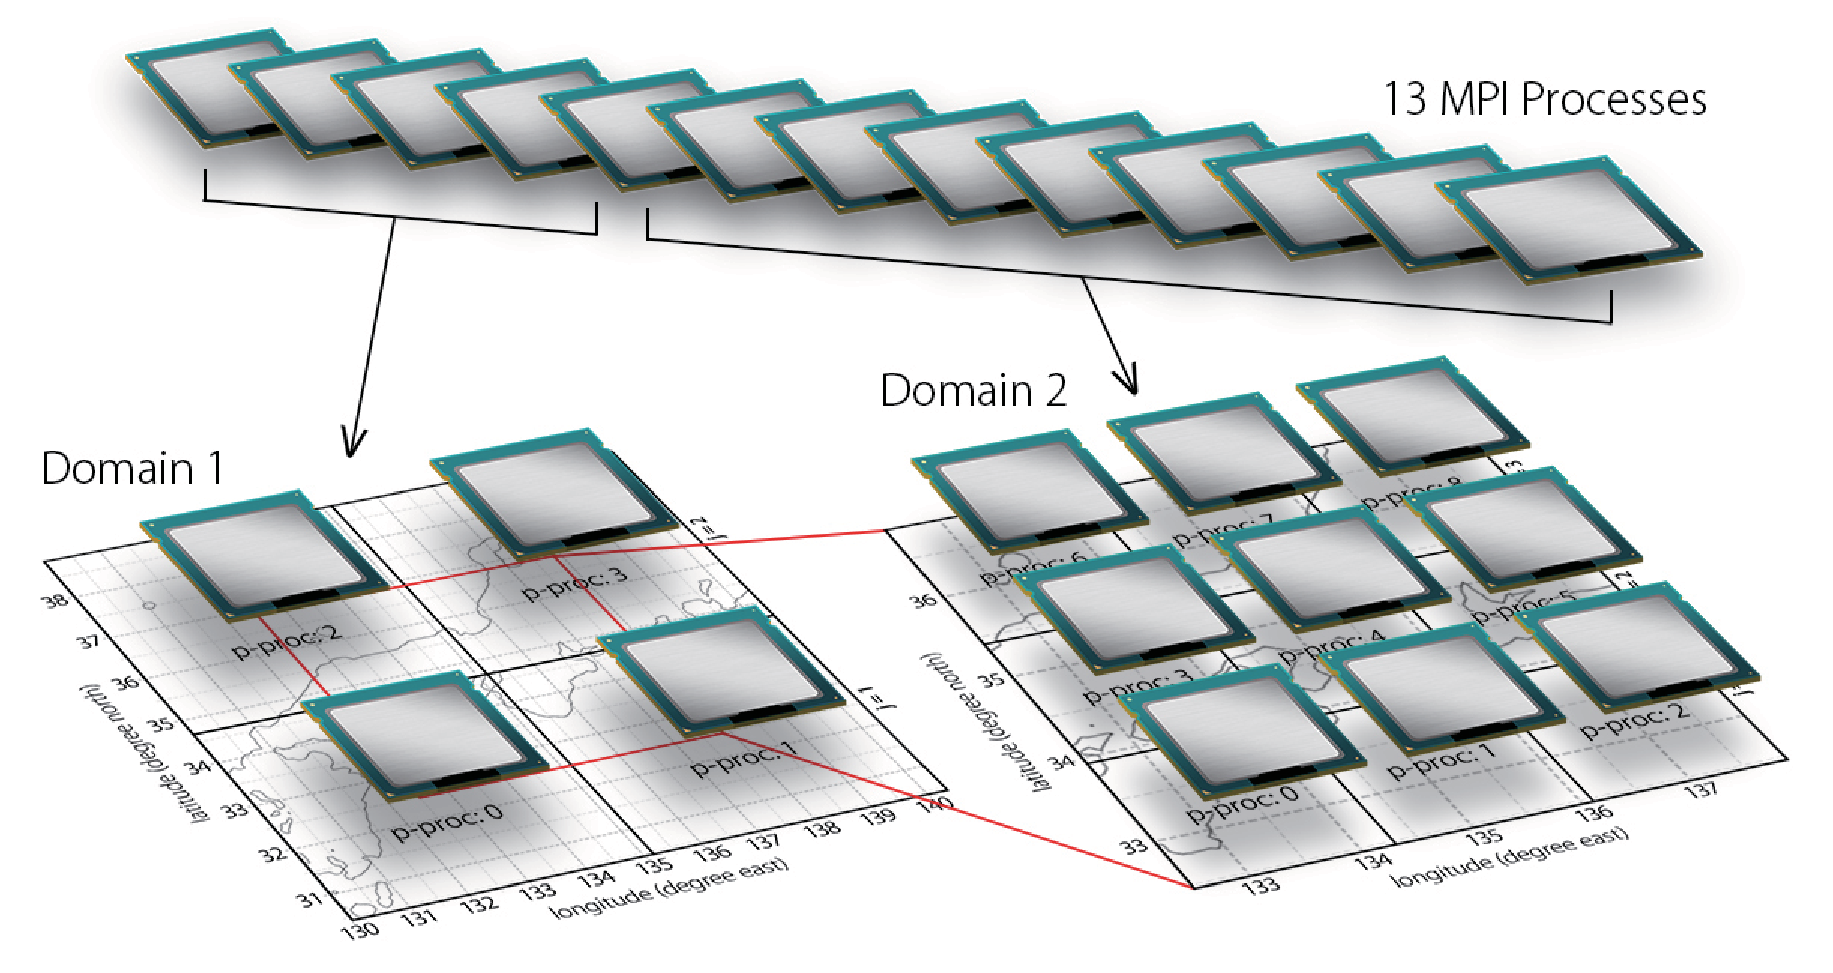
\includegraphics[width=0.8\hsize]{./figure/mpisplit_nesting.eps}\\
  \caption{オンライン・ネスティング実験のMPIプロセス配分イメージ. 全部で13のプロセスを立ち上げ、これを適切に分配することで、
           Domain 1は$2 \times 2$の4-MPI並列、Domain 2は$3 \times 3$の9-MPI並列計算を行う。Domain 1からDomain 2へMPI通信
           によってデータを受け渡ししながら時間積分計算を進める。}
  \label{fig_mpisplit}
\end{center}
\end{figure}


ここでは、最も単純な2段ネスティングの例を説明する。親ドメインは解像度は荒いが広領域の外側ドメインで、
子ドメインは領域は狭いが高解像度の内側ドメインであることを想定する。

オンライン・ネスティング実験を行う場合は、``scale-rm''のモデル本体実行前に全てのドメインについて、
地形/土地利用データの作成、及び初期値/境界値データの作成を事前に行っておく必要がある。従って、親ドメインと子ドメイン
それぞれについて、``pp.***.conf''、``init.***.conf''、そして``run.***.conf''ファイルを事前に作成し、
親ドメイン、子ドメインともに地形/土地利用データの作成、及び初期値/境界値データの作成を終えていることを想定して説明を進める。
ここで説明するオンライン・ネスティング実験の設定を記述したconfigファイルがチュートリアルディレクトリの下、
``tutorial/real/sample/online\_nesting''に置いてあるので、説明を読み進める上で参考にしてもらいたい。


\subsubsection{configファイルの編集}
まず、親ドメイン、子ドメインそれぞれに``run.***.conf''ファイルを編集する。

\noindent {\gt \verb|run.parent.conf|の編集内容}\\
{\small {\gt
\ovalbox{
\begin{tabularx}{140mm}{l}
\verb|&PARAM_NEST| \\
\verb| USE_NESTING              = .true.,| \\
\verb| OFFLINE                  = .false.,| \\
\verb| ONLINE_DOMAIN_NUM        = 1,| \\
\verb| ONLINE_IAM_PARENT        = .true.,| \\
\verb| ONLINE_IAM_DAUGHTER      = .false.,| \\
\verb| ONLINE_BOUNDARY_USE_QHYD = .true.,| \\
\verb| ONLINE_AGGRESSIVE_COMM   = .true.,| \\
\verb|/| \\
\end{tabularx}
}}}\\

\vspace{0.5cm}

\noindent {\gt \verb|run.child.conf|の編集内容}\\
{\small {\gt
\ovalbox{
\begin{tabularx}{140mm}{l}
\verb|&PARAM_NEST| \\
\verb| USE_NESTING              = .true.,| \\
\verb| OFFLINE                  = .false.,| \\
\verb| ONLINE_DOMAIN_NUM        = 2,| \\
\verb| ONLINE_IAM_PARENT        = .false.,| \\
\verb| ONLINE_IAM_DAUGHTER      = .true.,| \\
\verb| ONLINE_BOUNDARY_USE_QHYD = .true.,| \\
\verb| ONLINE_AGGRESSIVE_COMM   = .true.,| \\
\verb|/| \\
\end{tabularx}
}}}\\

\noindent 上記の\verb|PARAM_NEST|の項目は、ネスティング実験のために新たに加える項目である。
もともとのconfigファイルには項目自体がないので、自分でconfigファイルに追記する。最初の2つの項目によって、
オンライン・ネスティング実験であることが決定される。``\verb| ONLINE_|''で始まる設定変数はオンライン・ネスティング実験
専用の設定変数である。\verb|ONLINE_DOMAIN_NUM|は、ドメインのID番号であり、外側ドメインから内側ドメインへ順番に
番号を振っていく。ここでは、親ドメインは1番、子ドメインは2番と設定する。

\verb|ONLINE_IAM_PARENT|と\verb|ONLINE_IAM_DAUGHTER|は各ドメインの役割を設定するパラメータである。
これらの変数は、``In online nesting system, I am parent (or, I am child).''という意味で覚えれば設定を間違うことはない。
少し脇道にそれるが、ここで説明している設定より複雑なものとして、図\ref{fig_nestsample}のような
3段ネスティング実験の場合の設定例を表\ref{tab:triple_nested}に示した。

\begin{table}[htb]
\begin{center}
\caption{3段ネスティング実験の設定例}
\begin{tabularx}{150mm}{|l|l|l|X|} \hline
 \rowcolor[gray]{0.9} ドメイン & \verb|ONLINE_DOMAIN_NUM| & \verb|ONLINE_IAM_PARENT| & \verb|ONLINE_IAM_CHILD|\\ \hline
 最外ドメイン & 1 & \textcolor{blue}{true} & \textcolor{red}{false} \\ \hline
 中間ドメイン & 2 & \textcolor{blue}{true} & \textcolor{blue}{true} \\ \hline
 最内ドメイン & 3 & \textcolor{red}{false} & \textcolor{blue}{true} \\ \hline
\end{tabularx}
\label{tab:triple_nested}
\end{center}
\end{table}

\noindent 最外ドメインは親ドメインとしてのみ働き、最内ドメインは子ドメインとしてのみ働く。一方、中間ドメインは最外ドメインに
対しては子ドメイン、最内ドメインに対しては親ドメインとして働くため両方共``true''となる。

さて、configファイルの編集内容の説明に戻る。\verb|ONLINE_BOUNDARY_USE_QHYD|は、「側面境界条件として親ドメインの凝結物の
混合比を使うかどうか」を指定する設定変数である。外部入力データから側面境界条件を作成するときには通常使わないが、
ネスティングの場合、ドメイン間の物理スキームの違いがなかったり、解像度もそれほど大きく離れていないため、側面境界から
凝結物自体が移流して入ってくる設定も選択肢に入るだろう。側面境界付近で雲が立ちにくい問題を解決したり、親ドメインとの乖離を
抑制したりする可能性がある。

最後の\verb|ONLINE_AGGRESSIVE_COMM|はオンライン・ネスティング時のドメイン間通信に関する最適化変数である。
通常は、``true''と設定して実行する。


\subsubsection{launchファイルの編集}
オンライン・ネスティング実験の実行には、``run.***.conf''の他に、起動用configファイル``launch.conf''が必要である。
\begin{verbatim}
 $ vi launch.conf
\end{verbatim}
などとして、適宜エディタをたちあげて新規ファイルを作成し、下記の内容を記述する。\\

\noindent {\small {\gt
\ovalbox{
\begin{tabularx}{140mm}{l}
\verb|&PARAM_LAUNCHER| \\
\verb| NUM_DOMAIN  = 2,| \\
\verb| CONF_FILES  = run.parent.conf,run.child.conf,| \\
\verb| PRC_DOMAINS = 4,9,| \\
\verb|/| \\
\end{tabularx}
}}}\\

\noindent 図\ref{fig_mpisplit}のイメージを思い浮かべながら設定を確認してもらいたい。\verb|PARAM_LAUNCHER|の項目のうち、
\verb|NUM_DOMAIN = 2|が「2つのドメインを起動する」ことを表しており、\verb|CONF_FILES|の項目に羅列されたファイル名は、
各々のドメインで読み込むconfigファイルを指定している。\verb|PRC_DOMAINS|は各々のドメインで使用するMPIプロセス数を
指定する。\verb|PRC_DOMAINS|は、\verb|CONF_FILES|で羅列した順番で指定しなければならない。従ってこの場合、
親ドメインは4-MPI並列、子ドメインは9-MPI並列で実行するように指定されている。ここで指定するMPIプロセス数は、
各々の``run.***.conf''で指定されている総MPIプロセス数と合致させなければならない。
この2段オンライン・ネスティング実験で使用する総MPIプロセス数は、$4 + 9 = 13$プロセスとなる。

実行時には、シングルドメイン計算とは異なり、\verb|launch.conf|を引数に指定し、計算全体で使用するMPIプロセス数を
指定して実行する。
\begin{verbatim}
 $ mpirun  -n  13  ./scale-rm  launch.conf
\end{verbatim}

実行にあたって注意することは、複数のドメインの計算を同時に実行するため、\textcolor{red}{ドメイン間でconfigファイルに
記述された出力ファイル名をドメイン毎に変更しなければならない}ことである。たとえば,``history.pe***.nc''は、
``history\_d01.pe***.nc''、``history\_d02.pe***.nc''といったようにドメイン毎に名前を変えながらどのドメインの
出力データであるか判別がつくようにconfigファイルの記述を設定する。
historyファイルのほかに、LOGファイル、topoファイル、landuseファイル、boundaryファイル、initファイル、restartファイル、
そしてmonitorファイルの名前を変更しておく必要がある。

実行時に次のようなエラーメッセージが出力されて計算が異常終了することがある。\\

\noindent {\small {\gt
\fbox{
\begin{tabularx}{140mm}{l}
\verb|xxx region of daughter domain is larger than that of parent: SW search| \\
\end{tabularx}
}}}\\

\noindent {\small {\gt
\fbox{
\begin{tabularx}{140mm}{l}
\verb|xxx region of daughter domain is larger than that of parent: NE search| \\
\end{tabularx}
}}}\\

\noindent これは、子ドメインで設定された計算領域が親ドメインの計算領域よりも大きいことを意味するエラーメッセージである。
``SW search''のエラーが出る場合は子ドメインの西側か南側が親ドメインの外側に出ており、``NE search''のエラーが出る場合は
子ドメインの東側か北側が親ドメインの外側に出ていることを意味している。再度設定を確認し、地形・土地利用データ、および
初期値/境界値作成からやり直すこと。


\subsubsection{MPIプロセスの分配ガイドライン}
SCALEのオンライン・ネスティング実験は、図\ref{fig_mpisplit}のイメージ図で説明したように、MPIプロセスを分割し、複数のドメイン
に分配する。現在のところ、その分配割合はユーザーに委ねられているため、適切にMPIプロセスを分配しなければ余計な計算時間が
かかってしまう。ここでは、適切にMPIプロセスを分配するためのガイドラインについて説明する。ガイドラインは、ドメイン毎に
\textcolor{blue}{「単位あたりの時間積分にかかる1プロセスあたりの演算量を揃える」}という単純なものである。
ここでは、以下に示す2段オンライン・ネスティング実験を行う場合を想定し、ガイドラインに沿ったプロセス分配方法の例を示す。
``domain 1''は外側の親ドメイン、``domain 2''は内側の子ドメインを意味する。

\begin{table}[htb]
\begin{center}
\caption{2段オンライン・ネスティング実験の設定想定}
\begin{tabularx}{150mm}{|l|l|X|} \hline
 \rowcolor[gray]{0.9} 設定項目 & domain 1 & domain 2 \\ \hline
 計算領域 & 450 km $\times$ 450 km & 200 km $\times$ 200 km \\ \hline
 DX \& DY(X,Y同一設定) & 3 km & 1 km \\ \hline
 鉛直層設定 & 40層 & 60層 \\ \hline
 積分時間間隔(DT)& 30 sec & 10 sec \\ \hline
 積分時間 & 3600 sec & 3600 sec \\ \hline
\end{tabularx}
\label{tab:nest_proc_guide1}
\end{center}
\end{table}

このとき、親ドメインの水平方向の一辺の格子点数は、$450 km \div 3 km = 150$点であるので、総格子点数は
$X \times Y \times Z = 150 \times 150 \times 40 = 900,000$点である。一方、子ドメインの水平方向の一辺の格子点数は、
$200 km \div 1 km = 200$点であるので、総格子点数は$200 \times 200 \times 60 = 2,400,000$点である。1つの時間ステップの
積分を行うのにこれだけの格子点について計算を行わなければならない。

積分時間間隔は格子間隔に依存するためにドメイン毎に異なる。この例では、domain 1は30 secだが、domain 2は10 secであり、
3倍の差がある。したがって、同じ30 secという積分時間に対してdomain 2は3倍多くの時間ステップ、つまり3倍の演算量を要する。
これらを考慮して、簡単なドメイン間の演算量比率(Computation Rate)の指標を考えると下記の式で表される。
\begin{eqnarray}
ComputationRate=\frac{Xgrd_{child} \times Ygrd_{child} \times Zgrd_{child} \times Ustep_{child}}
                     {Xgrd_{parent} \times Ygrd_{parent} \times Zgrd_{parent} \times Ustep_{parent}} \nonumber
\end{eqnarray}
ここで、Xgrd、Ygrd、ZgrdはそれぞれX方向、Y方向、Z方向の格子点数を表し、Ustepは単位時間積分に必要な時間ステップ数を表す。
ここでの例をこの式に当てはまると、演算量比率は$(2,400,000 \times 3) \div (900,000 \times 1) = 8$であることがわかる。
おおよそ、この割合にしたがってMPIプロセスをドメイン毎に分配すればよい。例えばdomain 1は4プロセス、domain 2は32プロセスを
使用し、全体で36プロセスを使用する設定が考えられる。この場合、例えば次のように設定することができる。

\begin{table}[htb]
\begin{center}
\caption{2段オンライン・ネスティング実験のMPIプロセス設定例}
\begin{tabularx}{150mm}{|l|l|X|} \hline
 \rowcolor[gray]{0.9} 設定項目 & domain 1 & domain 2 \\ \hline
 MPIプロセス(X $\times$ Y) & 2 $\times$ 2 & 4 $\times$ 8 \\ \hline
 水平格子点数(IMAX $\times$ JMAX) & 75 $\times$ 75 & 50 $\times$ 25 \\ \hline
\end{tabularx}
\label{tab:nest_proc_guide2}
\end{center}
\end{table}

X方向とY方向に分配するプロセス数には任意性が残るが、この例のdomain 2のようにXとYで大きくプロセス数が異なる場合には、
X方向の格子点数(IMAX)の値が大きくなる設定を取ると計算機の演算性能を引き出しやすいと考えられる\footnote{SCALEでは
X方向のDo Loopが最も最内ループになっているため、X方向の回転数が多いとプリフェッチ機能が効果を発揮しやすく、メモリ性能
へのプレッシャーが緩和される。ただし、京の場合のようにスレッド並列も併用するハイブリッド並列の場合にはY方向の格子点数
もある程度大きくしてスレッド間の演算量のインバランスを小さくする必要性も出てくる。}。

この設定は一例であり、これ以外の方法で設定しても構わない。また、ここでは格子点数と積分時間間隔だけに着目して演算量比率
を考えたが、実際の計算には様々な物理過程も含まれるだろうし、それらをCallする時間間隔もドメイン毎に異なるかもしれない。
さらにドメイン内通信やドメイン間通信のMPI通信にかかる時間も影響を及ぼす。SCALEにおけるオンライン・ネスティングの実装に
おいて最も重要なことは、最内ドメインが時間積分を実行し続けることである。同じ設定で何度も実験を行うような場合には、上記の
方法である程度の見通しをつけた上で、いくらかの微調整を行うことをおすすめする。
以上でオンライン・ネスティングの実行方法の説明を終える。


\subsection{子ドメインにおける地形の取り扱い} \label{sec:nest_topo}
%------------------------------------------------------
ネスティング実験を行う際、ドメイン間の格子間隔比率が大きい場合などに子ドメインのバッファー領域内で不整合が発生する
可能性がある。バッファー領域内は親ドメインの計算結果を用いて一部の変数にダンピングがかかるが、地形の表現性が異なる
ことで、子ドメインにとっては正しくない値へダンピングされる可能性がある。例えば、子ドメインでは斜面上の小さな谷として
表現されている地形が、親ドメインでは格子間隔が荒く谷がなくスムースな斜面として表現される場合が考えられる。

こういった不整合を無くすために、バッファー領域では親ドメインの地形を用い、内側領域では子ドメイン自身の地形を用いる
「地形コピー」の機能が実装されている。この機能を使えば、図\ref{fig_topocopy}に示すようにバッファー領域は完全に
親ドメインに一致する地形で、内側に移る地形遷移領域内では親ドメインと子ドメインのミックス、それより内側では完全に
子ドメインの地形という設定を構築することができる。以降、その設定方法と実行手順を説明する。基本的には、
オフライン・ネスティングのフレームワークを利用して進める。
ここで説明する地形コピーの設定を記述した``pp.d0*.conf''ファイルがチュートリアルディレクトリの下、
``tutorial/real/sample/online\_nesting''に置いてあるので、説明を読み進める上で参考にしてもらいたい。

\begin{figure}[tb]
\begin{center}
  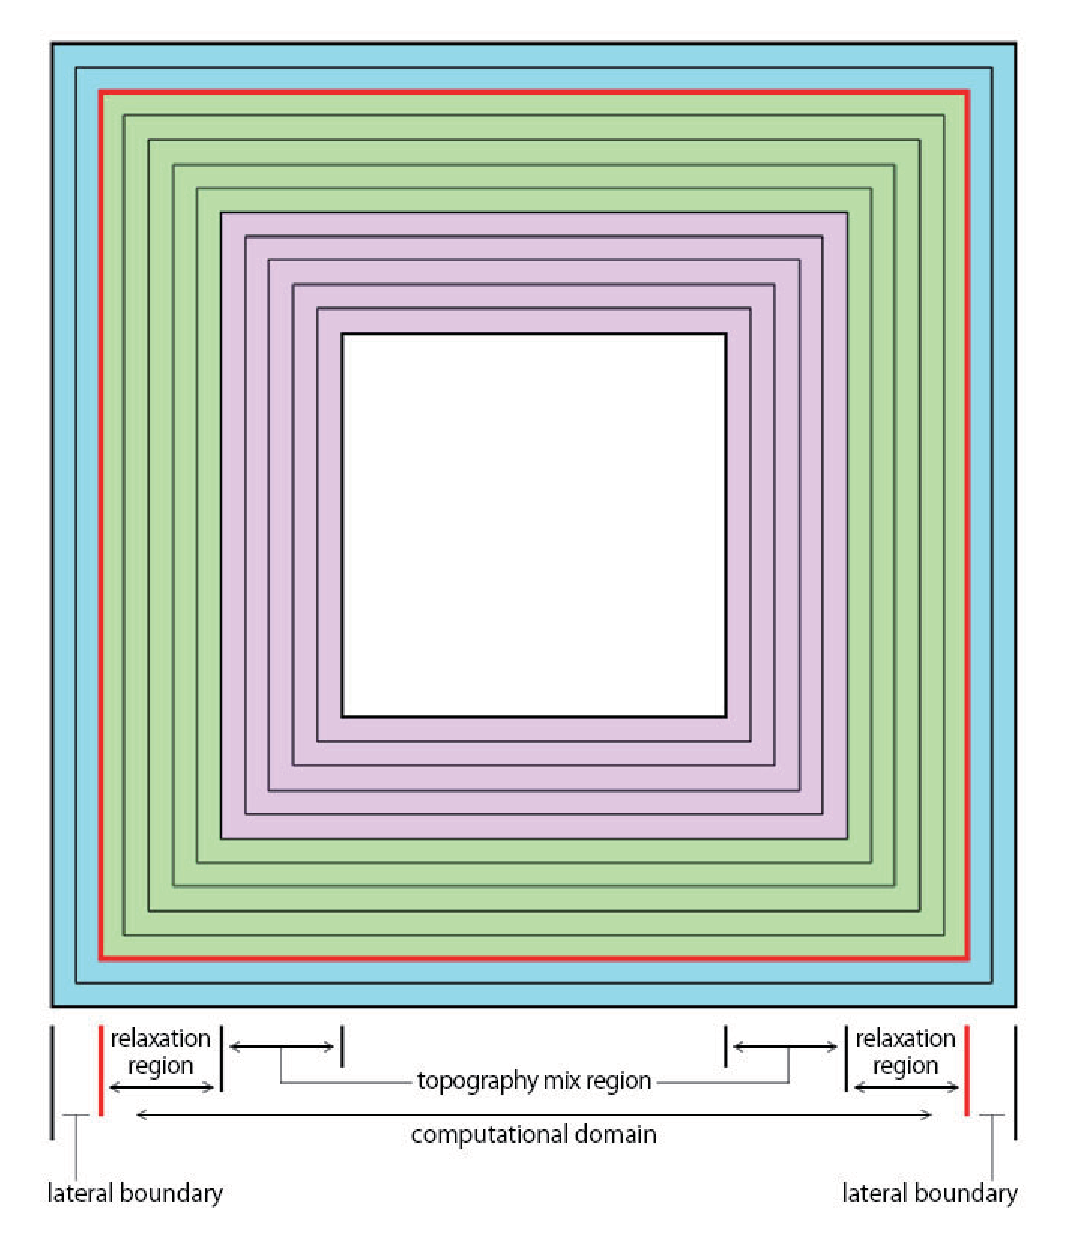
\includegraphics[width=0.4\hsize]{./figure/topo_copy.eps}\\
  \caption{地形コピーを適用した子ドメインの地形データ水平分布. 最外の水色の2層は側面境界で、それより内側の赤色の線で
           囲われた領域が計算領域である。緑色の部分がバッファー領域、桃色の部分が地形遷移領域、そして最内の白色の
           部分が子ドメインの地形をもつ領域である。地形遷移領域では外側から内側にかけて徐々に親ドメインの地形データから
           子ドメインの地形データへ遷移する。}
  \label{fig_topocopy}
\end{center}
\end{figure}

まず親ドメインの``pp.d01.conf''ファイルを編集して、計算領域の大きさを子ドメインへ伝えるために緯度経度カタログ
ファイルを出力するように設定する。具体的には、下記の記述を``pp.d01.conf''ファイルに追記する。\\

\noindent {\small {\gt
\ovalbox{
\begin{tabularx}{140mm}{l}
\verb|&PARAM_DOMAIN_CATALOGUE| \\
\verb| DOMAIN_CATALOGUE_FNAME  = "latlon_domain_catalogue.txt",| \\
\verb| DOMAIN_CATALOGUE_OUTPUT = .true.,| \\
\verb|/| \\
\end{tabularx}
}}}\\

\noindent その他の設定項目は通常通りで良い。編集ができたら親ドメインの地形データ作成を実行する(つまり、
scale-rm\_ppを実行する)。ここで、出力データは、``topo\_d01.pe***.nc''というファイル名で保存されていると
想定する。次に、子ドメインの``pp.d02.conf''ファイルを編集する。\\

\noindent {\small {\gt
\ovalbox{
\begin{tabularx}{140mm}{l}
\verb|&PARAM_CNVTOPO| \\
\verb|     〜 中略 〜|\\
\verb| CNVTOPO_copy_parent     = .true.,| \\
\verb|/| \\
 \\
\verb|&PARAM_COPYTOPO| \\
\verb| COPYTOPO_IN_BASENAME   = "topo_d01",| \\
\verb| COPYTOPO_ENTIRE_REGION = .false.,| \\
\verb| COPYTOPO_LINEAR_H      = .true.,| \\
\verb|/| \\
 \\
\verb|&PARAM_NEST| \\
\verb| USE_NESTING               = .true.,| \\
\verb| OFFLINE                   = .true.,| \\
\verb| OFFLINE_PARENT_PRC_NUM_X  = 4,| \\
\verb| OFFLINE_PARENT_PRC_NUM_Y  = 4,| \\
\verb| OFFLINE_PARENT_KMAX       = 35,| \\
\verb| OFFLINE_PARENT_IMAX       = 40,| \\
\verb| OFFLINE_PARENT_JMAX       = 40,| \\
\verb| OFFLINE_PARENT_LKMAX      = 5,| \\
\verb| LATLON_CATALOGUE_FNAME    = "latlon_domain_catalogue.txt",| \\
\verb|/| \\
\end{tabularx}
}}}\\

\noindent もともとconfigファイルにある\verb|PARAM_CNVTOPO|の項目に、\verb|CNVTOPO_copy_parent = .true.|
という記述を加える。これは地形コピーの実行を指示するスイッチである。
次の\verb|PARAM_COPYTOPO|は、地形コピーの設定項目群であり、すべて追記すること。
1つ目の\verb|COPYTOPO_IN_BASENAME|は、親ドメインの地形データのPATHを指定する。ここでは、親ドメインの
出力データは``topo\_d01.pe***.nc''というファイル名でカレントディレクトリに保存されていると指定している。
2つ目の\verb|COPYTOPO_ENTIRE_REGION|は、全領域でコピーするかどうかを決定するオプションである。
このスイッチをtrueにすると、図\ref{fig_topocopy}に示された桃色と白色の領域は無くなり、全て緑色の
完全コピー領域になる。3つ目の\verb|COPYTOPO_LINEAR_H|は、地形遷移領域の遷移具合を調整するスイッチである。
\verb|COPYTOPO_LINEAR_H|がtrueだと線形プロファイルで遷移し、falseだと指数関数プロファイルで遷移する。

地形遷移領域の幅は、デフォルト設定ではバッファー領域と同じ幅になる。バッファー領域の設定と同じ要領で、
\verb|COPYTOPO_TRANSITION_DX|、\verb|COPYTOPO_TRANSITION_DY|、および\verb|COPYTOPO_TRANSFACT|の
変数を使って任意の幅に設定することができる。

最後の\verb|PARAM_NEST|の項目はオフライン・ネスティング実験のフレームワークを利用するための設定項目であり、
全て追記する必要がある。設定変数の詳しい説明は、\ref{sec:nest_offline}節のオフライン・ネスティング実験の説明を
参照してほしい。

configファイルの編集が終われば、子ドメインの地形データ作成を実行する。3つ以上のドメインがある場合は、
上記の実行過程を外側ドメインから順に繰り返せばよい。



\section{複数の実験を一括実行する:バルクジョブ機能} \label{sec:bulkjob}
%====================================================================================

SCALEには「一括実行機能」、いわゆるバルクジョブ機能が備わっている。これは、パラメタスイープ実験、
初期値アンサンブル実験や、Time Slice気候実験など多数の実験を行う場合に便利な機能である。SCALEモデル本体の実行は
もちろん、ドメインネスティング実験の場合でも利用できるし、地形・土地利用データ作成(地形コピーを利用しない場合のみ)、
初期値/境界値作成、そして後処理ツールのnet2g(netcdf2grads\_bulkを使用)にも適用可能である。
各プログラムの実行内容は異なっていても構わないが、MPI並列としての構造は共通していなければならない点に注意すること。
1つの計算事例をここでは「ジョブ」と呼ぶこととする。以下では、3つの2段オンライン・ネスティング実験を一括に行う例を
もとに説明する(積分期間、もしくは計算領域中心が異なっている3つのジョブを想定している)。


\begin{figure}[t]
\begin{center}
  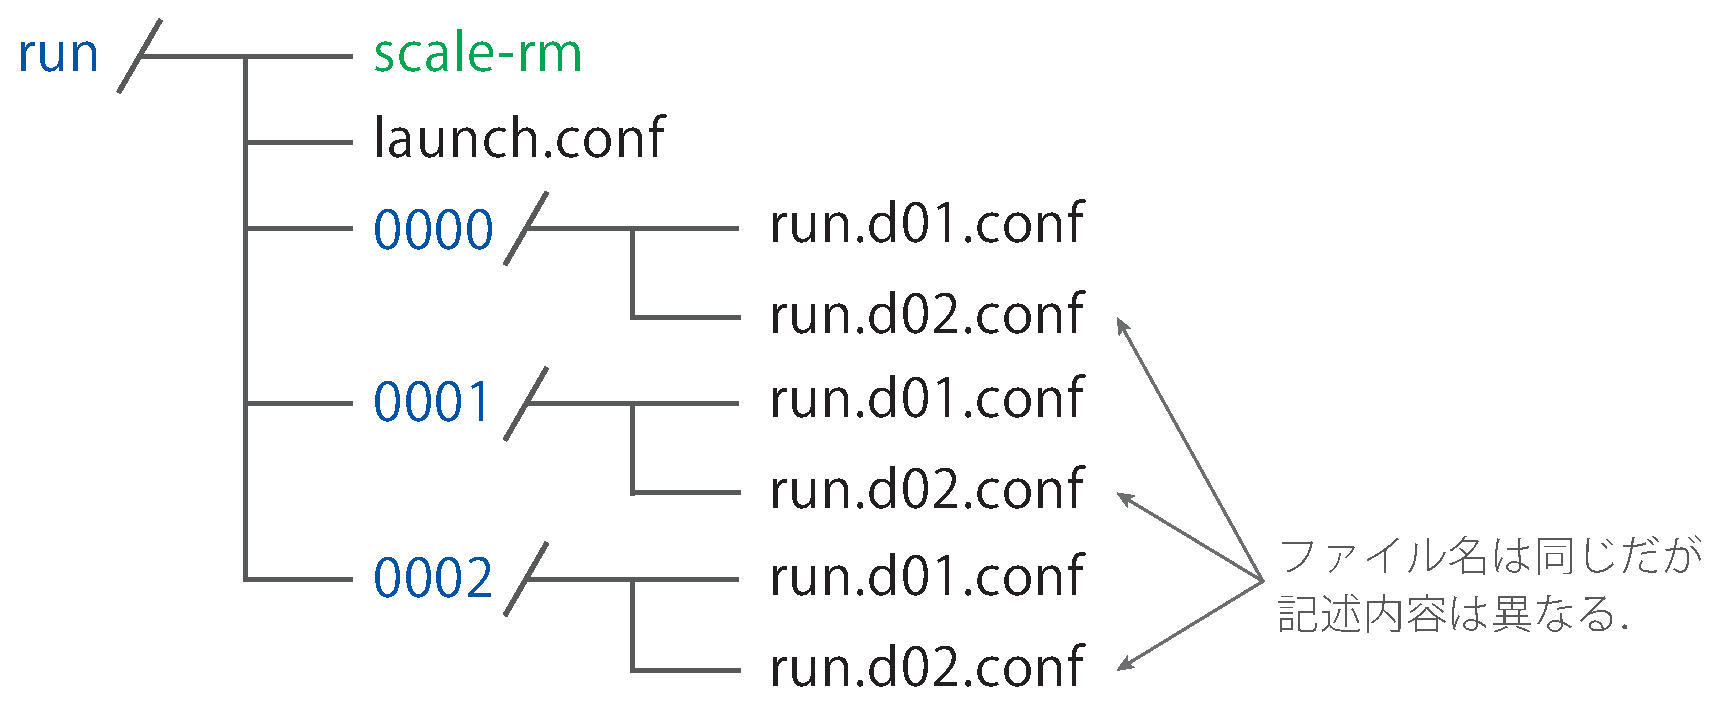
\includegraphics[width=0.6\hsize]{./figure/bulkjob_directory_structure.eps}\\
  \caption{バルクジョブ機能を使ってscale-rmを実行する場合のディレクトリ構造. ``0000''や``0001''はジョブ番号
           に対応する名前を持ったジョブディレクトリである。各ジョブディレクトリの中には、そこで実行する実験に関する
           configファイルが置かれている。データパラメタテーブルなどのファイルやディレクトリの記述は割愛しているが、
           それらも必要に応じて適切に配置する必要がある。}
  \label{fig_bulkjob}
\end{center}
\end{figure}


バルクジョブ実行するにあたって下記のものを事前に準備する必要がある。
\begin{itemize}
\item バルクジョブ用のディレクトリ構造
\item 実験に必要なすべてのconfigファイル
\item 実験に必要なすべての外部入力データ
\item 実行用のlaunch.confファイル
\end{itemize}

まず、図\ref{fig_bulkjob}に示すようなディレクトリ構造を準備する。``0000''や``0001''といったディレクトリは、
ジョブ番号に対応する名前を持ったジョブディレクトリである。ジョブディレクトリは必ず4桁の数字で、ジョブ番号はゼロから
数え上げられる。これらのディレクトリの中にはconfigファイルが収められている。
今回は2段オンライン・ネスティング実験を想定しているので、``run.d01.conf''と``run.d02.conf''の2つのファイルが準備
されている。各ジョブディレクトリにあるconfigファイルの名前は同じにする必要があるが、内容は異なっていても構わない。
ただし、\textcolor{red}{ドメイン毎に使用するMPIプロセス数は全てのジョブで共通していなければならない。}
configファイル内にバルクジョブ機能用に追加する設定項目はないが、\textcolor{red}{入出力ファイルのPATHを適切に
記述する}必要がある。以下にジョブ0000番のrun.d01.confの抜粋を示す。\\

\noindent {\small {\gt
\ovalbox{
\begin{tabularx}{140mm}{l}
\verb|&PARAM_IO| \\
\textcolor{blue}{\verb| IO_LOG_BASENAME = "0000/LOG_d01",|} \\
\verb|/| \\
 \\
\verb|&PARAM_RESTART| \\
\verb| RESTART_OUTPUT       = .true.,| \\
\textcolor{blue}{\verb| RESTART_OUT_BASENAME = "0000/restart_d01",|} \\
\textcolor{cyan}{\verb| RESTART_IN_BASENAME  = "../init/0000/init_d01_00013046400.000",|} \\
\verb|/| \\
 \\
\verb|&PARAM_TOPO| \\
\textcolor{cyan}{\verb| TOPO_IN_BASENAME = "../pp/0000/topo_d01",|} \\
\verb|/| \\
 \\
\verb|&PARAM_LANDUSE| \\
\textcolor{cyan}{\verb| LANDUSE_IN_BASENAME = "../pp/0000/landuse_d01",|} \\
\verb|/| \\
 \\
\verb|&PARAM_ATMOS_BOUNDARY| \\
\verb|     〜 中略 〜|\\
\textcolor{cyan}{\verb| ATMOS_BOUNDARY_IN_BASENAME    = "../init/0000/boundary_d01",|} \\
\verb|     〜 以下略 〜|\\
\verb|/| \\
 \\
\verb|&PARAM_HISTORY| \\
\textcolor{blue}{\verb| HISTORY_DEFAULT_BASENAME  = "0000/history_d01",|} \\
\verb|     〜 以下略 〜|\\
\verb|/| \\
\end{tabularx}
}}}\\

\noindent 上記のconfigファイルの設定例のうち、青色文字の部分は出力ファイルの指定、水色文字の部分は入力ファイルの指定である。
図\ref{fig_bulkjob}を見てわかるように、実行バイナリ(scale-rm)があるのは``runディレクトリ''の下で、
ジョブディレクトリも実行バイナリと同じ階層にある。従って、ジョブ0000番において、実行バイナリからみてデータを出力するべき
ディレクトリは、``0000/''の下である。そこで出力ファイル名の指定として``0000/***''と記述している。

入力ファイルについても同様である。ここでは、runディレクトリと同じ階層にppディレクトリやinitディレクトリがあり、
その中にまたジョブディレクトリが作成してあって、それらの中に入力ファイルが保管されている状況を想定している。
従って、runディレクトリの下で実行される実行バイナリにとっては、``../pp/0000/***''といったPATHになる。

バルクジョブ機能は、オンライン・ネスティング実験で利用したMPIプロセスを分割・分配する機能を使って実装されている。
したがって、ジョブの起動のために``launch.conf''ファイルが必要になる。オンライン・ネスティング実験とバルクジョブ機能を
併用して実行する今回のような場合もlaunch.confファイルは1つだけで良い。\\

\noindent {\small {\gt
\ovalbox{
\begin{tabularx}{140mm}{l}
\verb|&PARAM_LAUNCHER| \\
\verb| NUM_BULKJOB = 3,| \\
\verb| NUM_DOMAIN  = 2,| \\
\verb| PRC_DOMAINS = 9,36,| \\
\verb| CONF_FILES  = run.d01.conf,run.d02.conf,| \\
\verb|/| \\
\end{tabularx}
}}}\\

\noindent 上記がオンライン・ネスティング実験とバルクジョブ機能を併用して実行する場合のlaunch.confファイルの中身である。
オンライン・ネスティング実験の場合のlaunch.confファイルに対して、\verb|NUM_BULKJOB|の設定項目を加えただけとなっている。
ここで実行するジョブ数は3つであるので、\verb|NUM_BULKJOB|に対して``3''と指定する。シングルドメイン実験として
バルクジョブ機能を利用する場合は、\verb|NUM_DOMAIN = 1|と指定して、\verb|CONF_FILES|に1つだけconfigファイルを指定すればよい。
実行時のコマンドは、

\begin{verbatim}
 $ mpirun  -n  135  ./scale-rm  launch.conf
\end{verbatim}

となる。ここでは1ジョブあたり、$9 + 36 = 45$プロセス使用し、全体で3つのジョブを実行するので、総計で135プロセスを
必要とする。

実行すると得られるLOGファイルに、MPIプロセスを分割した時の情報が示されている。LOGファイルを開いて最初の
「SCALEロゴ」のあとに下記のようなメッセージが出力される。\\

\noindent {\small {\gt
\ovalbox{
\begin{tabularx}{140mm}{l}
\verb| ++++++ Start MPI| \\
\verb| *** UNIVERSAL_COMM_WORLD        :        0| \\
\verb| *** total process [UNIVERSAL]   :      135| \\
\verb| *** my process ID [UNIVERSAL]   :       36| \\
\verb| *** master rank?  [UNIVERSAL]   :        F| \\
\verb| *** GLOBAL_COMM_WORLD           :        3| \\
\verb| *** total process [GLOBAL]      :       45| \\
\verb| *** my process ID [GLOBAL]      :       36| \\
\verb| *** master rank?  [GLOBAL]      :        F| \\
\verb| *** LOCAL_COMM_WORLD            :        4| \\
\verb| *** total process [LOCAL]       :        9| \\
\verb| *** my process ID [LOCAL]       :        0| \\
\verb| *** master rank?  [LOCAL]       :        T| \\
\verb| *** ABORT_COMM_WORLD            :        0| \\
\verb| *** master rank ID [each world] :        0| \\

\end{tabularx}
}}}\\

これらのうち、\verb|[LOCAL]|と表記されている項目はドメイン内のプロセスグループ、\verb|[GLOBAL]|と表記されている項目は
ネスティング・グループ、\verb|[UNIVERSAL]|と表記されて項目はジョブ・グループに関する情報である。
したがって、このLOGメッセージから、当該ドメインは12-MPI並列で実行されており、オンライン・ネスティング実験は総計で
48プロセス使用して実行され、バルクジョブ全体では1488プロセスが使用されているため、同時に31個のジョブが走っていたことがわかる。
異常終了したときにも、この表記法に従ってメッセージが出力されるので、これを理解しているとバルクジョブ機能を使って多量に
走らせている場合にも、どのプロセスがエラーを発生したのか即座に判断できる。ちなみに現在のバルクジョブ機能では、
1つのジョブがエラーを発生し、異常終了状態に入ると全てのジョブが異常終了する。
以上でバルクジョブ機能の説明を終える。


%%%%%%%%%%%%%%%%%%%%%%%%%%%%%%%%%%%%%%%%%%%%%%%%%%%%%%%%%%%%%%%%%%%%%%%%%%%%%%%%%%%%%%

%\subsection{Settings of Dynamical and Physical Schemes}

%ここでは、主要な数値スキームを変更する場合の仕方と種類について説明する。


%%%%%%%%%%%%%%%%%%%%%%%%%%%%%%%%%%%%%%%%%%%%%%%%%%%%%%%%%%%%%%%%%%%%%%%%%%%%%%%%%%%%
%  File 54_namelist_history.tex
%%%%%%%%%%%%%%%%%%%%%%%%%%%%%%%%%%%%%%%%%%%%%%%%%%%%%%%%%%%%%%%%%%%%%%%%%%%%%%%%%%%%


\section{出力変数の追加・変更}
\label{sec:output}
%====================================================================================
ここでは、``run.***.conf''ファイルの中の出力変数の設定方法について説明する。
history出力ファイルへ新たに出力変数を追加するには、正式には次の2段階の手続きが必要である。

\begin{enumerate}
\item ソースファイル内の設定。対象の変数をhistory出力するための設定で、この手続きにより、出力のための準備が行われる。
\item run.conf内の設定。実際にhistoryに出力するかどうかを指定。コンパイルし直すことなく、実験毎に変更可能。
\end{enumerate}
頻繁に使用する予報変数や主要な変数については、すでに1の手続きは行われているため、2の手続きだけを行えばよい。
2の手続きだけで出力可能な変数については、付録\ref{app:vari_hist}にリストアップしてあるので、そちらを参照すること。
これ以外の変数をユーザーが書き出したい場合は、1の手続きが必要であるがここでは割愛する。


history出力ファイルへの変数の追加は、下記のフォーマットに従ってrun.confに追記すればよい。\\

\noindent {\small {\gt
\ovalbox{
\begin{tabularx}{140mm}{l}
\verb|&HISTITEM ITEM     = "[character]",| \\
\textcolor{cyan}{\verb|         BASENAME = "[character]",|} \\
\textcolor{cyan}{\verb|         TINTERVAL= [real],|} \\
\textcolor{cyan}{\verb|         TUNIT    = "[character]", |} \\
\textcolor{cyan}{\verb|         TAVERAGE = [logical],|} \\
\textcolor{cyan}{\verb|         ZINTERP  = [logical], |} \\
\textcolor{cyan}{\verb|         DATATYPE = "[character]",|} \\
\verb|/| \\
\end{tabularx}
}}}\\

\textcolor{cyan}{水色文字}の部分はオプションである。\verb|[character]|は任意の文字列、
\verb|[real]|は任意の浮動小数点値、\verb|[logical]|は任意の論理変数(\verb|.true.| or \verb|.false.|)
をそれぞれ指定することを意味する。デフォルト設定は、
つぎに説明する\verb|&PARAM_HISTORY|の項目によって定められる。\\

\noindent {\small {\gt
\ovalbox{
\begin{tabularx}{140mm}{l}
\verb|&PARAM_HISTORY| \\
\verb|  HISTORY_DEFAULT_BASENAME  = "[character]",| \\
\verb|  HISTORY_DEFAULT_TINTERVAL = [real],| \\
\verb|  HISTORY_DEFAULT_TUNIT     = "[character]",| \\
\verb|  HISTORY_DEFAULT_TAVERAGE  = [logical],| \\
\verb|  HISTORY_DEFAULT_ZINTERP   = [logical],| \\
\verb|  HISTORY_DEFAULT_DATATYPE  = "[character]",| \\
\verb|  HISTORY_OUTPUT_STEP0      = [logical],| \\
\verb|/| \\
\end{tabularx}
}}}\\

上記のとおり、変数毎の個別の設定群とデフォルト設定群の違いはあるが、各設定変数の意味は同じである。
それらの各設定変数の説明は以下の通りである。\\
%%\begin{table}[h]
%{\renewcommand\arraystretch{1.2}
%\begin{tabular}{ll}
%\hline

\begin{table}[htb]
\begin{center}
\caption{出力ファイル設定変数の説明}
\begin{tabularx}{150mm}{|l|X|} \hline
 \rowcolor[gray]{0.9} 設定変数 & 説明 \\ \hline
 ITEM                   & 変数名。 付録\ref{app:vari_hist}を参照\\ \hline
 BASENAME               & 出力ファイル名 BASENAME\_xxxxxx.ncとなる。xxxxxxはノード番号\\ \hline
 TINTERVAL              & 出力間隔\\ \hline
 TUNIT                  & TINTERVALで指定した出力間隔の単位\\ \hline
 TAVERAGE               & .false.=瞬間値、.true.=平均値として出力する;平均値の場合、
 出力タイミングの直前のTINTERVAL間の平均値\\ \hline
 DATATYPE               & 出力値の型;''REAL4'',''REAL8''など\\ \hline
 ZINTERP                & .false.=モデル面、.true.=Z面(FZ面$?$、CZ面$?$)の値として出力\\ \hline
 HISTORY\_OUTPUT\_STEP0 & .true.=初期時刻(t=0)の値を出力、.false.=出力しない;\verb|&PARAM_HISTORY|でのみ有効\\ \hline
\end{tabularx}
\label{tab:history_settings}
\end{center}
\end{table}

\verb|&PARAM_HISTORY|の\verb|HISTORY_DEFAULT_TINTERVAL|は、デフォルトのhistory出力間隔を設定する変数だが、
出力アイテム毎に出力間隔を設定することもできる。一部の変数でhistory出力間隔を変更したい場合の記述例を次に挙げる。\\

\noindent {\small {\gt
\ovalbox{
\begin{tabularx}{140mm}{l}
\verb|&PARAM_HISTORY| \\
\verb|  HISTORY_DEFAULT_BASENAME  = "history_d03",| \\
\verb|  HISTORY_DEFAULT_TINTERVAL = 3600.D0,| \\
\verb|  HISTORY_DEFAULT_TUNIT     = "SEC",| \\
\verb|  HISTORY_DEFAULT_TAVERAGE  = .false.,| \\
\verb|  HISTORY_DEFAULT_DATATYPE  = "REAL4",| \\
\verb|  HISTORY_DEFAULT_ZINTERP   = .false.,| \\
\verb|  HISTORY_OUTPUT_STEP0      = .true.,| \\
\verb|/| \\
 \\
\verb|&HISTITEM item="T"    /| \\
\verb|&HISTITEM item="PRES" /| \\
\verb|&HISTITEM item="U"    /| \\
\verb|&HISTITEM item="V"    /| \\
\verb|     〜 中略 〜|\\
 \\
\verb|&HISTITEM item="RAIN", taverage=.true., tinterval=600.D0 /| \\
\end{tabularx}
}}}\\

上記のように設定すると、``RAIN''は600秒の出力間隔で、それ以外は3600秒の出力間隔となる。
以上で、出力変数の追加・変更についての説明を終える。


%%%%%%%%%%%%%%%%%%%%%%%%%%%%%%%%%%%%%%%%%%%%%%%%%%%%%%%%%%%%%%%%%%%%%%%%%%%%%%%%%%%%

\section{Postprocess : netcdf2grads}
\label{sec:net2g}
%====================================================================================

本節では、SCALEの領域分割されたhistoryデータ(\verb|history.***.nc|)をGrADSで
読み込める形式に変換する後処理ツール``net2g''の実行方法について説明する。
net2gのインストール方法については、\ref{sec:source_net2g}節を参照すること。net2gの実行に
おいて注意するべき点は下記のとおりである。

\begin{itemize}
 \item 使用するMPIプロセス数は、SCALEの本体の実行で使用したMPIプロセス数の約数でなければならない。
 \item history出力形式は、``\verb|HIST_BND = .false.|''でなければならない(今後対応予定)。
 \item 2次元データと3次元データは同時に変換できない(今後対応予定)。
 \item 変換できるデータはhistoryデータのみ(今後対応予定)。
\end{itemize}

``HIST\_BND''の対応、2次元データと3次元データの同時実行、そしてhistoryデータ以外のデータへの対応は
今後早急に進める予定ではあるが、どうしてもgpview等の他のツールが使えず、データの描画に支障が出る場合は、
「旧型netcdf2grads」を使用することができる。旧型netcdf2gradsは、シングルプロセス実行しかできないが、
上記の制限はない。旧型netcdf2gradsの概要については本節の最後に紹介する。

その他に注意するべき点は、net2g実行時のMPI並列数である。net2gはMPI並列実行できるが、プログラム中の
作業のほとんどがhistoryファイルからのデータ読み込みである。したがって、並列ファイルシステム上でない限り、
一般に単一のディスク、もしくは単一のディスクアレイからデータを読み込む速度は、MPIプロセス数を増やしても
向上しない。むしろ読み込み要求が立て込んで、作業効率が下がり結果として読み込み速度が落ちることもある。
したがって、新しい環境でnet2gを実行する場合、少しMPIプロセス数を変えて実行してみて最適なMPIプロセス数を
予め知っておくことも必要である。

net2gの実行方法は、MPI並列版としてコンパイルした場合は、
\begin{verbatim}
 $ mpirun  -n  [procs]  ./net2g  net2g.conf
\end{verbatim}
として実行する。\verb|[procs]|には任意のMPIプロセス数を指定する。最後の``net2g.conf''はnet2gの実行設定が
記述されたconfigファイルである。一方、シングルプロセス版としてコンパイルした場合はmpiコマンドを使わずに、
\begin{verbatim}
 $ ./net2g  net2g.conf
\end{verbatim}
とする。次にconfigファイルの記述方法と設定内容について説明する。ここでは主要な設定項目を取り上げて説明する。
ここで取り上げなかったオプションについては、``scale/scale-rm/util/netcdf2grads\_h/''のディレクトリに
入っている``net2g.all.conf''のサンプルconfigファイルを参照してもらいたい。

\subsubsection{configファイルサンプル:3次元データの変換}
%------------------------------------------------------

\noindent {\small {\gt
\ovalbox{
\begin{tabularx}{140mm}{l}
\verb|&LOGOUT| \\
\verb| LOG_BASENAME   = "LOG_d01",| \\
\verb| LOG_ALL_OUTPUT = .false.,| \\
\verb|/| \\
 \\
\verb|&INFO| \\
\verb| START_TSTEP = 1,| \\
\verb| END_TSTEP   = 121,| \\
\verb| INC_TSTEP   = 1,| \\
\verb| DOMAIN_NUM  = 1,| \\
\verb| CONFFILE    = "../run/run.d01.conf",| \\
\verb| IDIR        = "../run",| \\
\verb| Z_LEV_TYPE  = "plev",| \\
\verb|/| \\
 \\
\verb|&VARI| \\
\verb| VNAME       = "PT","U","V","W",| \\
\verb| TARGET_ZLEV = 850, 500, 200,| \\
\verb|/| \\
\end{tabularx}
}}}\\

\noindent 上記はあるdomain 1のデータの3次元変数を、指定した気圧高度面へ変換して出力する場合のconfigファイルの
全記述内容の例を示している。各々の設定項目は次の説明のとおりである。
\begin{itemize}
 \item \verb|LOGOUT|の項目(この項目は必須ではない)
 \begin{itemize}
  \item \verb|LOG_BASENAME|:デフォルトのLOGファイル名``LOG''を変更したいときに指定する。
  \item \verb|LOG_ALL_OUTPUT|:プロセス番号0番以外もLOGファイルを出力させたい場合に``true''にする。
        デフォルト値は``false''である。
 \end{itemize}
 \item \verb|INFO|の項目
 \begin{itemize}
  \item \verb|START_TSTEP|:変換を開始するnetCDFデータの最初のTime Stepを指定する。最初のいくつかの
        ステップを飛ばして変換したい場合に任意の値を指定する。デフォルト値は1である。
  \item \verb|END_TSTEP|:変換を終了するnetCDFデータのTime Stepを指定する。必ず指定する。
  \item \verb|INC_TSTEP|:netCDFデータを読み込む時の時間軸の増加量(インクリメント)を指定する。
        例えば1つ飛ばしで変換したい場合に任意の値を指定する。デフォルト値は1である。
  \item \verb|DOMAIN_NUM|:ドメイン番号を指定する。デフォルト値は1である。
  \item \verb|CONFFILE|:SCALE本体を実行したときの\verb|run.***.conf|ファイルのPATHを指定する
        (ファイル名を含む)。
  \item \verb|IDIR|:SCALE本体のhistory出力ファイルのPATHを指定する。
  \item \verb|Z_LEV_TYPE|:鉛直方向のデータ変換の種類を指定する。``original''はhistoryデータのまま
        出力、``plev''は気圧高度面に変換して出力、そして``zlev''は高度面データに変換する。
        ``anal''を指定すると別途指定の簡易解析を行なって出力する(次項で説明)。デフォルト値は``plev''である。
 \end{itemize}
 \item \verb|VARI|の項目
 \begin{itemize}
  \item \verb|VNAME|:変換したい変数名を指定する。デフォルトでは、``PT''、``PRES''、``U''、``V''、
        ``W''、``QHYD''が指定される。
  \item \verb|TARGET_ZLEV|:\verb|Z_LEV_TYPE|に応じた変換高度を指定する。plevの場合は``hPa''、
        zlevの場合は``m''、そしてoriginalの場合は格子点番号で指定する。デフォルトでは、
        1000hPa、975hPa、950hPa、925hPa、900hPa、850hPa、800hPa、700hPa、600hPa、500hPa、400hPa、
        300hPa、250hPa、200hPaの14層が指定される。 
 \end{itemize}
\end{itemize}

\subsubsection{configファイルサンプル:3次元データの変換:鉛直積算値を出す}
%------------------------------------------------------

\noindent {\small {\gt
\ovalbox{
\begin{tabularx}{140mm}{l}
\verb|&INFO| \\
\verb|    〜 中略 〜|\\
\verb| Z_LEV_TYPE  = "anal",| \\
\verb|/| \\
 \\
\verb|&ANAL| \\
\verb| ANALYSIS    = "sum"| \\
\verb|/| \\
 \\
\verb|&VARI| \\
\verb| VNAME       = "QC","QI","QG"| \\
\verb|/| \\
\end{tabularx}
}}}\\

\noindent 上記はconfigファイル記述例の抜粋である。
\verb|Z_LEV_TYPE|を``anal''と指定すると
\verb|ANAL|項目を指定できるようになる。
これは、鉛直次元に対して何からの簡易解析を施してデータ出力する機能である。この場合は、変換後のデータは必ず水平2次元データとなるため
、\verb|VARI|の項目の\verb|TARGET_ZLEV|は指定できない。下記に説明する以外の設定変数については、
先の3次元変数の変換の場合と同じである。
\begin{itemize}
 \item \verb|ANAL|の項目
 \begin{itemize}
  \item \verb|ANALYSIS|:鉛直次元のの簡易解析の種類を指定する。``max''を指定すると鉛直カラム中の最大値、
        ``min''を指定するすると最小値、``sum''を指定すると鉛直カラム積算値、そして``ave''を指定すると
        鉛直カラム平均値を算出する。デフォルト値は``ave''である。
 \end{itemize}
\end{itemize}


\subsubsection{configファイルサンプル:2次元データの変換}
%------------------------------------------------------

\noindent {\small {\gt
\ovalbox{
\begin{tabularx}{140mm}{l}
\verb|&INFO| \\
\verb|    〜 中略 〜|\\
\verb| Z_LEV_TYPE  = "original",| \\
\verb|/| \\
 \\
\verb|&VARI| \\
\verb| VNAME       = "T2","MSLP","PREC"| \\
\verb|/| \\
\end{tabularx}
}}}\\

\noindent 上記はconfigファイル記述例の抜粋である。\textcolor{red}{2次元データを変換する場合は、
{\bf Z\_LEV\_TYPE}を必ず``original''と指定する。}また、2次元データなので\verb|VARI|の項目の
\verb|TARGET_ZLEV|は指定できない。その他の設定項目は3次元データ変換の場合と変わりない。


\subsubsection{configファイルサンプル:特殊な時間軸を持つデータの変換}
%------------------------------------------------------

\noindent {\small {\gt
\ovalbox{
\begin{tabularx}{140mm}{l}
\verb|&EXTRA| \\
\verb| EXTRA_TINTERVAL = 600.0,| \\
\verb| EXTRA_TUNIT     = "SEC",| \\
\verb|/| \\
 \\
\verb|&VARI| \\
\verb| VNAME = "RAIN",| \\
\verb|/| \\
\end{tabularx}
}}}\\

\noindent 上記はconfigファイル記述例の抜粋である。\ref{sec:output}節の最後で説明した出力アイテム毎の
設定で、\verb|HISTITEM|の\verb|tinterval|を設定し、一部のデータ変数が\verb|HISTORY_DEFAULT_TINTERVAL|に
従わない場合は、net2gでは\verb|EXTRA|の設定項目を上記のように設定することで対応できる。ここでは、
\ref{sec:output}節の最後で説明した設定に合わせて、2次元データの``RAIN''だけが600秒間隔で出力されていた
場合のconfigファイル設定例を示している。


\subsection{スーパーコンピュータ「京」での実行方法}
%------------------------------------------------------

スーパーコンピュータ「京」などの大型計算機で並列計算を行った場合、出力ファイルの数が多く、
それぞれのファイルのデータ容量も大きい。そのような場合には、手元のマシンへhistoryデータをコピーするだけの
ディスク空き容量がなかったり、並列ファイルシステムではないために後処理に膨大な時間がかかり、現実的な
時間スケールで解析が行えない可能性がある。こういった場合には、SCALE本体の計算を行ったスーパーコンピュータで
後処理も行なってしまうことをおすすめする。この目的のためにここでは、スーパーコンピュータ「京」でnet2gを
使用する方法を簡単に説明する。

スーパーコンピュータ「京」には、JOBのサイズや実行形態に応じたいくつかのJOBグループがあるが、
ここでは、もっとも簡単に実行を行える``micro JOB''を対象に実行方法を説明する。micro JOBでは実行バイナリが
``/scratch''ディレクトリの下に存在する必要があることに注意されたい。

\verb|/scratch/GROUP/USER/|の下に、作業ディレクトリを用意する。そこに、
\begin{verbatim}
  net2g         : copy executive file
  net2g.conf    : copy configure file
  output/       : link to directory with scale history files
  bindata/      : create directory for grads file output
  job.sh        : job script for K (option)
\end{verbatim}
を用意する。\verb|net2g.conf|の設定と\verb|job.sh|の設定をする。\verb|net2g.conf|の\verb|INFO|項目の
\verb|IDIR|と\verb|ODIR|は、上記設定に合わせて適切に記述しなければならない。
使用するノード数は、SCALE本体の計算に使用したノード数の約数である必要がある。\verb|job.sh|の中身は
下記のような内容を記述する。各パラメタの詳細等は、スーパーコンピュータ「京」のユーザーズマニュアル等を参照されたい。
準備が整えば、\verb|job.sh|を使ってpjsubコマンドにてJOBを投入すればよい。実行時間が30分の制限時間に間に合わない
場合は、一度に変換する変数の数を減らすか、鉛直層数を減らして実行する。もしくはLustreのstriping countの調整等を
行なってもよい。\\

\noindent {\gt \verb|job.sh|の記述例} \\
\noindent {\small {\gt
\ovalbox{
\begin{tabularx}{140mm}{l}
\verb|#! /bin/bash -x| \\
\verb|#PJM --rsc-list "rscgrp=micro"| \\
\verb|#PJM --rsc-list "node=12"| \\
\verb|#PJM --rsc-list "elapse=00:30:00"| \\
\verb|#PJM -j| \\
\verb|#PJM -s| \\
\verb|#| \\
\verb|. /work/system/Env_base| \\
\verb|#| \\
\verb|export PARALLEL=8| \\
\verb|export OMP_NUM_THREADS=8| \\
\verb|#| \\
\verb|mpiexec -n 12 ./net2g  n2g_d01-3d.conf| \\
\end{tabularx}
}}}\\


\subsection{バルクジョブ対応版の使用方法}
%------------------------------------------------------

\ref{sec:bulkjob}節で説明した「複数の実験を一括実行するバルクジョブ機能」を用いてSCALEを走らせた場合は、
バルクジョブ対応版のnet2gを利用するのが便利である。コンパイルは、通常版のnet2gと同じである。
``scale/scale-rm/util/netcdf2grads\_bulk''の下で\ref{sec:source_net2g}節で説明したとおりの方法で
コンパイルすれば、バルクジョブ対応版のnet2gが生成される。

基本的な使用方法や制限事項も通常版のnet2gと同じである。net2gに渡すconfigファイルなどの記述も通常版と
同じように記述すればよい。ただし、実行にあたっては``launch.conf''が必要になることと、\ref{sec:bulkjob}節で
説明したバルクジョブ実行時のディレクトリ構造を準備する必要がある。SCALE本体をバルクジョブ機能で実行した
場合にはディレクトリ構造はすでに準備されているため新たに用意する必要はない。net2gに渡すconfigファイルだけ、
各バルク番号のディレクトリ下に設置すればよい。以下に、launch.confファイルの記述例を挙げておく。\\

\noindent {\small {\gt
\ovalbox{
\begin{tabularx}{140mm}{l}
\verb|&PARAM_LAUNCHER| \\
\verb| NUM_BULKJOB = 31,| \\
\verb| NUM_DOMAIN  = 2,| \\
\verb| PRC_DOMAINS = 12,36,| \\
\verb| CONF_FILES  = net2g.3d.d01.conf,net2g.3d.d02.conf,| \\
\verb|/| \\
\end{tabularx}
}}}\\

\noindent この例の場合、一度に31個のジョブを実行している。また1つのジョブは2段オンライン・ネスティング実験
となっており、net2gの実行にあたってはdomain 1は12-MPI並列、domain 2は36-MPI並列で実行される。ここで
指定するMPIプロセス数は、SCALE本体の実行時に使用したMPIプロセス数の約数でなければならない。

それぞれのドメインについて実行するnet2gのconfigファイルは、
それぞれ``net2g.3d.d01.conf''と``net2g.3d.d02.conf''と指定されている。
このconfigファイルは31個のバルク番号ディレクトリの中に
収められてことを想定している。

この例では、1つのジョブあたり、$12 + 36 = 48$プロセスを使用し、全体で31ジョブあるので総計で1488プロセスを
必要とする。下記のコマンドのように実行する。

\begin{verbatim}
 $ mpirun  -n  1488  ./net2g  launch.conf
\end{verbatim}



\subsection{旧型netcdf2gradsの使用方法}
%------------------------------------------------------
ここでは、シングルプロセス実行しかできないが、``HIST\_BND''の対応、そしてhistoryデータ以外のデータにも対応
する「旧型netcdf2grads」の実行方法概略について説明する。このプログラムは、並列版/シングル版net2gの整備が
済み次第、サポート外となるため注意して欲しい。

netcdf2gradsのソースファイルは \verb|scale/scale-rm/util/netcdf2grads/|にある。
SCALE本体とは独立なので、ディレクトリを任意の場所に移動/コピーして使用することが可能である。

\subsubsection{コンパイル}
\begin{description}
\item[Intel compiler]\mbox{}\\
 \begin{verbatim}
 $ ifort -convert big_endian -assume byterecl -I${NETCDF4}/include 
    -L${NETCDF4}/lib -lnetcdff -lnetcdf make_grads_file.f90 -o convine
  \end{verbatim}
\item[gfortran]\mbox{}\\
\begin{verbatim}
 $ gfortran -frecord-marker=4 --convert=big-endian -I${NETCDF4}/include
    -L${NETCDF4}/lib -lnetcdff -lnetcdf make_grads_file1.f90 -o convine
\end{verbatim}
\end{description}


\subsubsection{使用方法}
実行時に,インタラクティブモードかサイレントモードかを選択することが出来る.
\begin{verbatim}
   Interactive mode :  ``./convine -i''
   Silent mode      :  ``./convine -s''
\end{verbatim}
\begin{description}
\item[インタラクティブモード]\mbox{}\\
\begin{verbatim}
 $ cd netcdf2grads/
 $ ./convine -i
\end{verbatim}
と実行すると、下記のメッセージが出るので、指示通りに必要なファイルのパスを打ち込む。\\

\noindent {\small {\gt
\fbox{
\begin{tabularx}{140mm}{l}
\verb|path to configure file for run with the quotation mark| \\
\textcolor{blue}{\verb| `${path to directory of configure file}/run.conf' <- configureファイルへのパス|} \\
\verb|path to directory of history files with the quotation mark| \\
\textcolor{blue}{\verb| `${path to directory of history files}/' <- SCALE-RMの出力ファイルのパス|} \\
\verb|path to directory of output files with the quotation mark| \\
\textcolor{blue}{\verb| `./grads/'  <- gradsファイルの出力先|} \\
\verb|start time of convert data| \\
\textcolor{blue}{\verb| 1           <- 任意の番号の時間から変換可能 |} \\
\verb|end time of convert data| \\
\textcolor{blue}{\verb| 10          <- 変換を終了する時間|} \\
\verb|Imput number of variable| \\
\verb|0 -> all variable output from model| \\
\textcolor{blue}{\verb| X           <- 変換したい変数の数|} \\
\verb|Imput variable| \\
\textcolor{blue}{\verb| VARIABLE(PRECなど)  <- 変換したい変数名|} \\
\end{tabularx}
}}}\\

\noindent \textcolor{blue}{青色文字}の行は、ユーザーが入力する行である。
うまく実行されれば、指定した出力先にctlファイルとgrdファイルが作成される。
\item[サイレントモード]\mbox{}\\
サイレントモードの場合は、あらかじめ、\verb|namelist.in|に必要な情報を書き入れておく.
\begin{verbatim}
 $ cd netcdf2grads/
 $ ./convine -s
\end{verbatim}
と実行すれば変換が始まる。
\end{description}


%####################################################################################



\bibliographystyle{plainnat}
\bibliography{reference}

\begin{appendix}
%%%%%%%%%%%%%%%%%%%%%%%%%%%%%%%%%%%%%%%%%%%%%%%%%%%%%%%%%%%%%%%%%%%%%%%%%%%%%%%%%%%%%%%%%%%%

SCALEのインストールに必要なコンパイラやライブラリ環境のインストール方法について説明する。
ここでの記載内容は、こちらのテスト環境でのインストールプロセスを示しているものであって
必ずしも全く同じとは限らない。
うまくいかない場合には、それぞれのツール・ライブラリの開発元に直接問い合わせること。


Linuxをインストール後、各種プログラムのインストールはコマンドライン端末にて行う。
本書で説明するライブラリ環境のインストールでは、root権限が必要になる。
したがって、想定する環境は、ユーザーがroot権限を所持しているかサーバやデスクトップマシンである。
別途サーバー管理者が存在し、root権限を取得できない場合等は、必要な環境条件が整っているか
サーバー管理者に問い合わせること。

本節では、HDF5, NetCDF, MPIについてGNU compilerでコンパイルされたライブラリの説明を行う。
GNU compiler以外のIntel compilerなどを利用する場合は、各自でインストール方法を調べてインストールすること。\\

\noindent ここでインストールするコンパイラおよびライブラリ環境は、主に下記の4点である。
\begin{itemize}
\item GNU C/C++, fortran compiler
\item HDF5 Library (\url{https://www.hdfgroup.org/HDF5/})
\item NetCDF Library (\url{http://www.unidata.ucar.edu/software/netcdf/})
\item Message Passing Interface (MPI) Library (openMPI版、\url{http://www.open-mpi.org/})
\end{itemize}
これらのインストール方法について、本書では下記の5種類のOperating System (OS)について説明する。
\begin{itemize}
\item Linux CentOS 6.6 x86-64
\item Linux CentOS 7.1 x86-64
\item Linux openSUSE 13.2 x86-64
\item Apple Mac OS X 10.10 Yosemite
\item スーパーコンピュータ「京」
\end{itemize}
他のOSディストリビューション(下記参照)でもSCALEを利用可能だが、
本書でサポートするのは上記の範囲とする。\\

\noindent{\bf 動作確認済みの他のOSディストリビューション}
\begin{itemize}
\item Linux SUSE Enterprise Linux 11.1, 11.3 x86-64
\item Linux Vine Linux 6.3 x86-64
\item Linux Fedora 16 x86-64
\end{itemize}


\section{インストール方法 (Linux - CentOS 6.6-6.8 編)} \label{chap:install_centos}
%==========================================================================================

以下の説明で使用した環境は次のとおりである。
\begin{itemize}
\item CPU: Intel Core i5 2410M (sandybridge)
\item Memory: DDR3-1333 4GB
\item OS: CentOS 6.6 (kernel: 2.6.32-504.23.4.el6.x86\_64)\\
{\small *インストール時、"日本語"、 "Desktop"、"Kdump有り"を選択}
\end{itemize}

\subsubsection{ライブラリのインストール}

CentOS 6.6では、一部のライブラリをエンタープライズLinux用の拡張パッケージ(EPEL)リポジトリからインストールする。
そこで、はじめにEPELリポジトリをシステムにインストールし登録する。
CentOS 6.6では、ソフトウェアのインストールに"yum"コマンドを利用する。
すべての作業を行うまえに、下記のコマンドにてパッケージをアップデートしておくことをおすすめする。
\begin{verbatim}
 # yum update
\end{verbatim}

ルート権限で、下記のコマンドを実行することでリポジトリの登録が可能である。
\begin{verbatim}
 # yum install epel-release
\end{verbatim}
実行時のコマンドラインの様子は以下のようになる。
インストール対象がリストされるので、確認して"y"をタイプして先へ進める。\\

\noindent {\small {\gt
\fbox{
\begin{tabularx}{140mm}{l}
読み込んだプラグイン:fastestmirror, refresh-packagekit, security\\
インストール処理の設定をしています\\
Loading mirror speeds from cached hostfile\\
 * base: ftp.***.**.jp\\
 * extras: ftp.***.**.jp\\
 * updates: ftp.***.**.jp\\
依存性の解決をしています\\
-- トランザクションの確認を実行しています。\\
--- パッケージ epel-release.noarch 0:7-5 を インストール\\
-- 依存性解決を終了しました。\\
\\
依存性を解決しました\\
\\
======================================\\
 Package                アーキテクチャー バージョン      リポジトリー      容量\\
======================================\\
インストール中:\\
 epel-release           noarch           6-8             extras            14 k\\
\\
トランザクションの要約\\
======================================\\
インストール  1 パッケージ\\
\\
総ダウンロード容量: 14 k\\
インストール容量: 24 k\\
Is this ok (y/N): y\\
パッケージをダウンロードしています:
epel-release-6-8.noarch.rpm                                   14 kB     00:00\\
rpm\_check\_debug を実行しています\\
トランザクションのテストを実行しています\\
トランザクションのテストを成功しました\\
トランザクションを実行しています\\
  インストールしています  : epel-release-6-8.noarch                            1/1\\
  Verifying               : epel-release-6-8.noarch                            1/1\\
\\
インストール:\\
  epel-release.noarch 0:6-8\\
\\
完了しました!\\
\end{tabularx}
}}}\\

\noindent {\small *この時点で、yumによるインストールに失敗する場合は、
プロキシ設定等を含めた通信環境、yumリポジトリの登録状況等を再確認すること。}

\noindent yumのグループインストール機能を用いて,開発ツール
(ここでの対象は主にGNU compilerとmakeシステム)をまとめてインストールする。
\begin{verbatim}
 # yum groupinstall "development tools"
\end{verbatim}

\noindent つづいて、グループインストールではインストールされないライブラリを個別に追加する。
\begin{verbatim}
 # yum install zlib-devel
 # yum install hdf5-devel hdf5-static
 # yum install netcdf-devel netcdf-static
 # yum install openmpi-devel
 # yum install wgrib wgrib2
\end{verbatim}

SCALEは陰解法計算の部分で、数値計算ライブラリ Lapack
\footnote{\url{http://www.netlib.org/lapack/}}
を利用するオプションがある。
もし必要ならば、Lapack もインストールすること。
\begin{verbatim}
 # yum install lapack lapack-devel
\end{verbatim}

\noindent \textcolor{blue}{\small *wgrib、wgrib2は、第\ref{chap:tutorial_real}章:Tutorial: Real case で
外部入力データのプレ処理を行うために使用する。}

\noindent {\small *"yum -y install package name" のように ``-y'' オプションをつけて実行することで、インストール前の再確認をスキップできる。}


\subsubsection{環境変数の設定}

ローカルシステムでMPI並列プログラムを実行するために、OpenMPIライブラリの環境変数設定を行う。
ユーザ権限に移動して.bashrcをエディタで開き,
\begin{verbatim}
 $ vi ~/.bashrc
\end{verbatim}
下記をファイルの最後に追加して,環境変数の設定を記述する。\\

\noindent {\gt
\ovalbox{
\begin{tabularx}{140mm}{l}
 \\
 \verb|// ---------------- Add to end of the file ----------------|\\
 \verb|# OpenMPI|\\
 \verb|export MPI="/usr/lib64/openmpi"|\\
 \verb|export PATH="$PATH:$MPI/bin"|\\
 \verb|export LD_LIBRARY_PATH="$LD_LIBRARY_PATH:$MPI/lib"|\\
 \\
\end{tabularx}
}}\\

編集が終わったら、環境設定を有効にする。
\begin{verbatim}
 $ . ~/.bashrc
\end{verbatim}


%\subsubsection{Installation of GPhys}
%CentOSの場合、yumリポジトリに地球電脳倶楽部のGFD-Dennouリポジトリを登録することで、
%簡単にGPhysをインストールできる。
%root権限で、GFD-Dennouリポジトリを次のような内容で登録する。
%
%\begin{verbatim}
% # vi /etc/yum.repos.d/GFD-Dennou.repo
%\end{verbatim}
%
%\begin{verbatim}
% // ---------------- Edit the file ----------------
% [gfd-dennou]
% name=GFD DENNOU Club RPMS for CentOS $releasever - $basearch
% baseurl=http://www.gfd-dennou.org/library/cc-env/rpm-dennou/CentOS/$releasever/$basearch/
% enabled=1
% gpgcheck=0
%\end{verbatim}
%編集が終わったら、yumでGPhysをインストールする。
%\begin{verbatim}
% # yum install gphys
%\end{verbatim}


\section{インストール方法 (Linux - CentOS 7.1-7.2 編)} \label{chap:install_centos71}
%==========================================================================================

以下の説明で使用した環境は次のとおりである。
\begin{itemize}
\item CPU: Intel Core i5 2410M (sandybridge)
\item Memory: DDR3-1333 4GB
\item OS: CentOS 7.1 (kernel: 3.10.0-229.7.2.el7.x86\_64)\\
{\small *インストール時、"日本語"、 "Gnome デスクトップ"、"Kdump有り"を選択}
\end{itemize}

\subsubsection{ライブラリのインストール}

CentOS 7.1では、一部のライブラリをエンタープライズLinux用の拡張パッケージ(EPEL)リポジトリからインストールする。
そこで、はじめにEPELリポジトリをシステムにインストールし登録する。
CentOS 7.1では、ソフトウェアのインストールに"yum"コマンドを利用する。
すべての作業を行うまえに、下記のコマンドにてパッケージをアップデートしておくことをおすすめする。
\begin{verbatim}
 # yum update
\end{verbatim}

ルート権限で、下記のコマンドを実行することでリポジトリの登録が可能である。
\begin{verbatim}
 # yum install epel-release
\end{verbatim}
実行時のコマンドラインの様子は以下のようになる。
インストール対象がリストされるので、確認して"y"をタイプして先へ進める。\\

\noindent {\small {\gt
\fbox{
\begin{tabularx}{140mm}{l}
読み込んだプラグイン:fastestmirror, langpacks\\
base                                                      3.6 kB     00:00\\
extras                                                    3.4 kB     00:00\\
updates                                                   3.4 kB     00:00\\
Loading mirror speeds from cached hostfile\\
 * base: ftp.***.**.jp\\
 * extras: ftp.***.**.jp\\
 * updates: ftp.***.**.jp\\
依存性の解決をしています\\
-- トランザクションの確認を実行しています。\\
--- パッケージ epel-release.noarch 0:7-5 を インストール\\
-- 依存性解決を終了しました。\\
\\
依存性を解決しました\\
\\
======================================\\
 Package                アーキテクチャー バージョン      リポジトリー      容量\\
======================================\\
インストール中:\\
 epel-release           noarch           7-5             extras            14 k\\
\\
トランザクションの要約\\
======================================\\
インストール  1 パッケージ\\
\\
総ダウンロード容量: 14 k\\
インストール容量: 24 k\\
Is this ok (y/d/N): y\\
Downloading packages:\\
extras/7/x86\_64/prestodelta                                 7.6 kB   00:00\\
epel-release-7-5.noarch.rpm                                  14 kB   00:00\\
Running transaction check\\
Running transaction test\\
Transaction test succeeded\\
Running transaction\\
  インストール中          : epel-release-7-5.noarch                         1/1\\
  検証中                  : epel-release-7-5.noarch                         1/1\\
\\
インストール:\\
  epel-release.noarch 0:7-5\\
\\
完了しました!\\
\end{tabularx}
}}}\\

\noindent {\small *この時点で、yumによるインストールに失敗する場合は、
プロキシ設定等を含めた通信環境、yumリポジトリの登録状況等を再確認すること。}

\noindent yumのグループインストール機能を用いて,開発ツール
(ここでの対象は主にGNU compilerとmakeシステム)をまとめてインストールする。
\begin{verbatim}
 # yum groupinstall "development tools"
\end{verbatim}

\noindent つづいて、グループインストールではインストールされないライブラリを個別に追加する。
\begin{verbatim}
 # yum install hdf5-devel hdf5-static
 # yum install netcdf-devel netcdf-static
 # yum install netcdf-fortran-devel
 # yum install openmpi-devel
 # yum install wgrib wgrib2
\end{verbatim}

SCALEは陰解法計算の部分で、数値計算ライブラリ Lapack
\footnote{\url{http://www.netlib.org/lapack/}}
を利用するオプションがある。
もし必要ならば、Lapack もインストールすること。
\begin{verbatim}
 # yum install lapack lapack-devel
\end{verbatim}

\noindent \textcolor{red}{\small *fortran用のモジュールファイルは別パッケージになっている。
"netcdf-fortran-devel"のインストールを忘れないこと。}

\noindent \textcolor{blue}{\small *wgrib、wgrib2は、第\ref{chap:tutorial_real}章:Tutorial: Real case で
外部入力データのプレ処理を行うために使用する。}

\noindent {\small *"yum -y install package name"として実行することで、インストール前の再確認をスキップできる。}

\subsubsection{環境変数の設定}

ローカルシステムでMPI並列プログラムを実行するために、OpenMPIライブラリの環境変数設定を行う。
ユーザ権限に移動して.bashrcをエディタで開き,
\begin{verbatim}
 $ vi ~/.bashrc
\end{verbatim}
下記をファイルの最後に追加して,環境変数の設定を記述する。\\

\noindent {\gt
\ovalbox{
\begin{tabularx}{140mm}{l}
 \\
 \verb|// ---------------- Add to end of the file ----------------|\\
 \verb|# OpenMPI|\\
 \verb|export MPI="/usr/lib64/openmpi"|\\
 \verb|export PATH="$PATH:$MPI/bin"|\\
 \verb|export LD_LIBRARY_PATH="$LD_LIBRARY_PATH:$MPI/lib"|\\
 \\
\end{tabularx}
}}\\

編集が終わったら、環境設定を有効にする。
\begin{verbatim}
 $ . ~/.bashrc
\end{verbatim}


\section{インストール方法 (Linux - openSUSE 13.2 編)} \label{chap:install_opensuse}
%==========================================================================================

以下の説明で使用した環境は次のとおりである。
\begin{itemize}
\item CPU: Intel Core i5 2410M (sandybridge)
\item Memory: DDR3-1333 4GB
\item OS: openSUSE 13.2 (kernel: 3.16.7-21-desktop x86\_64)\\
{\small *インストール時、"日本語"、 "Gnome Desktop"を選択}
\end{itemize}

\subsubsection{ライブラリのインストール}

openSUSE 13.2では、一部のライブラリを外部リポジトリ
(ocefpaf's Home Project; \url{https://build.opensuse.org/project/show/home:ocefpaf})からインストールする。
このため、まずhome\_ocefpafリポジトリをシステムにインストールし登録する。
このリポジトリには、grads、ncview、GMT、ncl、そしてcdoといったツール群も含まれており便利である。

openSUSE 13.2では、ソフトウェアのインストールに"zypper"コマンドを利用する。
openSUSEでは一般にユーザーがrootユーザーにスイッチすることを推奨しておらず、
デフォルトのままOSをインストールすると"su"コマンドによってrootユーザーに
スイッチすることはできないので、"sudo"コマンドを利用してインストール作業を行う。
すべての作業を行うまえに、下記のコマンドにてパッケージをアップデートしておくことをおすすめする。
\begin{verbatim}
 # sudo zypper update
\end{verbatim}

下記のコマンドを実行することでリポジトリの登録が可能である。
\begin{verbatim}
 $ sudo zypper ar \\
   http://download.opensuse.org/repositories/home:/ocefpaf/openSUSE_13.2/ \\
   home_ocefpaf
\end{verbatim}
{\small *上記コマンド中の"\verb|\\|"は、組版上の改行であることを意味する。
実際は改行も"\verb|\\|"の記述も必要ない。}
実行時のコマンドラインの様子は以下のようになる。\\

\noindent {\small {\gt
\fbox{
\begin{tabularx}{140mm}{l}
 リポジトリ 'home\_ocefpaf' を追加しています ...............................完了 \\
 リポジトリ 'home\_ocefpaf' を正常に追加しました\\
 有効         : はい (Y)\\
 自動更新     : いいえ (N)\\
 GPG チェック : はい (Y)\\
 URI          : \url{http://download.opensuse.org/repositories/home:/ocefpaf/openSUSE_13.2/}
\end{tabularx}
}}}\\

{\small *この時点で、zypperによるインストールに失敗する場合は、
プロキシ設定等を含めた通信環境、zypperリポジトリの登録状況等を再確認すること。}

\noindent zypperのパターンインストール機能を用いて,基本開発ツール
(ここでの対象は主にGNU compilerとmakeシステム)をまとめてインストールする。
\begin{verbatim}
 $ sudo zypper install --type pattern devel_basis
\end{verbatim}

home\_ocefpafリポジトリを登録して最初のインストールの場合、
下記のようにパッケージの署名鍵の信頼について問われることがある。
"a"の「ずっと信頼」を選択して作業を進める。
その後、インストール対象がリストされるので、確認して"y"をタイプして先へ進める。\\

\noindent {\small {\gt
\fbox{
\begin{tabularx}{140mm}{l}
 鍵を拒否しますか (R)? 一時的に信頼しますか (T)? \\
 それとも今後ずっと信頼しますか (A)? [r/t/a/? 全てのオプションを表示] (r): a
\end{tabularx}
}}}\\

\noindent つづいて、devel\_basisパッケージに含まれないライブラリを個別に追加する。
\begin{verbatim}
 $ sudo zypper install gcc-fortran
 $ sudo zypper install hdf5-devel hdf5-devel-static
 $ sudo zypper install netcdf-devel netcdf-devel-static
 $ sudo zypper install netcdf-fortran-devel netcdf-fortran-static
 $ sudo zypper install openmpi-devel openmpi-devel-static
 $ sudo zypper install wgrib wgrib2
\end{verbatim}

SCALEは陰解法計算の部分で、数値計算ライブラリ Lapack
\footnote{\url{http://www.netlib.org/lapack/}}
を利用するオプションがある。
もし必要ならば、Lapack もインストールすること。
\begin{verbatim}
 $ sudo zypper install lapack-devel lapack-devel-static
\end{verbatim}

\noindent \textcolor{blue}{\small *wgrib、wgrib2は、第\ref{chap:tutorial_real}章:Tutorial: Real case で
外部入力データのプレ処理を行うために使用する。}


\subsubsection{環境変数の設定}

ローカルシステムでMPI並列プログラムを実行するために、OpenMPIライブラリの環境変数設定を行う。
ユーザ権限に移動して.bashrcをエディタで開き,
\begin{verbatim}
 $ vi ~/.bashrc
\end{verbatim}
下記をファイルの最後に追加して,環境変数の設定を記述する。\\

\noindent {\gt
\ovalbox{
\begin{tabularx}{140mm}{l}
 \\
 \verb|// ---------------- Add to end of the file ----------------|\\
 \verb|# OpenMPI|\\
 \verb|export MPI="/usr/lib64/mpi/gcc/openmpi"|\\
 \verb|export PATH="$PATH:$MPI/bin"|\\
 \verb|export LD_LIBRARY_PATH="$LD_LIBRARY_PATH:$MPI/lib64"|\\
 \\
\end{tabularx}
}}\\

編集が終わったら、環境設定を有効にする。
\begin{verbatim}
 $ . ~/.bashrc
\end{verbatim}


\section{インストール方法(Mac OS X 編)} \label{chap:install_mac}
%==========================================================================================

\subsubsection{macportsを用いたインストール}

Apple Mac OS XでのSCALE実行環境を整備する方法について説明する。
ここではMac OS Xのパッケージマネージャの一つであるmacportsを用いる方法を紹介する。
その他の主要なパッケージマネージャとしては、homebrewが挙げられる。homebrewを利用しても環境は手軽に揃えられるので、
興味のある方は利用してもらいたい。

まずはAppleの開発ツールであるXcodeをインストールする。
大元のgccコンパイラを導入するために、必ずインストールする必要がある。
最近のOSのバージョンのものは、App Store経由で入手できる(無料)。
古いOSでは、インストールディスクから追加することが出来る。
最近のOSのXcodeの場合、最初に以下の様な設定をターミナルから行う必要がある。
\begin{verbatim}
 コマンドラインツールのインストール
 # xcode-select --install
\end{verbatim}
\begin{verbatim}
 ライセンス条項の承認(root権限必要)
 # sudo xcodebuild -license
\end{verbatim}

次にmacports本体をインストールする。
\url{https://www.macports.org/}
必要なパッケージインストーラーをダウンロードし、インストールを進める。\\
macportsとmacportsが管理するパッケージは/opt/local以下に配置される。
インストール時に\verb|.bash_profile|に、/opt/local/binへのパスが張られているので確認されたい。
macportsはコマンドラインから操作する。主要なコマンドは以下の通り。

\begin{verbatim}
 インストール可能なソフトウェアを検索する
 $ port search <検索文字>
\end{verbatim}
\begin{verbatim}
 ソフトウェアのインストール時に選択可能なオプション(variants)を確認する
 $ port variants <アプリ名>
\end{verbatim}
\begin{verbatim}
 ソフトウェアのインストール(root権限必要)
 $ sudo port install <アプリ名> [variants]
\end{verbatim}
\begin{verbatim}
 ソフトウェアのアンインストール(root権限必要)
 $ sudo port uninstall <アプリ名> [variants]
\end{verbatim}
\begin{verbatim}
 macports本体とパッケージカタログの更新(root権限必要)
 $ sudo port selfupdate
\end{verbatim}
\begin{verbatim}
 パッケージの更新(root権限必要)
 $ sudo port upgrade outdated
\end{verbatim}
\begin{verbatim}
 不要なパッケージ(activateされていない過去のバージョン等)の削除
 $ sudo port -u uninstall
\end{verbatim}

\subsubsection{gccからNetCDFまでのインストール}

macportsはパッケージの依存関係を解決してくれるが、必要なvariantsを備えたセットを作るには、
順番にインストールしていく方が問題が少ない。以下にsudo port installしていく順番とvariantsの設定を示す。
この例ではgcc4.9を利用する。
\begin{verbatim}
 $ gcc49
 $ openmpi-gcc49 +threads
 $ hdf4 +gcc49 +szip
 $ hdf5 +gcc49 +szip +fortran +cxx +openmpi +threadsafe
 $ netcdf +gcc49 +openmpi +netcdf4 +hdf4
 $ netcdf-fortran +gcc49 +openmpi
\end{verbatim}

macportsでは複数のコンパイラとMPIライブラリをインストール出来るため、
その中で利用するものを選択する必要がある。
今回の場合、gccとMPIライブラリが該当する。
この操作を行うと、gfortran等の一般的な名前でエイリアスが作られてPATHが通るようになる。
\begin{verbatim}
 $ sudo port select --set gcc mp-gcc49
 $ sudo port select --set mpi openmpi-gcc49-fortran
\end{verbatim}

インストールしたNetCDFライブラリを用いるときのPATHの設定は以下の通りである。
\verb|.bash_profile| をエディタで開き、
\begin{verbatim}
 $ emacs ~/.bash_profile
\end{verbatim}
下記をファイルに追加して、環境変数の設定を記述する。

\noindent {\gt
\ovalbox{
\begin{tabularx}{140mm}{l}
 \\
 \verb|export NETCDF_INCLUDE="-I/opt/local/include"|\\
 \verb|export NETCDF_LIBS="-L/opt/local/lib -lnetcdff -L/opt/local/lib -Wl,-headerpad_max_install_names -lnetcdf"|\\
 \\
\end{tabularx}
}}\\

SCALEは陰解法計算の部分で、数値計算ライブラリを利用するオプションがある。
もし必要ならば、macportsからATLASをインストールすることが出来る。
\begin{verbatim}
 $ atlas +gcc49
\end{verbatim}

追加する環境変数の設定は以下の通りである。

\noindent {\gt
\ovalbox{
\begin{tabularx}{140mm}{l}
 \\
 \verb|export LAPACK_LIBS="-L/opt/local/lib -llapack -lcblas -lf77blas -latlas"|\\
 \\
\end{tabularx}
}}\\

\subsubsection{Mac OS XにおけるGPhys / Ruby-DCLのインストール}

GphysはRubyのパッケージ管理システムRubyGemsを通してインストールできる。
詳細な情報については、(\url{https://www.hdfgroup.org/HDF5/})を参照されたい。
まず必要であればrubyのインストールをmacportsを用いて行う。この例ではRuby2.1を利用することにする。

\begin{verbatim}
 $ sudo port install ruby21
 $ sudo port select --set ruby ruby21
\end{verbatim}

次にmacportsを用いて、Gphysに必要なライブラリをインストールする。

\begin{verbatim}
 $ sudo port install fftw-3
 $ sudo port install gsl
 $ sudo port install C-DCL6
\end{verbatim}

最後にRubyGemsを用いて、Gphysをインストールする。

\begin{verbatim}
 $ sudo gem install gphys
\end{verbatim}

%\subsubsection{Mac OS XにおけるGrADSのインストール}(Todo)

\subsubsection{Mac OS Xでの実行時の注意点}

Mac OS Xを用いて\scalerm プログラムを実行すると、実行時に
「アプリケーション"scale-rm"へのネットワーク受信接続を許可しますか?」
というダイアログが出ることがあります。
これはコンパイルしたバイナリがマシンをまたいだMPI通信をするかファイアウォール機能が確認するためです。
コンパイルし直すたびにMPI並列数の分だけダイアログが出てきてしまいますが、今のところ表示を回避するためには
「システム環境設定」の「セキュリティとプライバシー」項目で「ファイアウォール」のタブを選択し、
プログラムの実行時にファイアウォールを切る方法しかありません。



\section{インストール方法 (スーパーコンピュータ「京」 編)} \label{chap:install_supercom}
%==========================================================================================

以下の説明で使用した環境は次のとおりである。
\begin{itemize}
\item 計算機: スーパーコンピュータ「京」
\item 言語環境: K-1.2.0-18
\end{itemize}

\subsubsection{ライブラリについて}
スーパーコンピュータ「京」では、SCALEのコンパイルに
必要なライブラリがAICSソフトウェアとして準備されている。
詳細は、京ポータルサイトの「AICSソフトウェア等」の項目、もしくは下記のWebページを参照のこと。\\
\noindent \url{http://www-sys-aics.riken.jp/releasedsoftware/ksoftware/pnetcdf.html}

一般に、スーパーコンピュータ「京」におけるSCALEのコンパイルには、\\
\noindent "\verb|/opt/aics/netcdf/k-serial-noszip/|"下にあるHDF5、NetCDFライブラリを用いる。
コンパイラやMPIライブラリについてもスーパーコンピュータ「京」専用のコンパイラとライブラリを用いるため、
特別にライブラリ環境を準備する必要はない。

\noindent {\small *コンパイル時に参照するライブラリのPATHは、
SCALEコンパイル時に使用する"Makedef.K"に記述されているため、
環境変数について特に設定する必要はない。}


\section{描画ツールのインストール} \label{chap:install_drawtool}
\label{sec:env_vis_tools}
%==========================================================================================

SCALEの計算結果や、初期値/境界値データなどを描画するのに利用可能である描画ツールの例を挙げる。
個人の好みでどのツールを使ってもよいし、出力形式を理解していれば、
ここに挙げた以外のツールで解析・描画することももちろん可能である。

\begin{itemize}
\item GPhys / Ruby-DCL by 地球電脳倶楽部\\
 \begin{itemize}
  \item URL: \url{http://ruby.gfd-dennou.org/products/gphys/}
  \item 概略:SCALEの出力ファイルは、MPI並列の計算領域分割に従ってMPIプロセスごとに
              NetCDF形式の分割ファイルとして出力される。GPhysの"gpview"や"gpvect"といった
              描画ツールを使えば、分割ファイルを後処理なしに直接開いて描画することができる。
  \item インストール方法:
  地球電脳倶楽部のWebページに、主なOSでのインストール方法についての解説がある。\\
  \url{https://www.gfd-dennou.org/library/ruby/tutorial/install/index-j.html}\\
  本書で使用したCentOS6、CentOS7については、下記のWebページにインストール方法が記載されている。\\
  \url{http://www.gfd-dennou.org/library/cc-env/rpm-dennou/index.html.ja}\\
   Mac OS Xにおけるインストール方法は第\ref{chap:install_mac}節で説明している他、
   \url{https://www.gfd-dennou.org/library/ruby/products/macports/index-j.html}
   でも解説されている。
   \end{itemize}
\item Grid Analysis and Display System (GrADS) by COLA\\
 \begin{itemize}
  \item URL: \url{http://iges.org/grads/}
  \item 概略:言わずと知れた描画ツール。SCALEのNetCDF形式の分割ファイルをそのまま読むことはできない
             ため、SCALEで提供している出力データの後処理ツール"\verb|netcdf2grads_h|"を使用して分割ファイルを結合し、
             GrADSで読み込めるファイル形式に変換する必要ある。"\verb|netcdf2grads_h|"のインストール方法は、
本書の第\ref{sec:inst_env}章、使用方法は第3章、および第4章を参照のこと。
  \item インストール方法:\url{http://iges.org/grads/downloads.html}を参照のこと。
                        CentOS6、CentOS7ではEPELリポジトリを登録していればyumコマンドによって、
                        openSUSE 13ではhome\_ocefpafリポジトリを登録していればzypperコマンドによって
                        インストールできる。
 \end{itemize}
\item Ncview: a NetCDF visual browser by David W. Pierce\\
 \begin{itemize}
  \item URL: \url{http://meteora.ucsd.edu/~pierce/ncview_home_page.html}
  \item 概略:NetCDF形式ファイルのクイックビューアーである。SCALEの分割ファイルを結合して描画することは
             できないが、分割ファイルを1つずつ描画してチェックすることはできる。
  \item インストール方法:\url{http://meteora.ucsd.edu/~pierce/ncview_home_page.html}を参照のこと。
                        CentOS6、CentOS7ではEPELリポジトリを登録していればyumコマンドによって、
                        openSUSE 13ではhome\_ocefpafリポジトリを登録していればzypperコマンドによって
                        インストールできる。
 \end{itemize}
\end{itemize}






%Appendix


\subsubsection{PARAM\_IO}
\begin{tabularx}{150mm}{|l|c|c|X|} \hline
 \rowcolor[gray]{0.9} 名称 & 種類 & 初期値 & 説明 \\ \hline
 \verb|IO_LOG_BASENAME| & 文字列 & "LOG" & ログファイルの接頭辞。 \\ \hline
 \verb|IO_LOG_ALLNODE| & logical & .false. & 全ノードログ出力するかどうか。 \\ \hline
\end{tabularx}

%\subsubsection{PARAM\_PROF}
%\begin{tabularx}{150mm}{|l|c|c|X|} \hline
% \rowcolor[gray]{0.9} 名称 & 種類 & 初期値 & 説明 \\ \hline
% \verb|PROF_RAP_LEVEL| & logical & .false. & 全ノードログ出力するかどうか。 \\ \hline
%\end{tabularx}

\subsubsection{PARAM\_CONST}
\begin{tabularx}{150mm}{|l|c|c|X|} \hline
 \rowcolor[gray]{0.9} 名称 & 種類 & 初期値 & 説明 \\ \hline
 \verb|CONST_RADIUS| & 実数 & 6.37122d+6 & 惑星半径(m)(デフォルトは地球) \\ \hline
 \verb|CONST_OHM| & 実数 & 7.2920D-5 & 惑星の角速度(1/s) \\ \hline
 \verb|CONST_GRAV| & 実数 & 9.80665D0 & 重力加速度($m/s^{2}$) \\ \hline
 \verb|CONST_RDRY| & 実数 & 287.04D0 & 乾燥気体の気体定数 (J/kg/K)\\ \hline
 \verb|CONST_CPDRY| & 実数 & 1004.64D0 & 乾燥気体の定圧比熱 (J/kg/K) \\ \hline
 \verb|CONST_LAPS| & 実数 & 6.5D-3 & International Standard Atmosphere (ISA)の気温減率(K/m) \\ \hline
 \verb|CONST_PSTD| & 実数 & 101325.D0 & 標準気圧(Pa) \\ \hline
 \verb|CONST_PRE00| & 実数 & 100000.D0 & 基準気圧(Pa) \\ \hline
 \verb|CONST_TSTD| & 実数 & 288.15D0 & 基準温度(K) \\ \hline
 \verb|CONST_THERMODYN_TYPE| & 文字列 & "EXACT" & 内部エネルギーの定義種類。SIMPLEは定数。EXACTは温度依存。 \\ \hline
\end{tabularx}

\subsubsection{PARAM\_TIME}
\begin{tabularx}{150mm}{|l|c|c|X|} \hline
 \rowcolor[gray]{0.9} 名称 & 種類 & 初期値 & 説明 \\ \hline
 \verb|TIME_STARTDATE| & 整数配列 & 0000, 1, 1, 0, 0, 0 & 積分実行時の初期時刻。 \\ \hline
 \verb|TIME_STARTMS| & 実数 & 0.0D0 & 初期時刻マイクロ秒。 \\ \hline
 \verb|TIME_DURATION| & 実数 & 0.0D0 & 実行する積分時間。 \\ \hline
 \verb|TIME_DT| & 実数 & 0.0D0 & 積分1STEPに要する時間。 \\ \hline
 \verb|TIME_DT_ATMOS_DYN| & 実数 & \verb|TIME_DT| & 力学スキームの時間差分値。\verb|TIME_DT|の約数である必要がある。 \\ \hline
 \verb|TIME_DT_ATMOS_PHY_MP| & 実数 & \verb|TIME_DT| & 雲微物理スキームの時間差分値。\verb|TIME_DT|の倍数である必要がある。 \\ \hline
 \verb|TIME_DT_ATMOS_PHY_RD| & 実数 & \verb|TIME_DT| & 放射スキームの時間差分値。\verb|TIME_DT|の倍数である必要がある。 \\ \hline
 \verb|TIME_DT_ATMOS_PHY_SF| & 実数 & \verb|TIME_DT| & 地表面スキームの時間差分値。\verb|TIME_DT|の倍数である必要がある。 \\ \hline
 \verb|TIME_DT_ATMOS_PHY_TB| & 実数 & \verb|TIME_DT| & 乱流スキームの時間差分値。\verb|TIME_DT|の倍数である必要がある。 \\ \hline
 \verb|TIME_DT_OCEAN| & 実数 & \verb|TIME_DT| & 海洋スキームの時間差分値。\verb|TIME_DT|の倍数である必要がある。 \\ \hline
 \verb|TIME_DT_LAND| & 実数 & \verb|TIME_DT| & 陸面スキームの時間差分値。\verb|TIME_DT|の倍数である必要がある。 \\ \hline
 \verb|TIME_DT_URBAN| & 実数 & \verb|TIME_DT| & 都市スキームの時間差分値。\verb|TIME_DT|の倍数である必要がある。 \\ \hline
 \verb|TIME_DURATION_UNIT| & 文字列 & "SEC" & 積分時間単位。 \\ \hline
 \verb|TIME_DT_UNIT| & 文字列 & "SEC" & 積分1STEPの時間単位。 \\ \hline
 \verb|TIME_DT_ATMOS_DYN_UNIT| & 文字列 & \verb|TIME_DT_UNIT| & 力学スキームの時間単位。 \\ \hline
 \verb|TIME_DT_ATMOS_PHY_MP_UNIT| & 文字列 & \verb|TIME_DT_UNIT| & 雲微物理スキームの時間単位。 \\ \hline
 \verb|TIME_DT_ATMOS_PHY_RD_UNIT| & 文字列 & \verb|TIME_DT_UNIT| & 放射スキームの時間単位。 \\ \hline
 \verb|TIME_DT_ATMOS_PHY_SF_UNIT| & 文字列 & \verb|TIME_DT_UNIT| & 地表面スキームの時間単位。 \\ \hline
 \verb|TIME_DT_ATMOS_PHY_TB_UNIT| & 文字列 & \verb|TIME_DT_UNIT| & 乱流スキームの時間単位。 \\ \hline
 \verb|TIME_DT_OCEAN_UNIT| & 文字列 & \verb|TIME_DT_UNIT| & 海洋スキームの時間単位。 \\ \hline
 \verb|TIME_DT_LAND_UNIT| & 文字列 & \verb|TIME_DT_UNIT| & 陸面スキームの時間単位。 \\ \hline
 \verb|TIME_DT_URBAN_UNIT| & 文字列 & \verb|TIME_DT_UNIT| & 都市スキームの時間単位。 \\ \hline
\end{tabularx}
 \\
\indent *次ページへつづく

\subsubsection{PARAM\_TIME:つづき}
\begin{tabularx}{150mm}{|l|c|c|X|} \hline
 \rowcolor[gray]{0.9} 名称 & 種類 & 初期値 & 説明 \\ \hline
 \verb|TIME_DT_ATMOS_RESTART| & 実数 & \verb|TIME_DURATION| & 大気のリスタートファイルを出力する時間間隔。 \\ \hline
 \verb|TIME_DT_ATMOS_RESTART_UNIT| & 文字列 & \verb|TIME_DT_UNIT| & 大気のリスタートファイルを出力する時間間隔の時間単位。 \\ \hline
 \verb|TIME_DT_OCEAN_RESTART| & 実数 & \verb|TIME_DURATION| & 海洋のリスタートファイルを出力する時間間隔。 \\ \hline
 \verb|TIME_DT_OCEAN_RESTART_UNIT| & 文字列 & \verb|TIME_DT_UNIT| & 海洋のリスタートファイルを出力する時間間隔の時間単位。 \\ \hline
 \verb|TIME_DT_LAND_RESTART| & 実数 & \verb|TIME_DURATION| & 地表面スキーム関係のリスタートファイルを出力する時間間隔。 \\ \hline
 \verb|TIME_DT_LAND_RESTART_UNIT| & 文字列 & \verb|TIME_DT_UNIT| & 地表面スキーム関係のリスタートファイルを出力する時間間隔の時間単位。 \\ \hline
 \verb|TIME_DT_URBAN_RESTART| & 実数 & \verb|TIME_DURATION| & 都市スキーム関係のリスタートファイルを出力する時間間隔。 \\ \hline
 \verb|TIME_DT_URBAN_RESTART_UNIT| & 文字列 & \verb|TIME_DT_UNIT| & 都市スキームのリスタートファイルを出力する時間間隔の時間単位。 \\ \hline
\end{tabularx}


\subsubsection{PARAM\_GRID}
\begin{tabularx}{150mm}{|l|c|c|X|} \hline
 \rowcolor[gray]{0.9} 名称 & 種類 & 初期値 & 説明 \\ \hline
 \verb|GRID_IN_BASENAME| & 文字列 &  & Gridを外部から与えるときの入力ファイル(省略時はDX, DY, DZ, BAFFFACTなどから生成する) \\ \hline
 \verb|GRID_OUT_BASENAME| & 文字列 &  & Grid情報の出力ファイル名 \\ \hline
% \verb|GRID_OFFSET_X| & logical & .false. & 全ノードログ出力するかどうか。 \\ \hline
% \verb|GRID_OFFSET_Y| & logical & .false. & 全ノードログ出力するかどうか。 \\ \hline
% \verb|FZ| & logical & .false. & 全ノードログ出力するかどうか。 \\ \hline
 \verb|DX| & 実数 & 500.D0 & {\XDIR} のGridの間隔(m) \\ \hline
 \verb|DY| & 実数 & 500.D0 & {\YDIR}のGridの間隔(m) \\ \hline
 \verb|DZ| & 実数 & 500.D0 & {\ZDIR}のGridの間隔(m) \\ \hline
 \verb|BUFFER_DZ| & 実数 & 0.D0 & {\ZDIR}のダンピング層(スポンジ層)の厚さ(m) \\ \hline
 \verb|BUFFER_DX| & 実数 & 0.D0 & {\XDIR} のダンピング層(スポンジ層)の厚さ(m) \\ \hline
 \verb|BUFFER_DY| & 実数 & 0.D0 & {\YDIR}のダンピング層(スポンジ層)の厚さ(m) \\ \hline
 \verb|BUFFFACT| & 実数 & 1.D0 & ダンピング層でのGridの引き伸ばし度合い($(dx)_{i+1}=(dx)^{BUFFFACT}_{i}$) \\ \hline
\end{tabularx}

%\subsubsection{PARAM\_COMM}
%\begin{tabularx}{150mm}{|l|c|c|X|} \hline
% \rowcolor[gray]{0.9} 名称 & 種類 & 初期値 & 説明 \\ \hline
% \verb|COMM_VSIZE_MAX| & logical & .false. & 全ノードログ出力するかどうか。 \\ \hline
% \verb|COMM_VSIZE_MAX_PC| & logical & .false. & 全ノードログ出力するかどうか。 \\ \hline
% \verb|COMM_USE_MPI_PC| & logical & .false. & 全ノードログ出力するかどうか。 \\ \hline
%\end{tabularx}

%\subsubsection{PARAM\_LANDUSE}
%\begin{tabularx}{150mm}{|l|c|c|X|} \hline
% \rowcolor[gray]{0.9} 名称 & 種類 & 初期値 & 説明 \\ \hline
% \verb|LANDUSE_IN_BASENAME| & logical & .false. & 全ノードログ出力するかどうか。 \\ \hline
% \verb|LANDUSE_OUT_BASENAME| & logical & .false. & 全ノードログ出力するかどうか。 \\ \hline
% \verb|LANDUSE_OUT_DTYPE| & logical & .false. & 全ノードログ出力するかどうか。 \\ \hline
% \verb|LANDUSE_PFT_MOSAIC| & logical & .false. & 全ノードログ出力するかどうか。 \\ \hline
% \verb|LANDUSE_PFT_NMAX| & logical & .false. & 全ノードログ出力するかどうか。 \\ \hline
% \verb|LANDUSE_ALLLAND| & logical & .false. & 全ノードログ出力するかどうか。 \\ \hline
% \verb|LANDUSE_ALLURBAN| & logical & .false. & 全ノードログ出力するかどうか。 \\ \hline
% \verb|LANDUSE_MOSAICWORLD| & logical & .false. & 全ノードログ出力するかどうか。 \\ \hline
%\end{tabularx}

%\subsubsection{PARAM\_DOMAIN\_CATALOGUE}
%\begin{tabularx}{150mm}{|l|c|c|X|} \hline
% \rowcolor[gray]{0.9} 名称 & 種類 & 初期値 & 説明 \\ \hline
% \verb|DOMAIN_CATALOGUE_FNAME| & logical & .false. & 全ノードログ出力するかどうか。 \\ \hline
% \verb|DOMAIN_CATALOGUE_OUTPUT| & logical & .false. & 全ノードログ出力するかどうか。 \\ \hline
%\end{tabularx}

%\subsubsection{PARAM\_GTRANS}
%\begin{tabularx}{150mm}{|l|c|c|X|} \hline
% \rowcolor[gray]{0.9} 名称 & 種類 & 初期値 & 説明 \\ \hline
% \verb|GTRANS_OUT_BASENAME| & logical & .false. & 全ノードログ出力するかどうか。 \\ \hline
% \verb|GTRANS_OUT_DTYPE| & logical & .false. & 全ノードログ出力するかどうか。 \\ \hline
%\end{tabularx}

%--- 下に詳細な記述があるため、ここはコメントアウト
%\subsubsection{PARAM\_NEST}
%\begin{tabularx}{150mm}{|l|c|c|X|} \hline
% \rowcolor[gray]{0.9} 名称 & 種類 & 初期値 & 説明 \\ \hline
% \verb|USE_NESTING| & logical & .false. & Nestingを使うかどうか。 \\ \hline
% \verb|OFFLINE| & logical & .true. & Online Nestingかどうか。\verb|USE_NESTING|が真のときのみ有効。 \\ \hline
% \verb|ONLINE_DOMAIN_NUM| & 整数 &  & ドメイン番号。\verb|USE_NESTING|が真, \verb|OFFLINE|が偽のときのみ有効。 \\ \hline
% \verb|ONLINE_IAM_PARENT| & logical &  & 親ドメインをもつかどうか。\verb|USE_NESTING|が真, \verb|OFFLINE|が偽のときのみ有効。 \\ \hline
% \verb|ONLINE_IAM_DAUGHTER| & logical &  & 娘ドメインをもつかどうか。\verb|USE_NESTING|が真, \verb|OFFLINE|が偽のときのみ有効。 \\ \hline
% \verb|ONLINE_BOUNDARY_USE_QHYD| & logical & .false. & 娘ドメインにQHYDを渡すかどうか。\verb|USE_NESTING|が真, \verb|OFFLINE|が偽のときのみ有効。 \\ \hline
% \verb|ONLINE_AGGRESSIVE_COMM| & logical & .false. & 安全な同期通信を行うかどうか。\verb|USE_NESTING|が真, \verb|OFFLINE|が偽のときのみ有効。 \\ \hline
%% \verb|ONLINE_SPECIFIED_MAXRQ| & logical & .false. & N/A \verb|USE_NESTING|が真, \verb|OFFLINE|が偽のときのみ有効。 \\ \hline
%\end{tabularx}


\subsubsection{PARAM\_STATISTICS}
\begin{tabularx}{150mm}{|l|c|c|X|} \hline
 \rowcolor[gray]{0.9} 名称 & 種類 & 初期値 & 説明 \\ \hline
 \verb|STATISTICS_checktotal| & logical & .false. & 値のチェックを行うかどうか。 \\ \hline
 \verb|STATISTICS_use_globalcomm| & logical & .false. & 全ノード通信を行うかどうか。 \\ \hline
\end{tabularx}


\subsubsection{PARAM\_RESTRAT}
\begin{tabularx}{150mm}{|l|c|c|X|} \hline
 \rowcolor[gray]{0.9} 名称 & 種類 & 初期値 & 説明 \\ \hline
 \verb|RESTART_OUTPUT| & logical & .false. & restartファイルを出力するかどうか。 \\ \hline
 \verb|RESTART_OUT_BASENAME| & 文字列 &  & 書き出すrestartファイルの接頭辞。\verb|RESTART_OUTPUT|が真のときに有効。 \\ \hline
 \verb|RESTART_IN_BASENAME| & 文字列 &  & 読み込むrestartファイルの接頭辞。 \\ \hline
\end{tabularx}


\subsubsection{PARAM\_TOPO}
\begin{tabularx}{150mm}{|l|c|c|X|} \hline
 \rowcolor[gray]{0.9} 名称 & 種類 & 初期値 & 説明 \\ \hline
 \verb|TOPO_IN_BASENAME| & 文字列 &  & 読み込む地形ファイルの接頭辞。 \\ \hline
\end{tabularx}


\subsubsection{PARAM\_LANDUSE}
\begin{tabularx}{150mm}{|l|c|c|X|} \hline
 \rowcolor[gray]{0.9} 名称 & 種類 & 初期値 & 説明 \\ \hline
 \verb|LANDUSE_IN_BASENAME| & 文字列 &  & 読み込む土地利用ファイルの接頭辞。 \\ \hline
\end{tabularx}


\subsubsection{PARAM\_LAND\_PROPERTY}
\begin{tabularx}{150mm}{|l|c|c|X|} \hline
 \rowcolor[gray]{0.9} 名称 & 種類 & 初期値 & 説明 \\ \hline
 \verb|LAND_PROPERTY_IN_FILENAME| & 文字列 &  & 読み込む土壌パラメータファイル名。 \\ \hline
\end{tabularx}


\subsubsection{PARAM\_PRC}
\begin{tabularx}{150mm}{|l|c|c|X|} \hline
 \rowcolor[gray]{0.9} 名称 & 種類 & 初期値 & 説明 \\ \hline
 \verb|PRC_NUM_X| & 整数 &  & {\XDIR} に割り当てるプロセス数。 \\ \hline
 \verb|PRC_NUM_Y| & 整数 &  & {\YDIR}に割り当てるプロセス数。 \\ \hline
 \verb|PRC_PERIODIC_X| & logical &  & {\XDIR} に周期境界とするかどうか。 \\ \hline
 \verb|PRC_PERIODIC_Y| & logical &  & {\YDIR}に周期境界とするかどうか。 \\ \hline
% \verb|PRC_CART_REORDER| & logical & .false. & 全ノードログ出力するかどうか。 \\ \hline
\end{tabularx}


\subsubsection{PARAM\_INDEX}
\begin{tabularx}{150mm}{|l|c|c|X|} \hline
 \rowcolor[gray]{0.9} 名称 & 種類 & 初期値 & 説明 \\ \hline
 \verb|KMAX| & 整数 &  & 大気の鉛直層数。 \\ \hline
 \verb|IMAX| & 整数 &  & プロセスあたりの{\XDIR} の格子数。 \\ \hline
 \verb|JMAX| & 整数 &  & プロセスあたりの{\YDIR}の格子数。 \\ \hline
% \verb|IBLOCK| & 整数 &  & 全ノードログ出力するかどうか。 \\ \hline
% \verb|JBLOCK| & 整数 &  & 全ノードログ出力するかどうか。 \\ \hline
\end{tabularx}


\subsubsection{PARAM\_LAND\_INDEX}
\begin{tabularx}{150mm}{|l|c|c|X|} \hline
 \rowcolor[gray]{0.9} 名称 & 種類 & 初期値 & 説明 \\ \hline
 \verb|LKMAX| & 整数 &  & 陸面の鉛直層数。 \\ \hline
\end{tabularx}


\subsubsection{PARAM\_URBAN\_INDEX}
\begin{tabularx}{150mm}{|l|c|c|X|} \hline
 \rowcolor[gray]{0.9} 名称 & 種類 & 初期値 & 説明 \\ \hline
 \verb|UKMAX| & 整数 &  & 都市の鉛直層数。 \\ \hline
\end{tabularx}


\subsubsection{PARAM\_LAND\_GRID}
\begin{tabularx}{150mm}{|l|c|c|X|} \hline
 \rowcolor[gray]{0.9} 名称 & 種類 & 初期値 & 説明 \\ \hline
 \verb|LDZ| & 実数配列 &  & 陸面の鉛直層の層厚。鉛直層数分の設定が必要。 \\ \hline
% \verb|LAND_GRID_IN_BASENAME| & logical & .false. & 全ノードログ出力するかどうか。 \\ \hline
% \verb|LAND_GRID_OUT_BASENAME| & logical & .false. & 全ノードログ出力するかどうか。 \\ \hline
\end{tabularx}


\subsubsection{PARAM\_URBAN\_GRID}
\begin{tabularx}{150mm}{|l|c|c|X|} \hline
 \rowcolor[gray]{0.9} 名称 & 種類 & 初期値 & 説明 \\ \hline
 \verb|UDZ| & 実数配列 &  & 都市の鉛直層の層厚。鉛直層数分の設定が必要。 \\ \hline
% \verb|URBAN_GRID_IN_BASENAME| & logical & .false. & 全ノードログ出力するかどうか。 \\ \hline
% \verb|URBAN_GRID_OUT_BASENAME| & logical & .false. & 全ノードログ出力するかどうか。 \\ \hline
\end{tabularx}


%\subsubsection{PARAM\_GRID}
%\begin{tabularx}{150mm}{|l|c|c|X|} \hline
% \rowcolor[gray]{0.9} 名称 & 種類 & 初期値 & 説明 \\ \hline
% \verb|DZ| & 実数 &  & 大気の鉛直層の層厚。FZと排他的設定。 \\ \hline
% \verb|DX| & 実数 &  & 大気の{\XDIR} の格子間隔。\\ \hline
% \verb|DY| & 実数 &  & 大気の{\YDIR}の格子間隔。\\ \hline
% \verb|FZ| & 実数配列 &  & 大気の鉛直層の面高度。鉛直層数分の設定が必要。DZと排他的設定。 \\ \hline
% \verb|BUFFER_DZ| & 実数 &  & 大気の最上層の緩和領域幅。 \\ \hline
% \verb|BUFFER_DX| & 実数 &  & 大気の{\XDIR} の緩和領域幅。\\ \hline
% \verb|BUFFER_DY| & 実数 &  & 大気の{\YDIR}の緩和領域幅。\\ \hline
%\end{tabularx}


\subsubsection{PARAM\_MAPPROJ}
\begin{tabularx}{150mm}{|l|c|c|X|} \hline
 \rowcolor[gray]{0.9} 名称 & 種類 & 初期値 & 説明 \\ \hline
 \verb|MPRJ_basepoint_lon| & 実数 &  & 計算領域の中心経度。 \\ \hline
 \verb|MPRJ_basepoint_lat| & 実数 &  & 計算領域の中心緯度。 \\ \hline
 \verb|MPRJ_type| & 文字列 &  & 計算領域の投影図法。 \\ \hline
 \verb|MPRJ_LC_lat1| & 実数 &  & 投影図法がLCの場合の参照緯度1。 \\ \hline
 \verb|MPRJ_LC_lat2| & 実数 &  & 投影図法がLCの場合の参照緯度2。 \\ \hline
% \verb|MPRJ_PS_LAT| & logical & .false. & 全ノードログ出力するかどうか。 \\ \hline
% \verb|MPRJ_M_LAT| & logical & .false. & 全ノードログ出力するかどうか。 \\ \hline
% \verb|MPRJ_EC_LAT| & logical & .false. & 全ノードログ出力するかどうか。 \\ \hline
\end{tabularx}


\subsubsection{PARAM\_TRACER}
\begin{tabularx}{150mm}{|l|c|c|X|} \hline
 \rowcolor[gray]{0.9} 名称 & 種類 & 初期値 & 説明 \\ \hline
 \verb|TRACER_TYPE| & 文字列 & "OFF" & トレーサーの種類。通常、\verb|ATMOS_PHY_MP_TYPE|と同じ。 \\ \hline
\end{tabularx}


\subsubsection{PARAM\_ATMOS}
\begin{tabularx}{150mm}{|l|c|c|X|} \hline
 \rowcolor[gray]{0.9} 名称 & 種類 & 初期値 & 説明 \\ \hline
 \verb|ATMOS_DYN_TYPE| & 文字列 & "OFF" & 力学スキームの種類。(OFF、HEVE、HEVI、HIVIが選択可能) \\ \hline
 \verb|ATMOS_PHY_MP_TYPE| & 文字列 & "OFF" & 雲微物理スキームの種類。(OFF、KESSLER、TOMITA08、SN14、SUZUKI10が選択可能)\\ \hline
 \verb|ATMOS_PHY_RD_TYPE| & 文字列 & "OFF" & 放射スキームの種類。 (OFF、MSTRNXが選択可能)\\ \hline
 \verb|ATMOS_PHY_SF_TYPE| & 文字列 & "OFF" & 地表面スキームの種類。(OFF、CONST、COUPLEが選択可能) \\ \hline
 \verb|ATMOS_PHY_TB_TYPE| & 文字列 & "OFF" & 乱流スキームの種類。 (OFF、SMAGORINSKY、MYNNが選択可能)\\ \hline
\end{tabularx}


\subsubsection{PARAM\_OCEAN}
\begin{tabularx}{150mm}{|l|c|c|X|} \hline
 \rowcolor[gray]{0.9} 名称 & 種類 & 初期値 & 説明 \\ \hline
 \verb|OCEAN_TYPE| & 文字列 & "OFF" & 海洋スキームの種類。(OFF、CONSTが選択可能) \\ \hline
\end{tabularx}


\subsubsection{PARAM\_LAND}
\begin{tabularx}{150mm}{|l|c|c|X|} \hline
 \rowcolor[gray]{0.9} 名称 & 種類 & 初期値 & 説明 \\ \hline
 \verb|LAND_TYPE| & 文字列 & "OFF" & 陸面スキームの種類。 (OFF、SLUBが選択可能)\\ \hline
\end{tabularx}


\subsubsection{PARAM\_URBAN}
\begin{tabularx}{150mm}{|l|c|c|X|} \hline
 \rowcolor[gray]{0.9} 名称 & 種類 & 初期値 & 説明 \\ \hline
 \verb|URBAN_TYPE| & 文字列 & "OFF" & 都市スキームの種類。(OFF、SLCが選択可能)\\ \hline
\end{tabularx}

*
\subsubsection{PARAM\_HIST}
\begin{tabularx}{150mm}{|l|c|c|X|} \hline
 \rowcolor[gray]{0.9} 名称 & 種類 & 初期値 & 説明 \\ \hline
 \verb|HIST_BND| & logical & .true. & Nesting時にx{\YDIR}のhalo領域をhistoryファイルに出力するか。 \\ \hline
\end{tabularx}


\subsubsection{PARAM\_HISTORY}
\begin{tabularx}{150mm}{|l|c|c|X|} \hline
 \rowcolor[gray]{0.9} 名称 & 種類 & 初期値 & 説明 \\ \hline
 \verb|HISTORY_TITLE| & 文字列 & \shortstack{SCALE-RM \\ HISTORY OUTPUT} & NetCDF形式のhistoryファイルのタイトル \\ \hline
% \verb|HISTORY_SOURCE| & 文字列 & "OFF" & わからん \\ \hline
% \verb|HISTORY_INSTITUTION| & 文字列 & "OFF" & わからん \\ \hline
% \verb|HISTORY_TIME_SINCE| & 文字列 & "OFF" & わからん \\ \hline
 \verb|HISTORY_DEFAULT_BASENAME| & 文字列 & 'history' & historyファイルのファイル名(相対パス) \\ \hline
 \verb|HISTORY_DEFAULT_TINTERVAL| & 実数 & 1.0\_DP & historyを出力する時間間隔。\verb|HISTORY_DEFAULT_TUNIT|が単位となる。 \\ \hline
 \verb|HISTORY_DEFAULT_TUNIT| & 文字列 & "SEC" & \verb|HISTORY_DEFAULT_TINTERVAL|の単位(SEC、HOUR、DAYが利用可能) \\ \hline
 \verb|HISTORY_DEFAULT_TAVERAGE| & logical & .false. & historyに出力する際\verb|HISTORY_DEFAULT_TINTERVAL|で指定した時間間隔ごとの時間平均を出力するか。 \\ \hline
 \verb|HISTORY_DEFAULT_ZINTERP| & logical & .false. & 出力時にz面への内挿をするかどうか \\ \hline
 \verb|HISTORY_DEFAULT_DATATYPE| & 文字列 & REAL4 & 出力データのprecision \\ \hline
 \verb|HISTORY_OUTPUT_STEP0| & logical & .false. & 初期時刻(t$=$0)の値を出力するかどうか \\ \hline
% \verb|HISTORY_ERROR_PUTMISS| & logical & .false. & Abort if the value is never stored after last output? \\ \hline
\end{tabularx}

%\subsubsection{PARAM\_MONITOR}
%\begin{tabularx}{150mm}{|l|c|c|X|} \hline
% \rowcolor[gray]{0.9} 名称 & 種類 & 初期値 & 説明 \\ \hline
% \verb|MONITOR_OUT_BASENAME| & 文字列 & "OFF" & 都市スキームの種類。 \\ \hline
% \verb|MONITOR_USEDEVATION| & 文字列 & "OFF" & 都市スキームの種類。 \\ \hline
% \verb|MONITOR_STEP_INTERVAL| & 文字列 & "OFF" & 都市スキームの種類。 \\ \hline
%\end{tabularx}

\subsubsection{PARAM\_NEST}
\begin{tabularx}{150mm}{|l|c|c|X|} \hline
 \rowcolor[gray]{0.9} 名称 & 種類 & 初期値 & 説明 \\ \hline
 \verb|USE_NESTING| & logical & .false. & ネスティング機能を使うかどうか。 \\ \hline
 \verb|LATLON_CATALOGUE_FNAME| & 文字列 &  & 入力する親ドメインのlatlonカタログのファイル名。 \\ \hline
 \verb|OFFLINE_PARENT_PRC_NUM_X| & 整数 &  & 親ドメインのMPIプロセス数({\XDIR} )。\verb|OFFLINE|が真のときのみ有効。 \\ \hline
 \verb|OFFLINE_PARENT_PRC_NUM_Y| & 整数 &  & 親ドメインのMPIプロセス数({\YDIR})。\verb|OFFLINE|が真のときのみ有効。 \\ \hline
 \verb|OFFLINE_PARENT_KMAX| & 整数 &  & 親ドメインの1プロセスあたりの格子点数({\ZDIR})。\verb|OFFLINE|が真のときのみ有効。 \\ \hline
 \verb|OFFLINE_PARENT_IMAX| & 整数 &  & 親ドメインの1プロセスあたりの格子点数({\XDIR} )。\verb|OFFLINE|が真のときのみ有効。 \\ \hline
 \verb|OFFLINE_PARENT_JMAX| & 整数 &  & 親ドメインの1プロセスあたりの格子点数({\YDIR})。\verb|OFFLINE|が真のときのみ有効。 \\ \hline
 \verb|OFFLINE_PARENT_LKMAX| & 整数 &  & 親ドメインの1プロセスあたりの格子点数(陸面モデル)。\verb|OFFLINE|が真のときのみ有効。 \\ \hline
 \verb|OFFLINE| & logical & .true. & オフラインかオンラインのどちらのシステムを使うか。\verb|USE_NESTING|が真のときのみ有効。 \\ \hline
 \verb|ONLINE_DOMAIN_NUM| & 整数 &  & ドメインID番号。オンライン・ネスティングのときのみ有効。 \\ \hline
 \verb|ONLINE_IAM_PARENT| & logical & .false. & 当該ドメインが親ドメインとして働くかどうか。オンライン・ネスティングのときのみ有効。 \\ \hline
 \verb|ONLINE_IAM_DAUGHTER| & logical & .false. & 当該ドメインが子ドメインとして働くかどうか。オンライン・ネスティングのときのみ有効。 \\ \hline
 \verb|ONLINE_USE_VELZ| & logical & .false. & 鉛直速度をバッファー領域のダンピングに使用するかどうか。オンライン・ネスティングのときのみ有効。 \\ \hline
 \verb|ONLINE_NO_ROTATE| & logical & .false. & 水平速度成分に対して地図投影法の違い基づく回転効果の変換を行うかどうか。オンライン・ネスティングのときのみ有効。 \\ \hline
 \verb|ONLINE_BOUNDARY_USE_QHYD| & logical & .false. & 凝結物の混合比をバッファー領域のダンピングに使用するかどうか。オンライン・ネスティングのときのみ有効。 \\ \hline
 \verb|ONLINE_AGGRESSIVE_COMM| & logical & .false. & より安全にドメイン間の同期通信を行うかどうか。オンライン・ネスティングのときのみ有効。 \\ \hline
% \verb|ONLINE_WAIT_LIMIT| & logical & .false. & 。オンライン・ネスティングのときのみ有効。 \\ \hline
 \verb|ONLINE_SPECIFIED_MAXRQ| & 整数 & 1000 & 非同期MPI通信の同時Request数の最大値。オンライン・ネスティングのときのみ有効。 \\ \hline
 \verb|NEST_INTERP_LEVEL| & 整数 & 4 & 水平2次元内挿処理に使用する格子点数の指定;1, 3, 4, 8, 12のうちから指定する。オンライン・ネスティングのときのみ有効。 \\ \hline
\end{tabularx}

%\subsubsection{PARAM\_ATMOS\_SATURATION}
%\begin{tabularx}{150mm}{|l|c|c|X|} \hline
% \rowcolor[gray]{0.9} 名称 & 種類 & 初期値 & 説明 \\ \hline
% \verb|ATMOS_SATURATION_ULIMIT_TEMP| & logical & .false. & 安全な同期通信を行うかどうか。\verb|USE_NESTING|が真, \verb|OFFLINE|が偽のときのみ有効。 \\ \hline
% \verb|ATMOS_SATURATION_LLIMIT_TEMP| & logical & .false. & 安全な同期通信を行うかどうか。\verb|USE_NESTING|が真, \verb|OFFLINE|が偽のときのみ有効。 \\ \hline
%\end{tabularx}


%\subsubsection{PARAM\_BULKFLUX}
%\begin{tabularx}{150mm}{|l|c|c|X|} \hline
% \rowcolor[gray]{0.9} 名称 & 種類 & 初期値 & 説明 \\ \hline
% \verb|BULKFLUX_TYPE| & logical & .false. & 安全な同期通信を行うかどうか。\verb|USE_NESTING|が真, \verb|OFFLINE|が偽のときのみ有効。 \\ \hline
% \verb|BULKFLUX_WSCF| & logical & .false. & 安全な同期通信を行うかどうか。\verb|USE_NESTING|が真, \verb|OFFLINE|が偽のときのみ有効。 \\ \hline
% \verb|BULKFLUX_UABS_MIN| & logical & .false. & 安全な同期通信を行うかどうか。\verb|USE_NESTING|が真, \verb|OFFLINE|が偽のときのみ有効。 \\ \hline
% \verb|BULKFLUX_RIB_MIN| & logical & .false. & 安全な同期通信を行うかどうか。\verb|USE_NESTING|が真, \verb|OFFLINE|が偽のときのみ有効。 \\ \hline
% \verb|BULKFLUX_WSTAR_MIN| & logical & .false. & 安全な同期通信を行うかどうか。\verb|USE_NESTING|が真, \verb|OFFLINE|が偽のときのみ有効。 \\ \hline
%\end{tabularx}

%\subsubsection{PARAM\_ROUGHNESS}
%\begin{tabularx}{150mm}{|l|c|c|X|} \hline
% \rowcolor[gray]{0.9} 名称 & 種類 & 初期値 & 説明 \\ \hline
% \verb|ROUGHNESS_TYPE| & logical & .false. & 安全な同期通信を行うかどうか。\verb|USE_NESTING|が真, \verb|OFFLINE|が偽のときのみ有効。 \\ \hline
% \verb|ROUGHNESS_VISCK| & logical & .false. & 安全な同期通信を行うかどうか。\verb|USE_NESTING|が真, \verb|OFFLINE|が偽のときのみ有効。 \\ \hline
% \verb|ROUGHNESS_USTAR_MIN| & logical & .false. & 安全な同期通信を行うかどうか。\verb|USE_NESTING|が真, \verb|OFFLINE|が偽のときのみ有効。 \\ \hline
% \verb|ROUGHNESS_Z0M_MIN| & logical & .false. & 安全な同期通信を行うかどうか。\verb|USE_NESTING|が真, \verb|OFFLINE|が偽のときのみ有効。 \\ \hline
% \verb|ROUGHNESS_Z0H_MIN| & logical & .false. & 安全な同期通信を行うかどうか。\verb|USE_NESTING|が真, \verb|OFFLINE|が偽のときのみ有効。 \\ \hline
% \verb|ROUGHNESS_Z0E_MIN| & logical & .false. & 安全な同期通信を行うかどうか。\verb|USE_NESTING|が真, \verb|OFFLINE|が偽のときのみ有効。 \\ \hline
%\end{tabularx}

%\subsubsection{PARAM\_ROUGHNESS\_MOON07}
%\begin{tabularx}{150mm}{|l|c|c|X|} \hline
% \rowcolor[gray]{0.9} 名称 & 種類 & 初期値 & 説明 \\ \hline
% \verb|ROUGHNESS_MOON07_ITELIM| & logical & .false. & 安全な同期通信を行うかどうか。\verb|USE_NESTING|が真, \verb|OFFLINE|が偽のときのみ有効。 \\ \hline
%\end{tabularx}


\subsubsection{PARAM\_ATMOS\_VARS}
\begin{tabularx}{150mm}{|l|c|c|X|} \hline
 \rowcolor[gray]{0.9} 名称 & 種類 & 初期値 & 説明 \\ \hline
% \verb|ATMOS_RESTART_IN_BASENAME| & logical & .false. & 安全な同期通信を行うかどうか。\verb|USE_NESTING|が真, \verb|OFFLINE|が偽のときのみ有効。 \\ \hline
% \verb|ATMOS_RESTART_IN_ALLOWMISSINGQ| & logical & .false. & 安全な同期通信を行うかどうか。\verb|USE_NESTING|が真, \verb|OFFLINE|が偽のときのみ有効。 \\ \hline
% \verb|ATMOS_RESTART_OUTPUT| & logical & .false. & 安全な同期通信を行うかどうか。\verb|USE_NESTING|が真, \verb|OFFLINE|が偽のときのみ有効。 \\ \hline
% \verb|ATMOS_RESTART_OUT_BASENAME| & logical & .false. & 安全な同期通信を行うかどうか。\verb|USE_NESTING|が真, \verb|OFFLINE|が偽のときのみ有効。 \\ \hline
% \verb|ATMOS_RESTART_OUT_TITLE| & logical & .false. & 安全な同期通信を行うかどうか。\verb|USE_NESTING|が真, \verb|OFFLINE|が偽のときのみ有効。 \\ \hline
% \verb|ATMOS_RESTART_OUT_DTYPE| & logical & .false. & 安全な同期通信を行うかどうか。\verb|USE_NESTING|が真, \verb|OFFLINE|が偽のときのみ有効。 \\ \hline
% \verb|ATMOS_RESTART_CHECK| & logical & .false. & 安全な同期通信を行うかどうか。\verb|USE_NESTING|が真, \verb|OFFLINE|が偽のときのみ有効。 \\ \hline
% \verb|ATMOS_RESTART_CHECK_BASENAME| & logical & .false. & 安全な同期通信を行うかどうか。\verb|USE_NESTING|が真, \verb|OFFLINE|が偽のときのみ有効。 \\ \hline
% \verb|ATMOS_RESTART_CHECK_CRITERION| & logical & .false. & 安全な同期通信を行うかどうか。\verb|USE_NESTING|が真, \verb|OFFLINE|が偽のときのみ有効。 \\ \hline
 \verb|ATMOS_VARS_CHECKRANGE| & logical & .false. & N/A  \\ \hline
\end{tabularx}

%*
%\subsubsection{PARAM\_ATMOS\_DYN\_VARS}
%\begin{tabularx}{150mm}{|l|c|c|X|} \hline
% \rowcolor[gray]{0.9} 名称 & 種類 & 初期値 & 説明 \\ \hline
% \verb|ATMOS_DYN_RESTART_IN_BASENAME| & logical & .false. & 安全な同期通信を行うかどうか。\verb|USE_NESTING|が真, \verb|OFFLINE|が偽のときのみ有効。 \\ \hline
% \verb|ATMOS_DYN_RESTART_OUTPUT| & logical & .false. & 安全な同期通信を行うかどうか。\verb|USE_NESTING|が真, \verb|OFFLINE|が偽のときのみ有効。 \\ \hline
% \verb|ATMOS_DYN_RESTART_OUT_BASENAME| & logical & .false. & 安全な同期通信を行うかどうか。\verb|USE_NESTING|が真, \verb|OFFLINE|が偽のときのみ有効。 \\ \hline
% \verb|ATMOS_DYN_RESTART_OUT_DTYPE| & logical & .false. & 安全な同期通信を行うかどうか。\verb|USE_NESTING|が真, \verb|OFFLINE|が偽のときのみ有効。 \\ \hline
%\end{tabularx}
%
%*
%\subsubsection{PARAM\_ATMOS\_PHY\_MP\_VARS}
%\begin{tabularx}{150mm}{|l|c|c|X|} \hline
% \rowcolor[gray]{0.9} 名称 & 種類 & 初期値 & 説明 \\ \hline
% \verb|ATMOS_PHY_MP_RESTART_IN_BASENAME| & logical & .false. & 安全な同期通信を行うかどうか。\verb|USE_NESTING|が真, \verb|OFFLINE|が偽のときのみ有効。 \\ \hline
% \verb|ATMOS_PHY_MP_RESTART_OUTPUT| & logical & .false. & 安全な同期通信を行うかどうか。\verb|USE_NESTING|が真, \verb|OFFLINE|が偽のときのみ有効。 \\ \hline
% \verb|ATMOS_PHY_MP_RESTART_OUT_BASENAME| & logical & .false. & 安全な同期通信を行うかどうか。\verb|USE_NESTING|が真, \verb|OFFLINE|が偽のときのみ有効。 \\ \hline
% \verb|ATMOS_PHY_MP_RESTART_OUT_TITLE| & logical & .false. & 安全な同期通信を行うかどうか。\verb|USE_NESTING|が真, \verb|OFFLINE|が偽のときのみ有効。 \\ \hline
% \verb|ATMOS_PHY_MP_RESTART_OUT_DTYPE| & logical & .false. & 安全な同期通信を行うかどうか。\verb|USE_NESTING|が真, \verb|OFFLINE|が偽のときのみ有効。 \\ \hline
%\end{tabularx}
%
%*
%\subsubsection{PARAM\_ATMOS\_PHY\_AE\_VARS}
%\begin{tabularx}{150mm}{|l|c|c|X|} \hline
% \rowcolor[gray]{0.9} 名称 & 種類 & 初期値 & 説明 \\ \hline
% \verb|ATMOS_PHY_AE_RESTART_IN_BASENAME| & logical & .false. & 安全な同期通信を行うかどうか。\verb|USE_NESTING|が真, \verb|OFFLINE|が偽のときのみ有効。 \\ \hline
% \verb|ATMOS_PHY_AE_RESTART_OUTPUT| & logical & .false. & 安全な同期通信を行うかどうか。\verb|USE_NESTING|が真, \verb|OFFLINE|が偽のときのみ有効。 \\ \hline
% \verb|ATMOS_PHY_AE_RESTART_OUT_BASENAME| & logical & .false. & 安全な同期通信を行うかどうか。\verb|USE_NESTING|が真, \verb|OFFLINE|が偽のときのみ有効。 \\ \hline
% \verb|ATMOS_PHY_AE_RESTART_OUT_TITLE| & logical & .false. & 安全な同期通信を行うかどうか。\verb|USE_NESTING|が真, \verb|OFFLINE|が偽のときのみ有効。 \\ \hline
% \verb|ATMOS_PHY_AE_RESTART_OUT_DTYPE| & logical & .false. & 安全な同期通信を行うかどうか。\verb|USE_NESTING|が真, \verb|OFFLINE|が偽のときのみ有効。 \\ \hline
%\end{tabularx}
%
%*
%\subsubsection{PARAM\_ATMOS\_PHY\_CP\_VARS}
%\begin{tabularx}{150mm}{|l|c|c|X|} \hline
% \rowcolor[gray]{0.9} 名称 & 種類 & 初期値 & 説明 \\ \hline
% \verb|ATMOS_PHY_CP_RESTART_IN_BASENAME| & logical & .false. & 安全な同期通信を行うかどうか。\verb|USE_NESTING|が真, \verb|OFFLINE|が偽のときのみ有効。 \\ \hline
% \verb|ATMOS_PHY_CP_RESTART_OUTPUT| & logical & .false. & 安全な同期通信を行うかどうか。\verb|USE_NESTING|が真, \verb|OFFLINE|が偽のときのみ有効。 \\ \hline
% \verb|ATMOS_PHY_CP_RESTART_OUT_BASENAME| & logical & .false. & 安全な同期通信を行うかどうか。\verb|USE_NESTING|が真, \verb|OFFLINE|が偽のときのみ有効。 \\ \hline
% \verb|ATMOS_PHY_CP_RESTART_OUT_TITLE| & logical & .false. & 安全な同期通信を行うかどうか。\verb|USE_NESTING|が真, \verb|OFFLINE|が偽のときのみ有効。 \\ \hline
% \verb|ATMOS_PHY_CP_RESTART_OUT_DTYPE| & logical & .false. & 安全な同期通信を行うかどうか。\verb|USE_NESTING|が真, \verb|OFFLINE|が偽のときのみ有効。 \\ \hline
%\end{tabularx}
%
%*
%\subsubsection{PARAM\_ATMOS\_PHY\_CH\_VARS}
%\begin{tabularx}{150mm}{|l|c|c|X|} \hline
% \rowcolor[gray]{0.9} 名称 & 種類 & 初期値 & 説明 \\ \hline
% \verb|ATMOS_PHY_CH_RESTART_IN_BASENAME| & logical & .false. & 安全な同期通信を行うかどうか。\verb|USE_NESTING|が真, \verb|OFFLINE|が偽のときのみ有効。 \\ \hline
% \verb|ATMOS_PHY_CH_RESTART_OUTPUT| & logical & .false. & 安全な同期通信を行うかどうか。\verb|USE_NESTING|が真, \verb|OFFLINE|が偽のときのみ有効。 \\ \hline
% \verb|ATMOS_PHY_CH_RESTART_OUT_BASENAME| & logical & .false. & 安全な同期通信を行うかどうか。\verb|USE_NESTING|が真, \verb|OFFLINE|が偽のときのみ有効。 \\ \hline
% \verb|ATMOS_PHY_CH_RESTART_OUT_TITLE| & logical & .false. & 安全な同期通信を行うかどうか。\verb|USE_NESTING|が真, \verb|OFFLINE|が偽のときのみ有効。 \\ \hline
% \verb|ATMOS_PHY_CH_RESTART_OUT_DTYPE| & logical & .false. & 安全な同期通信を行うかどうか。\verb|USE_NESTING|が真, \verb|OFFLINE|が偽のときのみ有効。 \\ \hline
%\end{tabularx}
%
%*
%\subsubsection{PARAM\_ATMOS\_PHY\_RD\_VARS}
%\begin{tabularx}{150mm}{|l|c|c|X|} \hline
% \rowcolor[gray]{0.9} 名称 & 種類 & 初期値 & 説明 \\ \hline
% \verb|ATMOS_PHY_RD_RESTART_IN_BASENAME| & logical & .false. & 安全な同期通信を行うかどうか。\verb|USE_NESTING|が真, \verb|OFFLINE|が偽のときのみ有効。 \\ \hline
% \verb|ATMOS_PHY_RD_RESTART_OUTPUT| & logical & .false. & 安全な同期通信を行うかどうか。\verb|USE_NESTING|が真, \verb|OFFLINE|が偽のときのみ有効。 \\ \hline
% \verb|ATMOS_PHY_RD_RESTART_OUT_BASENAME| & logical & .false. & 安全な同期通信を行うかどうか。\verb|USE_NESTING|が真, \verb|OFFLINE|が偽のときのみ有効。 \\ \hline
% \verb|ATMOS_PHY_RD_RESTART_OUT_TITLE| & logical & .false. & 安全な同期通信を行うかどうか。\verb|USE_NESTING|が真, \verb|OFFLINE|が偽のときのみ有効。 \\ \hline
% \verb|ATMOS_PHY_RD_RESTART_OUT_DTYPE| & logical & .false. & 安全な同期通信を行うかどうか。\verb|USE_NESTING|が真, \verb|OFFLINE|が偽のときのみ有効。 \\ \hline
%\end{tabularx}
%
%*
%\subsubsection{PARAM\_ATMOS\_PHY\_SF\_VARS}
%\begin{tabularx}{150mm}{|l|c|c|X|} \hline
% \rowcolor[gray]{0.9} 名称 & 種類 & 初期値 & 説明 \\ \hline
% \verb|ATMOS_PHY_SF_RESTART_IN_BASENAME| & logical & .false. & 安全な同期通信を行うかどうか。\verb|USE_NESTING|が真, \verb|OFFLINE|が偽のときのみ有効。 \\ \hline
% \verb|ATMOS_PHY_SF_RESTART_OUTPUT| & logical & .false. & 安全な同期通信を行うかどうか。\verb|USE_NESTING|が真, \verb|OFFLINE|が偽のときのみ有効。 \\ \hline
% \verb|ATMOS_PHY_SF_RESTART_OUT_BASENAME| & logical & .false. & 安全な同期通信を行うかどうか。\verb|USE_NESTING|が真, \verb|OFFLINE|が偽のときのみ有効。 \\ \hline
% \verb|ATMOS_PHY_SF_RESTART_OUT_TITLE| & logical & .false. & 安全な同期通信を行うかどうか。\verb|USE_NESTING|が真, \verb|OFFLINE|が偽のときのみ有効。 \\ \hline
% \verb|ATMOS_PHY_SF_RESTART_OUT_DTYPE| & logical & .false. & 安全な同期通信を行うかどうか。\verb|USE_NESTING|が真, \verb|OFFLINE|が偽のときのみ有効。 \\ \hline
% \verb|ATMOS_PHY_SF_DEFAULT_SFC_TEMP| & logical & .false. & 安全な同期通信を行うかどうか。\verb|USE_NESTING|が真, \verb|OFFLINE|が偽のときのみ有効。 \\ \hline
% \verb|ATMOS_PHY_SF_DEFAULT_SFC_ALBEDO| & logical & .false. & 安全な同期通信を行うかどうか。\verb|USE_NESTING|が真, \verb|OFFLINE|が偽のときのみ有効。 \\ \hline
%\end{tabularx}
%
%*
%\subsubsection{PARAM\_ATMOS\_PHY\_TB\_VARS}
%\begin{tabularx}{150mm}{|l|c|c|X|} \hline
% \rowcolor[gray]{0.9} 名称 & 種類 & 初期値 & 説明 \\ \hline
% \verb|ATMOS_PHY_TB_RESTART_IN_BASENAME| & logical & .false. & 安全な同期通信を行うかどうか。\verb|USE_NESTING|が真, \verb|OFFLINE|が偽のときのみ有効。 \\ \hline
% \verb|ATMOS_PHY_TB_RESTART_OUTPUT| & logical & .false. & 安全な同期通信を行うかどうか。\verb|USE_NESTING|が真, \verb|OFFLINE|が偽のときのみ有効。 \\ \hline
% \verb|ATMOS_PHY_TB_RESTART_OUT_BASENAME| & logical & .false. & 安全な同期通信を行うかどうか。\verb|USE_NESTING|が真, \verb|OFFLINE|が偽のときのみ有効。 \\ \hline
% \verb|ATMOS_PHY_TB_RESTART_OUT_TITLE| & logical & .false. & 安全な同期通信を行うかどうか。\verb|USE_NESTING|が真, \verb|OFFLINE|が偽のときのみ有効。 \\ \hline
% \verb|ATMOS_PHY_TB_RESTART_OUT_DTYPE| & logical & .false. & 安全な同期通信を行うかどうか。\verb|USE_NESTING|が真, \verb|OFFLINE|が偽のときのみ有効。 \\ \hline
%\end{tabularx}
%
%*
%\subsubsection{PARAM\_ATMOS\_PHY\_CP\_VARS}
%\begin{tabularx}{150mm}{|l|c|c|X|} \hline
% \rowcolor[gray]{0.9} 名称 & 種類 & 初期値 & 説明 \\ \hline
% \verb|ATMOS_PHY_CP_RESTART_IN_BASENAME| & logical & .false. & 安全な同期通信を行うかどうか。\verb|USE_NESTING|が真, \verb|OFFLINE|が偽のときのみ有効。 \\ \hline
% \verb|ATMOS_PHY_CP_RESTART_OUTPUT| & logical & .false. & 安全な同期通信を行うかどうか。\verb|USE_NESTING|が真, \verb|OFFLINE|が偽のときのみ有効。 \\ \hline
% \verb|ATMOS_PHY_CP_RESTART_OUT_BASENAME| & logical & .false. & 安全な同期通信を行うかどうか。\verb|USE_NESTING|が真, \verb|OFFLINE|が偽のときのみ有効。 \\ \hline
% \verb|ATMOS_PHY_CP_RESTART_OUT_TITLE| & logical & .false. & 安全な同期通信を行うかどうか。\verb|USE_NESTING|が真, \verb|OFFLINE|が偽のときのみ有効。 \\ \hline
% \verb|ATMOS_PHY_CP_RESTART_OUT_DTYPE| & logical & .false. & 安全な同期通信を行うかどうか。\verb|USE_NESTING|が真, \verb|OFFLINE|が偽のときのみ有効。 \\ \hline
%\end{tabularx}
%
%*
%\subsubsection{PARAM\_OCEAN\_VARS}
%\begin{tabularx}{150mm}{|l|c|c|X|} \hline
% \rowcolor[gray]{0.9} 名称 & 種類 & 初期値 & 説明 \\ \hline
% \verb|OCEAN_RESTART_IN_BASENAME| & logical & .false. & 安全な同期通信を行うかどうか。\verb|USE_NESTING|が真, \verb|OFFLINE|が偽のときのみ有効。 \\ \hline
% \verb|OCEAN_RESTART_OUTPUT| & logical & .false. & 安全な同期通信を行うかどうか。\verb|USE_NESTING|が真, \verb|OFFLINE|が偽のときのみ有効。 \\ \hline
% \verb|OCEAN_RESTART_OUT_BASENAME| & logical & .false. & 安全な同期通信を行うかどうか。\verb|USE_NESTING|が真, \verb|OFFLINE|が偽のときのみ有効。 \\ \hline
% \verb|OCEAN_RESTART_OUT_TITLE| & logical & .false. & 安全な同期通信を行うかどうか。\verb|USE_NESTING|が真, \verb|OFFLINE|が偽のときのみ有効。 \\ \hline
%\end{tabularx}
%
%*
%\subsubsection{PARAM\_OCEAN\_VARS}
%\begin{tabularx}{150mm}{|l|c|c|X|} \hline
% \rowcolor[gray]{0.9} 名称 & 種類 & 初期値 & 説明 \\ \hline
% \verb|LAND_RESTART_IN_BASENAME| & logical & .false. & 安全な同期通信を行うかどうか。\verb|USE_NESTING|が真, \verb|OFFLINE|が偽のときのみ有効。 \\ \hline
% \verb|LAND_RESTART_OUTPUT| & logical & .false. & 安全な同期通信を行うかどうか。\verb|USE_NESTING|が真, \verb|OFFLINE|が偽のときのみ有効。 \\ \hline
% \verb|LAND_RESTART_OUT_BASENAME| & logical & .false. & 安全な同期通信を行うかどうか。\verb|USE_NESTING|が真, \verb|OFFLINE|が偽のときのみ有効。 \\ \hline
% \verb|LAND_RESTART_OUT_TITLE| & logical & .false. & 安全な同期通信を行うかどうか。\verb|USE_NESTING|が真, \verb|OFFLINE|が偽のときのみ有効。 \\ \hline
% \verb|LAND_RESTART_OUT_DTYPE| & logical & .false. & 安全な同期通信を行うかどうか。\verb|USE_NESTING|が真, \verb|OFFLINE|が偽のときのみ有効。 \\ \hline
% \verb|LAND_VARS_CHECKRANGE| & logical & .false. & 安全な同期通信を行うかどうか。\verb|USE_NESTING|が真, \verb|OFFLINE|が偽のときのみ有効。 \\ \hline
% \verb|LAND_RESTART_OUT_TITLE| & logical & .false. & 安全な同期通信を行うかどうか。\verb|USE_NESTING|が真, \verb|OFFLINE|が偽のときのみ有効。 \\ \hline
%\end{tabularx}
%
%*
%\subsubsection{PARAM\_LAND\_PROPERTY}
%\begin{tabularx}{150mm}{|l|c|c|X|} \hline
% \rowcolor[gray]{0.9} 名称 & 種類 & 初期値 & 説明 \\ \hline
% \verb|LAND_PROPERTY_IN_FILENAME| & logical & .false. & 安全な同期通信を行うかどうか。\verb|USE_NESTING|が真, \verb|OFFLINE|が偽のときのみ有効。 \\ \hline
%\end{tabularx}
%
%*
%\subsubsection{PARAM\_URBAN\_VARS}
%\begin{tabularx}{150mm}{|l|c|c|X|} \hline
% \rowcolor[gray]{0.9} 名称 & 種類 & 初期値 & 説明 \\ \hline
% \verb|URBAN_RESTART_IN_BASENAME| & logical & .false. & 安全な同期通信を行うかどうか。\verb|USE_NESTING|が真, \verb|OFFLINE|が偽のときのみ有効。 \\ \hline
% \verb|URBAN_RESTART_OUTPUT| & logical & .false. & 安全な同期通信を行うかどうか。\verb|USE_NESTING|が真, \verb|OFFLINE|が偽のときのみ有効。 \\ \hline
% \verb|URBAN_RESTART_OUT_TITLE| & logical & .false. & 安全な同期通信を行うかどうか。\verb|USE_NESTING|が真, \verb|OFFLINE|が偽のときのみ有効。 \\ \hline
% \verb|URBAN_RESTART_OUT_DTYPE| & logical & .false. & 安全な同期通信を行うかどうか。\verb|USE_NESTING|が真, \verb|OFFLINE|が偽のときのみ有効。 \\ \hline
% \verb|URBAN_VARS_CHECKRANGE| & logical & .false. & 安全な同期通信を行うかどうか。\verb|USE_NESTING|が真, \verb|OFFLINE|が偽のときのみ有効。 \\ \hline
%\end{tabularx}
%
%*
%\subsubsection{PARAM\_ATMOS\_SOLARINS}
%\begin{tabularx}{150mm}{|l|c|c|X|} \hline
% \rowcolor[gray]{0.9} 名称 & 種類 & 初期値 & 説明 \\ \hline
% \verb|ATMOS_SOLARINS_CONSTANT| & logical & .false. & 安全な同期通信を行うかどうか。\verb|USE_NESTING|が真, \verb|OFFLINE|が偽のときのみ有効。 \\ \hline
% \verb|ATMOS_SOLARINS_FIXEDLATLON| & logical & .false. & 安全な同期通信を行うかどうか。\verb|USE_NESTING|が真, \verb|OFFLINE|が偽のときのみ有効。 \\ \hline
% \verb|ATMOS_SOLARINS_FIXEDDATE| & logical & .false. & 安全な同期通信を行うかどうか。\verb|USE_NESTING|が真, \verb|OFFLINE|が偽のときのみ有効。 \\ \hline
% \verb|ATMOS_SOLARINS_LON| & logical & .false. & 安全な同期通信を行うかどうか。\verb|USE_NESTING|が真, \verb|OFFLINE|が偽のときのみ有効。 \\ \hline
% \verb|ATMOS_SOLARINS_LAT| & logical & .false. & 安全な同期通信を行うかどうか。\verb|USE_NESTING|が真, \verb|OFFLINE|が偽のときのみ有効。 \\ \hline
% \verb|ATMOS_SOLARINS_DATE| & logical & .false. & 安全な同期通信を行うかどうか。\verb|USE_NESTING|が真, \verb|OFFLINE|が偽のときのみ有効。 \\ \hline
%\end{tabularx}

\subsubsection{PARAM\_ATMOS\_REFSTATE}
\begin{tabularx}{150mm}{|l|c|c|X|} \hline
 \rowcolor[gray]{0.9} 名称 & 種類 & 初期値 & 説明 \\ \hline
 \verb|ATMOS_REFSTATE_TYPE| & 文字列 & UNIFORM & Reference stateに何を用いるか。(UNIFORM:一定値で与える。値は\verb|ATMOS_REFSTATE_**|によって決まる、INIT:初期値(リスタートの時はリスタート時の値)、FILE:\verb|ATMOS_REFSTATE_IN_BASENAME|から読み出す、ISA:International Standard Atmosphere) \\ \hline
 \verb|ATMOS_REFSTATE_IN_BASENAME| & 文字列 & & Reference stateの入力ファイル名 \\ \hline
 \verb|ATMOS_REFSTATE_OUT_BASENAME| & 文字列 & & Reference stateの出力ファイル名 \\ \hline
% \verb|ATMOS_REFSTATE_OUT_TITLE| & logical & .false. & 安全な同期通信を行うかどうか。\verb|USE_NESTING|が真, \verb|OFFLINE|が偽のときのみ有効。 \\ \hline
% \verb|ATMOS_REFSTATE_OUT_DTYPE| & logical & .false. & 安全な同期通信を行うかどうか。\verb|USE_NESTING|が真, \verb|OFFLINE|が偽のときのみ有効。 \\ \hline
% \verb|ATMOS_REFSTATE_TEMP_SFC| & logical & .false. & 安全な同期通信を行うかどうか。\verb|USE_NESTING|が真, \verb|OFFLINE|が偽のときのみ有効。 \\ \hline
% \verb|ATMOS_REFSTATE_RH| & logical & .false. & 安全な同期通信を行うかどうか。\verb|USE_NESTING|が真, \verb|OFFLINE|が偽のときのみ有効。 \\ \hline
% \verb|ATMOS_REFSTATE_POTT_UNIFORM| & logical & .false. & 安全な同期通信を行うかどうか。\verb|USE_NESTING|が真, \verb|OFFLINE|が偽のときのみ有効。 \\ \hline
% \verb|ATMOS_REFSTATE_UPDATE_FLAG| & logical & .false. & 安全な同期通信を行うかどうか。\verb|USE_NESTING|が真, \verb|OFFLINE|が偽のときのみ有効。 \\ \hline
 \verb|ATMOS_REFSTATE_UPDATE_DT| & 実数 & 0.D0 & Reference Stateをアップデートする時間間隔(0の時はReference stateが更新されない) \\ \hline
\end{tabularx}

\subsubsection{PARAM\_ATMOS\_BOUNDARY}
\begin{tabularx}{150mm}{|l|c|c|X|} \hline
 \rowcolor[gray]{0.9} 名称 & 種類 & 初期値 & 説明 \\ \hline
 \verb|ATMOS_BOUNDARY_TYPE| & 文字列 & NONE & バッファ層でどの値に緩和させるか。(CONST:一定値(\verb|ATMOS_BOUNDARY_VALUE_**|に緩和)、INIT:初期値に緩和、REAL:Nesting時、FILE:入力ファイル(\verb|ATMOS_BOUNDARY_IN_BASENAME|)から読み込む)) \\ \hline
 \verb|ATMOS_BOUNDARY_IN_BASENAME| & 文字列 &  & \verb|ATMOS_BOUNDARY_TYPE|=FILEの時に読み込む外部ファイル  \\ \hline
 \verb|ATMOS_BOUNDARY_OUT_BASENAME| & 文字列 &  & バッファ層で緩和させる値を出力する際の出力ファイル名(設定しない場合は出力されない) \\ \hline
% \verb|ATMOS_BOUNDARY_OUT_TITLE| & logical & .false. & 安全な同期通信を行うかどうか。\verb|USE_NESTING|が真, \verb|OFFLINE|が偽のときのみ有効。 \\ \hline
 \verb|ATMOS_BOUNDARY_USE_VELZ| & logical & .false. &  鉛直方向の運動量にダンピングを作用させるか否か。 \\ \hline
 \verb|ATMOS_BOUNDARY_USE_VELY| & logical & .false. &  {\YDIR}の運動量にダンピングを作用させるか否か。 \\ \hline
 \verb|ATMOS_BOUNDARY_USE_VELX| & logical & .false. &  {\XDIR} の運動量にダンピングを作用させるか否か。 \\ \hline
 \verb|ATMOS_BOUNDARY_USE_POTT| & logical & .false. &  温位にダンピングを作用させるか否か。 \\ \hline
 \verb|ATMOS_BOUNDARY_USE_QV| & logical & .false. &  水蒸気混合比にダンピングを作用させるか否か。 \\ \hline
 \verb|ATMOS_BOUNDARY_USE_QHYD| & logical & .false. &  水物質の混合比ににダンピングを作用させるか否か。 \\ \hline
 \verb|ATMOS_BOUNDARY_VALUE_VELZ| & 実数 & 0.D0 & 鉛直方向の運動量を緩和させる値(\verb|ATMOS_BOUNDARY_TYPE|=.true.の時に有効) \\ \hline
 \verb|ATMOS_BOUNDARY_VALUE_VELX| & 実数 & 0.D0 & {\XDIR} の運動量を緩和させる値(\verb|ATMOS_BOUNDARY_TYPE|=.true.の時に有効) \\ \hline
 \verb|ATMOS_BOUNDARY_VALUE_VELY| & 実数 & 0.D0 & {\YDIR}の運動量を緩和させる値(\verb|ATMOS_BOUNDARY_TYPE|=.true.の時に有効) \\ \hline
 \verb|ATMOS_BOUNDARY_VALUE_POTT| & 実数 & 3.D0 & 温位を緩和させる値(\verb|ATMOS_BOUNDARY_TYPE|=.true.の時に有効) \\ \hline
\end{tabularx}
 \\
\indent *次ページへつづく

\subsubsection{PARAM\_ATMOS\_BOUNDARY:つづき}
\begin{tabularx}{150mm}{|l|c|c|X|} \hline
 \rowcolor[gray]{0.9} 名称 & 種類 & 初期値 & 説明 \\ \hline
 \verb|ATMOS_BOUNDARY_VALUE_QV| & 実数 & 0.D0 & 水蒸気混合比を緩和させる値(\verb|ATMOS_BOUNDARY_TYPE|=.true.の時に有効) \\ \hline
 \verb|ATMOS_BOUNDARY_VALUE_QHYD| & 実数 & 0.D0 & 水物質の混合比を緩和させる値(\verb|ATMOS_BOUNDARY_TYPE|=.true.の時に有効) \\ \hline
% \verb|ATMOS_BOUNDARY_SMOOTHER_FACT| & logical & .false. & 安全な同期通信を行うかどうか。\verb|USE_NESTING|が真, \verb|OFFLINE|が偽のときのみ有効。 \\ \hline
% \verb|ATMOS_BOUNDARY_FRACZ| & logical & .false. & 安全な同期通信を行うかどうか。\verb|USE_NESTING|が真, \verb|OFFLINE|が偽のときのみ有効。 \\ \hline
% \verb|ATMOS_BOUNDARY_FRACX| & logical & .false. & 安全な同期通信を行うかどうか。\verb|USE_NESTING|が真, \verb|OFFLINE|が偽のときのみ有効。 \\ \hline
% \verb|ATMOS_BOUNDARY_FRACY| & logical & .false. & 安全な同期通信を行うかどうか。\verb|USE_NESTING|が真, \verb|OFFLINE|が偽のときのみ有効。 \\ \hline
% \verb|ATMOS_BOUNDARY_TAUZ| & logical & .false. & 安全な同期通信を行うかどうか。\verb|USE_NESTING|が真, \verb|OFFLINE|が偽のときのみ有効。 \\ \hline
% \verb|ATMOS_BOUNDARY_TAUX| & logical & .false. & 安全な同期通信を行うかどうか。\verb|USE_NESTING|が真, \verb|OFFLINE|が偽のときのみ有効。 \\ \hline
% \verb|ATMOS_BOUNDARY_TAUY| & logical & .false. & 安全な同期通信を行うかどうか。\verb|USE_NESTING|が真, \verb|OFFLINE|が偽のときのみ有効。 \\ \hline
% \verb|ATMOS_BOUNDARY_UPDATE_DT| & logical & .false. & 安全な同期通信を行うかどうか。\verb|USE_NESTING|が真, \verb|OFFLINE|が偽のときのみ有効。 \\ \hline
% \verb|ATMOS_BOUNDARY_START_DATE| & logical & .false. & 安全な同期通信を行うかどうか。\verb|USE_NESTING|が真, \verb|OFFLINE|が偽のときのみ有効。 \\ \hline
 \verb|ATMOS_BOUNDARY_LINEAR_V| & logical & .false. &  N/A \\ \hline
 \verb|ATMOS_BOUNDARY_LINEAR_H| & logical & .true.  &  N/A \\ \hline
 \verb|ATMOS_BOUNDARY_EXP_H| & 実数 & 2.D0 & N/A  \\ \hline
% \verb|ATMOS_BOUNDARY_INCREMENT_TYPE| & logical & .false. & 安全な同期通信を行うかどうか。\verb|USE_NESTING|が真, \verb|OFFLINE|が偽のときのみ有効。 \\ \hline
\end{tabularx}


\subsubsection{PARAM\_ATMOS\_DYN}
\begin{tabularx}{150mm}{|l|c|c|X|} \hline
 \rowcolor[gray]{0.9} 名称 & 種類 & 初期値 & 説明 \\ \hline
 \verb|ATMOS_DYN_NUMERICAL_DIFF_ORDER| & 実数 & 1.D0. & 数値粘性のオーダーを4で割ったもの(\verb|ATMOS_DYN_NUMERICAL_DIFF_ORDER| =1なら4次の数値粘性になる) \\ \hline
 \verb|ATMOS_DYN_NUMERICAL_DIFF_COEF| & 実数 & 1.D-4 & 混合比以外の予報変数にかかる数値粘性の強さを決める無次元定数\\ \hline
 \verb|ATMOS_DYN_NUMERICAL_DIFF_COEF_TRACER| & 実数 & 1.D-4 & 混合比にかかる数値粘性の強さを決める無次元定数\\ \hline
% \verb|ATMOS_DYN_NUMERICAL_DIFF_SFC_FACT| & logical & .false. & 安全な同期通信を行うかどうか。\verb|USE_NESTING|が真, \verb|OFFLINE|が偽のときのみ有効。 \\ \hline
% \verb|ATMOS_DYN_NUMERICAL_DIFF_USE_REFSTATE| & logical & .false. & 安全な同期通信を行うかどうか。\verb|USE_NESTING|が真, \verb|OFFLINE|が偽のときのみ有効。 \\ \hline
 \verb|ATMOS_DYN_ENABLE_CORIOLIS| & logical & .false. & コリオリ力を考慮するか \\ \hline
% \verb|ATMOS_DYN_DIVDMP_COEF| & logical & .false. & 安全な同期通信を行うかどうか。\verb|USE_NESTING|が真, \verb|OFFLINE|が偽のときのみ有効。 \\ \hline
 \verb|ATMOS_DYN_FLAG_FCT_RHO| & logical & .false. & 密度にFCTをかけるか \\ \hline
 \verb|ATMOS_DYN_FLAG_FCT_MOMENTUM| & logical & .false. & 運動量にFCTをかけるか。 \\ \hline
 \verb|ATMOS_DYN_FLAG_FCT_T| & logical & .false. & 温位にFCTをかけるか。\\ \hline
% \verb|ATMOS_DYN_FLAG_FCT_ALONG_STREAM| & logical & .false. & 安全な同期通信を行うかどうか。\verb|USE_NESTING|が真, \verb|OFFLINE|が偽のときのみ有効。 \\ \hline
% \verb|ATMOS_DYN_ADJUST_FLUX_CELL| & logical & .false. & 安全な同期通信を行うかどうか。\verb|USE_NESTING|が真, \verb|OFFLINE|が偽のときのみ有効。 \\ \hline
\end{tabularx}

\subsubsection{PARAM\_ATMOS\_PHY\_MP}
\begin{tabularx}{150mm}{|l|c|c|X|} \hline
 \rowcolor[gray]{0.9} 名称 & 種類 & 初期値 & 説明 \\ \hline
 \verb|MP_DOPRECIPITATION| & logical & .true. & 水物質の重力による落下を考慮するか否か \\ \hline
 \verb|MP_DONEGATIVE_FIXER| & logical & .false. & 雲物理スキームの前後で負値を0にするか否か。 \\ \hline
 \verb|MP_NTMAX_SEDIMENTATION| & 整数 & 1 & 水物質の重力落下の計算をする際に区切るステップ数 \\ \hline
\end{tabularx}


%\subsubsection{PARAM\_ATMOS\_PHY\_MP\_TOMITA08}
%\begin{tabularx}{150mm}{|l|c|c|X|} \hline
% \rowcolor[gray]{0.9} 名称 & 種類 & 初期値 & 説明 \\ \hline
% \verb|AUTOCONV_NC| & logical & .false. & 安全な同期通信を行うかどうか。\verb|USE_NESTING|が真, \verb|OFFLINE|が偽のときのみ有効。 \\ \hline
% \verb|AUTOCONV_USEKK| & logical & .false. & 安全な同期通信を行うかどうか。\verb|USE_NESTING|が真, \verb|OFFLINE|が偽のときのみ有効。 \\ \hline
% \verb|PARAM_ROH14| & logical & .false. & 安全な同期通信を行うかどうか。\verb|USE_NESTING|が真, \verb|OFFLINE|が偽のときのみ有効。 \\ \hline
% \verb|DENS_S| & logical & .false. & 安全な同期通信を行うかどうか。\verb|USE_NESTING|が真, \verb|OFFLINE|が偽のときのみ有効。 \\ \hline
% \verb|DENS_G| & logical & .false. & 安全な同期通信を行うかどうか。\verb|USE_NESTING|が真, \verb|OFFLINE|が偽のときのみ有効。 \\ \hline
% \verb|RE_QC| & logical & .false. & 安全な同期通信を行うかどうか。\verb|USE_NESTING|が真, \verb|OFFLINE|が偽のときのみ有効。 \\ \hline
% \verb|RE_QI| & logical & .false. & 安全な同期通信を行うかどうか。\verb|USE_NESTING|が真, \verb|OFFLINE|が偽のときのみ有効。 \\ \hline
% \verb|DEBUG| & logical & .false. & 安全な同期通信を行うかどうか。\verb|USE_NESTING|が真, \verb|OFFLINE|が偽のときのみ有効。 \\ \hline
%\end{tabularx}


\subsubsection{PARAM\_ATMOS\_PHY\_RD\_MSTRN}
\begin{tabularx}{150mm}{|l|c|c|X|} \hline
 \rowcolor[gray]{0.9} 名称 & 種類 & 初期値 & 説明 \\ \hline
 \shortstack{\verb|ATMOS_PHY_RD_MSTRN_|\\ \verb|KADD|} & 整数 & 0 & 放射スキームで計算する際にモデル上端から上に加える層数。 \\ \hline
 \shortstack{\verb|ATMOS_PHY_RD_MSTRN_|\\ \verb|GASPARA_IN_FILENAME|} & 文字列 & 'PARAG.29' & 放射スキームで用いる希ガスパラメータの入力ファイル名 \\ \hline
 \shortstack{\verb|ATMOS_PHY_RD_MSTRN_|\\ \verb|AEROPARA_IN_FILENAME|} & 文字列 & 'PARAC.29' & 放射スキームで用いるエアロゾルパラメータの入力ファイル名 \\ \hline
 \shortstack{\verb|ATMOS_PHY_RD_MSTRN_|\\ \verb|HYGROPARA_IN_FILENAME|} & 文字列 & 'VARDATA.RM29' & 放射スキームで用いる水蒸気と水物質パラメータの入力ファイル名 \\ \hline
 \shortstack{\verb|ATMOS_PHY_RD_MSTRN_|\\ \verb|NBAND|} & 整数 & 29 & MSTRNXで計算に用いる波長バンド数
(\verb|ATMOS_PHY_RD_MSTRN_GAS| \verb|(AERO,HYGRO)| \verb|PARA_IN_FILENAME|のバンド数と対応する必要がある) \\ \hline
\end{tabularx}

\subsubsection{PARAM\_ATMOS\_PHY\_RD\_PROFILE}
\begin{tabularx}{150mm}{|l|c|c|X|} \hline
 \rowcolor[gray]{0.9} 名称 & 種類 & 初期値 & 説明 \\ \hline
 \shortstack{\verb|ATMOS_PHY_RD_PROFILE_|\\\verb|TOA|} & 実数 & 100.D0 & 放射スキームで用いるTop Of Atmospher (TOA)の高度(km) \\ \hline
 \shortstack{\verb|ATMOS_PHY_RD_PROFILE_|\\\verb|USE_CLIMATOLOGY|} & logical & .true. & 放射スキームに必要な大気のプロファイルに気候値を用いるかどうか。 \\ \hline
 \shortstack{\verb|ATMOS_PHY_RD_PROFILE_|\\\verb|CIRA86_IN_FILENAME|} & 文字列 & ./ & cira.ncの相対パス \\ \hline
 \shortstack{\verb|ATMOS_PHY_RD_PROFILE_|\\\verb|MIPAS2001_IN_BASENAME|} & 文字列 &  & MIPAS2001が保存されているディレクトリ名(相対パス) \\ \hline
 \shortstack{\verb|ATMOS_PHY_RD_PROFILE_|\\\verb|USER_IN_FILENAME|} & 文字列 &  & 放射スキームに用いる大気のプロファイルの入力ファイル名(省略された場合は気候値が用いられる) \\ \hline
 \shortstack{\verb|ATMOS_PHY_RD_PROFILE_|\\\verb|USE_CO2|} & logical & .true. & 放射計算で二酸化炭素を考慮するか \\ \hline
 \shortstack{\verb|ATMOS_PHY_RD_PROFILE_|\\\verb|USE_O3|} & logical & .true. & 放射計算でオゾンを考慮するか \\ \hline
 \shortstack{\verb|ATMOS_PHY_RD_PROFILE_|\\\verb|USE_CO|} & logical & .true. & 放射計算で一酸化炭素を考慮するか \\ \hline
 \shortstack{\verb|ATMOS_PHY_RD_PROFILE_|\\\verb|USE_N2O|} & logical & .true. & 放射計算で一酸化二窒素を考慮するか \\ \hline
 \shortstack{\verb|ATMOS_PHY_RD_PROFILE_|\\\verb|USE_CH4|} & logical & .true. & 放射計算でメタンを考慮するか \\ \hline
 \shortstack{\verb|ATMOS_PHY_RD_PROFILE_|\\\verb|USE_O2|} & logical & .true. & 放射計算で酸素を考慮するか \\ \hline
 \shortstack{\verb|ATMOS_PHY_RD_PROFILE_|\\\verb|USE_CFC|} & logical & .true. & 放射計算でCFCを考慮するか \\ \hline
 \verb|DEBUG| & logical & .false. & 放射計算においてDEBUG情報を出力するか否か \\ \hline
\end{tabularx}

\subsubsection{PARAM\_OCEAN\_PHY\_SLAB}
\begin{tabularx}{150mm}{|l|c|c|X|} \hline
 \rowcolor[gray]{0.9} 名称 & 種類 & 初期値 & 説明 \\ \hline
 \verb|OCEAN_PHY_SLAB_DEPTH| & 実数 & 10.D0 & スラブモデルにおける海洋の深さ \\ \hline
\end{tabularx}

%\subsubsection{PARAM\_LAND\_PHY\_SLAB}
%\begin{tabularx}{150mm}{|l|c|c|X|} \hline
% \rowcolor[gray]{0.9} 名称 & 種類 & 初期値 & 説明 \\ \hline
% \verb|LAND_PHY_UPDATE_BOTTOM_TEMP| & logical & .false. & N/A  \\ \hline
% \verb|LAND_PHY_UPDATE_BOTTOM_WATER| & logical & .false. & N/A  \\ \hline
%\end{tabularx}

%\subsubsection{PARAM\_LAND\_SFC\_SLAB}
%\begin{tabularx}{150mm}{|l|c|c|X|} \hline
% \rowcolor[gray]{0.9} 名称 & 種類 & 初期値 & 説明 \\ \hline
% \verb|LAND_SFC_SLAB_ITR_MAX| & logical & .false. & 安全な同期通信を行うかどうか。\verb|USE_NESTING|が真, \verb|OFFLINE|が偽のときのみ有効。 \\ \hline
% \verb|LAND_SFC_SLAB_RES_MIN| & logical & .false. & 安全な同期通信を行うかどうか。\verb|USE_NESTING|が真, \verb|OFFLINE|が偽のときのみ有効。 \\ \hline
% \verb|LAND_SFC_SLAB_DTS_MAX| & logical & .false. & 安全な同期通信を行うかどうか。\verb|USE_NESTING|が真, \verb|OFFLINE|が偽のときのみ有効。 \\ \hline
%\end{tabularx}


%\subsubsection{PARAM\_URBAN\_PHY\_SLC足立さんよろしくです}
%\begin{tabularx}{150mm}{|l|c|c|X|} \hline
% \rowcolor[gray]{0.9} 名称 & 種類 & 初期値 & 説明 \\ \hline
% \verb|DTS_MAX| & logical & .false. & 安全な同期通信を行うかどうか。\verb|USE_NESTING|が真, \verb|OFFLINE|が偽のときのみ有効。 \\ \hline
% \verb|ZR| & logical & .false. & 安全な同期通信を行うかどうか。\verb|USE_NESTING|が真, \verb|OFFLINE|が偽のときのみ有効。 \\ \hline
% \verb|ROOF_WIDTH| & logical & .false. & 安全な同期通信を行うかどうか。\verb|USE_NESTING|が真, \verb|OFFLINE|が偽のときのみ有効。 \\ \hline
% \verb|ROAD_WIDTH| & logical & .false. & 安全な同期通信を行うかどうか。\verb|USE_NESTING|が真, \verb|OFFLINE|が偽のときのみ有効。 \\ \hline
% \verb|SIGMA_ZED| & logical & .false. & 安全な同期通信を行うかどうか。\verb|USE_NESTING|が真, \verb|OFFLINE|が偽のときのみ有効。 \\ \hline
% \verb|AH| & logical & .false. & 安全な同期通信を行うかどうか。\verb|USE_NESTING|が真, \verb|OFFLINE|が偽のときのみ有効。 \\ \hline
% \verb|AHL| & logical & .false. & 安全な同期通信を行うかどうか。\verb|USE_NESTING|が真, \verb|OFFLINE|が偽のときのみ有効。 \\ \hline
% \verb|BETR| & logical & .false. & 安全な同期通信を行うかどうか。\verb|USE_NESTING|が真, \verb|OFFLINE|が偽のときのみ有効。 \\ \hline
% \verb|BETB| & logical & .false. & 安全な同期通信を行うかどうか。\verb|USE_NESTING|が真, \verb|OFFLINE|が偽のときのみ有効。 \\ \hline
% \verb|BETG| & logical & .false. & 安全な同期通信を行うかどうか。\verb|USE_NESTING|が真, \verb|OFFLINE|が偽のときのみ有効。 \\ \hline
% \verb|STRGR| & logical & .false. & 安全な同期通信を行うかどうか。\verb|USE_NESTING|が真, \verb|OFFLINE|が偽のときのみ有効。 \\ \hline
% \verb|STRGB| & logical & .false. & 安全な同期通信を行うかどうか。\verb|USE_NESTING|が真, \verb|OFFLINE|が偽のときのみ有効。 \\ \hline
% \verb|STRGG| & logical & .false. & 安全な同期通信を行うかどうか。\verb|USE_NESTING|が真, \verb|OFFLINE|が偽のときのみ有効。 \\ \hline
% \verb|CAPR| & logical & .false. & 安全な同期通信を行うかどうか。\verb|USE_NESTING|が真, \verb|OFFLINE|が偽のときのみ有効。 \\ \hline
% \verb|CAPB| & logical & .false. & 安全な同期通信を行うかどうか。\verb|USE_NESTING|が真, \verb|OFFLINE|が偽のときのみ有効。 \\ \hline
% \verb|CAPG| & logical & .false. & 安全な同期通信を行うかどうか。\verb|USE_NESTING|が真, \verb|OFFLINE|が偽のときのみ有効。 \\ \hline
% \verb|AKSR| & logical & .false. & 安全な同期通信を行うかどうか。\verb|USE_NESTING|が真, \verb|OFFLINE|が偽のときのみ有効。 \\ \hline
% \verb|AKSB| & logical & .false. & 安全な同期通信を行うかどうか。\verb|USE_NESTING|が真, \verb|OFFLINE|が偽のときのみ有効。 \\ \hline
% \verb|AKSG| & logical & .false. & 安全な同期通信を行うかどうか。\verb|USE_NESTING|が真, \verb|OFFLINE|が偽のときのみ有効。 \\ \hline
% \verb|ALBR| & logical & .false. & 安全な同期通信を行うかどうか。\verb|USE_NESTING|が真, \verb|OFFLINE|が偽のときのみ有効。 \\ \hline
% \verb|ALBB| & logical & .false. & 安全な同期通信を行うかどうか。\verb|USE_NESTING|が真, \verb|OFFLINE|が偽のときのみ有効。 \\ \hline
% \verb|ALBG| & logical & .false. & 安全な同期通信を行うかどうか。\verb|USE_NESTING|が真, \verb|OFFLINE|が偽のときのみ有効。 \\ \hline
% \verb|EPSR| & logical & .false. & 安全な同期通信を行うかどうか。\verb|USE_NESTING|が真, \verb|OFFLINE|が偽のときのみ有効。 \\ \hline
% \verb|EPSB| & logical & .false. & 安全な同期通信を行うかどうか。\verb|USE_NESTING|が真, \verb|OFFLINE|が偽のときのみ有効。 \\ \hline
% \verb|EPSG| & logical & .false. & 安全な同期通信を行うかどうか。\verb|USE_NESTING|が真, \verb|OFFLINE|が偽のときのみ有効。 \\ \hline
% \verb|Z0R| & logical & .false. & 安全な同期通信を行うかどうか。\verb|USE_NESTING|が真, \verb|OFFLINE|が偽のときのみ有効。 \\ \hline
% \verb|Z0B| & logical & .false. & 安全な同期通信を行うかどうか。\verb|USE_NESTING|が真, \verb|OFFLINE|が偽のときのみ有効。 \\ \hline
% \verb|Z0G| & logical & .false. & 安全な同期通信を行うかどうか。\verb|USE_NESTING|が真, \verb|OFFLINE|が偽のときのみ有効。 \\ \hline
% \verb|TRLEND| & logical & .false. & 安全な同期通信を行うかどうか。\verb|USE_NESTING|が真, \verb|OFFLINE|が偽のときのみ有効。 \\ \hline
% \verb|TBLEND| & logical & .false. & 安全な同期通信を行うかどうか。\verb|USE_NESTING|が真, \verb|OFFLINE|が偽のときのみ有効。 \\ \hline
% \verb|TGLEND| & logical & .false. & 安全な同期通信を行うかどうか。\verb|USE_NESTING|が真, \verb|OFFLINE|が偽のときのみ有効。 \\ \hline
% \verb|BOUND| & logical & .false. & 安全な同期通信を行うかどうか。\verb|USE_NESTING|が真, \verb|OFFLINE|が偽のときのみ有効。 \\ \hline
%\end{tabularx}


%\subsubsection{PARAM\_ATMOS\_PHY\_TB\_MYNN}
%\begin{tabularx}{150mm}{|l|c|c|X|} \hline
% \rowcolor[gray]{0.9} 名称 & 種類 & 初期値 & 説明 \\ \hline
% \verb|ATMOS_PHY_TB_MYNN_TKE_INIT| & logical & .false. & 安全な同期通信を行うかどうか。\verb|USE_NESTING|が真, \verb|OFFLINE|が偽のときのみ有効。 \\ \hline
% \verb|ATMOS_PHY_TB_MYNN_KMAX_PBL| & logical & .false. & 安全な同期通信を行うかどうか。\verb|USE_NESTING|が真, \verb|OFFLINE|が偽のときのみ有効。 \\ \hline
% \verb|ATMOS_PHY_TB_MYNN_NU_MIN| & logical & .false. & 安全な同期通信を行うかどうか。\verb|USE_NESTING|が真, \verb|OFFLINE|が偽のときのみ有効。 \\ \hline
% \verb|ATMOS_PHY_TB_MYNN_KH_MIN| & logical & .false. & 安全な同期通信を行うかどうか。\verb|USE_NESTING|が真, \verb|OFFLINE|が偽のときのみ有効。 \\ \hline
%\end{tabularx}

%&PARAM_ATMOS_VARS
% ATMOS_VARS_CHECKRANGE = .false.,
%/
%
%&PARAM_ATMOS_REFSTATE
% ATMOS_REFSTATE_TYPE        = "INIT",
% ATMOS_REFSTATE_UPDATE_FLAG = .true.,
% ATMOS_REFSTATE_UPDATE_DT   = 10800.D0,
%/
%
%&PARAM_ATMOS_BOUNDARY
% ATMOS_BOUNDARY_TYPE        = "REAL",
% ATMOS_BOUNDARY_IN_BASENAME = "boundary_d01",
% ATMOS_BOUNDARY_UPDATE_DT   = 21600.D0,
% ATMOS_BOUNDARY_USE_VELZ    = .true.,
% ATMOS_BOUNDARY_USE_QHYD    = .false.,
% ATMOS_BOUNDARY_VALUE_VELZ  = 0.0D0,
% ATMOS_BOUNDARY_LINEAR_H    = .false.,
% ATMOS_BOUNDARY_EXP_H       = 2.d0,
%/
%
%&PARAM_ATMOS_DYN
% ATMOS_DYN_NUMERICAL_DIFF_COEF        = 1.D-2,
% ATMOS_DYN_NUMERICAL_DIFF_COEF_TRACER = 1.D-2,
% ATMOS_DYN_enable_coriolis       = .true.,
%/
%
%&PARAM_ATMOS_PHY_RD_MSTRN
% ATMOS_PHY_RD_MSTRN_KADD                  = 30,
% ATMOS_PHY_RD_MSTRN_GASPARA_IN_FILENAME   = "PARAG.29",
% ATMOS_PHY_RD_MSTRN_AEROPARA_IN_FILENAME  = "PARAPC.29",
% ATMOS_PHY_RD_MSTRN_HYGROPARA_IN_FILENAME = "VARDATA.RM29",
%%/
%
%&PARAM_ATMOS_PHY_RD_PROFILE
%% ATMOS_PHY_RD_PROFILE_CIRA86_IN_FILENAME    = "cira.nc",
% ATMOS_PHY_RD_PROFILE_MIPAS2001_IN_BASENAME = "MIPAS",
%/
%
%#################################################
%#
%# model configuration: ocean
%#
%#################################################
%
%&PARAM_OCEAN_VARS
% OCEAN_VARS_CHECKRANGE = .false.,
%/
%
%&PARAM_OCEAN_PHY_SLAB
% OCEAN_PHY_SLAB_DEPTH = 10.D0,
%/
%
%#################################################
%#
%# model configuration: land
%#
%#################################################
%
%&PARAM_LAND_VARS
% LAND_VARS_CHECKRANGE = .false.,
%/
%
%&PARAM_LAND_PHY_SLAB
% LAND_PHY_UPDATE_BOTTOM_TEMP  = .false.,
% LAND_PHY_UPDATE_BOTTOM_WATER = .true.,
%/
%
%#################################################
%#
%# model configuration: urban
%#
%#################################################
%
%&PARAM_URBAN_VARS
% URBAN_VARS_CHECKRANGE = .false.,
%/
%
%&PARAM_URBAN_PHY_SLC
% ZR         = 15.0D0,
% roof_width = 7.5D0,
% road_width = 22.5D0,
% AH         = 0.0D0,
% ALH        = 0.0D0,
% STRGR      = 0.24D0,
% STRGB      = 0.009D0,
% STRGG      = 0.24D0,
% AKSR       = 2.28D0,
% AKSB       = 2.28D0,
% AKSG       = 2.28D0,
% ALBR       = 0.20D0,
% ALBB       = 0.20D0,
% ALBG       = 0.20D0,
% EPSR       = 0.97D0,
% EPSB       = 0.97D0,
% EPSG       = 0.97D0,
% Z0R        = 0.005D0,
% Z0B        = 0.005D0,
% Z0G        = 0.005D0,
% CAPR       = 2.01D6,
% CAPB       = 2.01D6,
% CAPG       = 2.01D6,
%/

\chapter{Variables for history output}
\label{app:vari_hist}

%\begin{table}[htb]
%  \label{tb:vari_hist}
%  \caption{Variables assigned to list of history output}
%\end{table}

\subsubsection{mod\_atmos\_phy\_ae\_driver}
 \begin{tabularx}{150mm}{|l|X|c|} \hline
 \rowcolor[gray]{0.9} Item/Variable & Description  & Unit \\ \hline
    \verb|CCN| & cloud condensation nucrei &   \\ \hline
 \end{tabularx}

\subsubsection{mod\_atmos\_phy\_ch\_driver}
 \begin{tabularx}{150mm}{|l|X|c|} \hline
 \rowcolor[gray]{0.9} Item/Variable & Description  & Unit \\ \hline
  \verb|Ozone| & Ozone & $PPM$  \\\hline
  \verb|CBMFX| & cloud base mass flux & $kg/m2/s$ \\\hline
 \end{tabularx}

\subsubsection{mod\_atmos\_phy\_cp\_driver}
 \begin{tabularx}{150mm}{|l|X|c|} \hline
 \rowcolor[gray]{0.9} Item/Variable & Description  & Unit \\ \hline
  \verb|CBMFX| & cloud base mass flux & $kg/m2/s$ \\\hline
 \end{tabularx}

\subsubsection{mod\_atmos\_phy\_mp\_driver}
 \begin{tabularx}{150mm}{|l|X|c|} \hline
 \rowcolor[gray]{0.9} Item/Variable & Description  & Unit \\ \hline
  \verb|RAIN| & surface rain rate & $kg/m2/s$ \\\hline
  \verb|SNOW| & surface snow rate & $kg/m2/s$ \\\hline
  \verb|PREC| & surface precipitation rate & $kg/m2/s$ \\\hline
  \verb|DENS_t_MP| & tendency DENS in MP & $kg/m3/s$ \\\hline
  \verb|MOMZ_t_MP| & tendency MOMZ in MP & $kg/m2/s2$ \\\hline
  \verb|MOMX_t_MP| & tendency MOMX in MP & $kg/m2/s2$ \\\hline
  \verb|MOMY_t_MP| & tendency MOMY in MP & $kg/m2/s2$ \\\hline
  \verb|RHOT_t_MP| & tendency RHOT in MP & $K*kg/m3/s$ \\\hline
  \verb|QV_t_MP|   & tendency QV in MP   & $kg/kg$     \\\hline
 \end{tabularx}

\subsubsection{mod\_atmos\_phy\_rd\_driver}
 \begin{tabularx}{150mm}{|l|X|c|} \hline
 \rowcolor[gray]{0.9} Item/Variable & Description  & Unit \\ \hline
  \verb|SOLINS| & solar insolation & $W/m2$ \\\hline
  \verb|COSZ| & cos(solar zenith angle) & $0-1$ \\\hline
  \verb|SFLX_LW_up| & SFC upward longwave radiation flux    & $W/m2$ \\\hline
  \verb|SFLX_LW_dn| & SFC downward longwave radiation flux  & $W/m2$ \\\hline
  \verb|SFLX_SW_up| & SFC upward shortwave radiation flux   & $W/m2$ \\\hline
  \verb|SFLX_SW_dn| & SFC downward shortwave radiation flux & $W/m2$ \\\hline
  \verb|TOAFLX_LW_up| & TOA upward longwave radiation flux  & $W/m2$ \\\hline
  \verb|TOAFLX_LW_dn| & TOA downward longwave radiation flux &  $W/m2$ \\\hline
  \verb|TOAFLX_SW_up| & TOA upward shortwave radiation flux  & $W/m2$ \\\hline
  \verb|TOAFLX_SW_dn| & TOA downward shortwave radiation flux & $W/m2$ \\\hline
  \verb|SLR| & SFC net longwave radiation flux & $W/m2$ \\\hline
  \verb|SSR| & SFC net shortwave radiation flux & $W/m2$ \\\hline
  \verb|OLR| & TOA net longwave radiation flux & $W/m2$ \\\hline
  \verb|OSR| & TOA net shortwave radiation flux & $W/m2$ \\\hline
  \verb|RADFLUX_LWUP| & upward longwave radiation flux & $W/m2$ \\\hline
  \verb|RADFLUX_LWDN| & downward longwave radiation flux & $W/m2$ \\\hline
  \verb|RADFLUX_LW| & net longwave radiation flux & $W/m2$ \\\hline
  \verb|RADFLUX_SWUP| & upward shortwave radiation flux & $W/m2$ \\\hline
  \verb|RADFLUX_SWDN| & downward shortwave radiation flux & $W/m2$ \\\hline
  \verb|RADFLUX_SW| & net shortwave radiation flux & $W/m2$ \\\hline
  \verb|TEMP_t_rd_LW| & tendency of temp in rd(LW) & $K/day$ \\\hline
  \verb|TEMP_t_rd_SW| & tendency of temp in rd(SW) & $K/day$ \\\hline
  \verb|TEMP_t_rd| & tendency of temp in rd & $K/day$ \\\hline
  \verb|RHOT_t_RD| & tendency of RHOT in rd & $K.kg/m3/s$ \\\hline
 \end{tabularx}

\subsubsection{mod\_atmos\_phy\_sf\_driver}
 \begin{tabularx}{150mm}{|l|X|c|} \hline
 \rowcolor[gray]{0.9} Item/Variable & Description  & Unit \\ \hline
  \verb|SFC_DENS| & surface atmospheric density & $kg/m3$ \\\hline
  \verb|SFC_PRES| & surface atmospheric pressure & $Pa$ \\\hline
  \verb|SFC_TEMP| & surface skin temperature (merged) & $K$ \\\hline
  \verb|SFC_ALB_LW| & surface albedo (longwave,merged) & $0-1$ \\\hline
  \verb|SFC_ALB_SW| & surface albedo (shortwave,merged) & $0-1$ \\\hline
  \verb|SFC_Z0M| & roughness length (momentum) & $m$ \\\hline
  \verb|SFC_Z0H| & roughness length (heat) & $m$ \\\hline
  \verb|SFC_Z0E| & roughness length (vapor) & $m$ \\\hline
  \verb|MWFLX| & w-momentum flux (merged) & $kg/m2/s$ \\\hline
  \verb|MUFLX| & u-momentum flux (merged) & $kg/m2/s$ \\\hline
  \verb|MVFLX| & v-momentum flux (merged) & $kg/m2/s$ \\\hline
  \verb|SHFLX| & sensible heat flux (merged) & $W/m2$ \\\hline
  \verb|LHFLX| & latent heat flux (merged) & $W/m2$ \\\hline
  \verb|GHFLX| & ground heat flux (merged) & $W/m2$ \\\hline
  \verb|Uabs10| & 10m absolute wind & $m/s$ \\\hline
  \verb|U10| & 10m x-wind & $m/s$ \\\hline
  \verb|V10| & 10m y-wind & $m/s$ \\\hline
  \verb|T2 | & 2m temperature & $K$ \\\hline
  \verb|Q2 | & 2m water vapor & $kg/kg$ \\\hline
  \verb|MSLP| & mean sea-level pressure & $Pa$ \\\hline
 \end{tabularx}

\subsubsection{mod\_atmos\_phy\_tb\_driver}
 \begin{tabularx}{150mm}{|l|X|c|} \hline
 \rowcolor[gray]{0.9} Item/Variable & Description  & Unit \\ \hline
  \verb|TKE| & turburent kinetic energy & $m2/s2$ \\\hline
  \verb|NU|  & eddy viscosity           & $m2/s$ \\\hline
  \verb|Ri|  & Richardson number        & $NIL$  \\\hline
  \verb|Pr|  & Prantle number           & $NIL$  \\\hline
  \verb|MOMZ_t_TB| & MOMZ tendency (TB) & $kg/m2/s2$  \\\hline
  \verb|MOMX_t_TB| & MOMX tendency (TB) & $kg/m2/s2$  \\\hline
  \verb|MOMY_t_TB| & MOMY tendency (TB) & $kg/m2/s2$  \\\hline
  \verb|RHOT_t_TB| & RHOT tendency (TB) & $K.kg/m3/s$ \\\hline
  \verb|QV_t_TB|   & QV   tendency (TB) & $kg/kg$     \\\hline
  \verb|QC_t_TB|   & QC   tendency (TB) & $kg/kg$     \\\hline
  \verb|QR_t_TB|   & QR   tendency (TB) & $kg/kg$     \\\hline
  \verb|QI_t_TB|   & QI   tendency (TB) & $kg/kg$     \\\hline
  \verb|QS_t_TB|   & QS   tendency (TB) & $kg/kg$     \\\hline
  \verb|QG_t_TB|   & QG   tendency (TB) & $kg/kg$     \\\hline
  \verb|SGS_ZFLX_MOMZ| & SGS Z FLUX of MOMZ & $kg/m/s2$ \\\hline
  \verb|SGS_XFLX_MOMZ| & SGS X FLUX of MOMZ & $kg/m/s2$ \\\hline
  \verb|SGS_YFLX_MOMZ| & SGS Y FLUX of MOMZ & $kg/m/s2$ \\\hline
  \verb|SGS_ZFLX_MOMX| & SGS Z FLUX of MOMX & $kg/m/s2$ \\\hline
  \verb|SGS_XFLX_MOMX| & SGS X FLUX of MOMX & $kg/m/s2$ \\\hline
  \verb|SGS_YFLX_MOMX| & SGS Y FLUX of MOMX & $kg/m/s2$ \\\hline
  \verb|SGS_ZFLX_MOMY| & SGS Z FLUX of MOMY & $kg/m/s2$ \\\hline
  \verb|SGS_XFLX_MOMY| & SGS X FLUX of MOMY & $kg/m/s2$ \\\hline
  \verb|SGS_YFLX_MOMY| & SGS Y FLUX of MOMY & $kg/m/s2$ \\\hline
  \verb|SGS_ZFLX_RHOT| & SGS Z FLUX of RHOT & $K*kg/m2/s$ \\\hline
  \verb|SGS_XFLX_RHOT| & SGS X FLUX of RHOT & $K*kg/m2/s$ \\\hline
  \verb|SGS_YFLX_RHOT| & SGS Y FLUX of RHOT & $K*kg/m2/s$ \\\hline
  \verb|SGS_ZFLX_QV|   & SGS Z FLUX of QV   & $kg/m2/s$ \\\hline
  \verb|SGS_XFLX_QV|   & SGS X FLUX of QV   & $kg/m2/s$ \\\hline
  \verb|SGS_YFLX_QV|   & SGS Y FLUX of QV   & $kg/m2/s$ \\\hline
  \verb|SGS_ZFLX_QC|   & SGS Z FLUX of QC   & $kg/m2/s$ \\\hline
  \verb|SGS_XFLX_QC|   & SGS X FLUX of QC   & $kg/m2/s$ \\\hline
  \verb|SGS_YFLX_QC|   & SGS Y FLUX of QC   & $kg/m2/s$ \\\hline
  \verb|SGS_ZFLX_QR|   & SGS Z FLUX of QR   & $kg/m2/s$ \\\hline
  \verb|SGS_XFLX_QR|   & SGS X FLUX of QR   & $kg/m2/s$ \\\hline
  \verb|SGS_YFLX_QR|   & SGS Y FLUX of QR   & $kg/m2/s$ \\\hline
  \verb|SGS_ZFLX_QI|   & SGS Z FLUX of QI   & $kg/m2/s$ \\\hline
  \verb|SGS_XFLX_QI|   & SGS X FLUX of QI   & $kg/m2/s$ \\\hline
  \verb|SGS_YFLX_QI|   & SGS Y FLUX of QI   & $kg/m2/s$ \\\hline
  \verb|SGS_ZFLX_QS|   & SGS Z FLUX of QS   & $kg/m2/s$ \\\hline
  \verb|SGS_XFLX_QS|   & SGS X FLUX of QS   & $kg/m2/s$ \\\hline
  \verb|SGS_YFLX_QS|   & SGS Y FLUX of QS   & $kg/m2/s$ \\\hline
  \verb|SGS_ZFLX_QG|   & SGS Z FLUX of QG   & $kg/m2/s$ \\\hline
  \verb|SGS_XFLX_QG|   & SGS X FLUX of QG   & $kg/m2/s$ \\\hline
  \verb|SGS_YFLX_QG|   & SGS Y FLUX of QG   & $kg/m2/s$ \\\hline
 \end{tabularx}

\subsubsection{mod\_atmos\_vars}
 \begin{tabularx}{150mm}{|l|X|c|} \hline
 \rowcolor[gray]{0.9} Item/Variable & Description  & Unit \\ \hline
  \verb|DENS|   &  density                   & $kg/m3$   \\\hline
  \verb|MOMZ|   &  momentum z                & $kg/m2/s$ \\\hline
  \verb|MOMX|   &  momentum x                & $kg/m2/s$ \\\hline
  \verb|MOMY|   &  momentum y                & $kg/m2/s$ \\\hline
  \verb|RHOT|   &  rho * theta              & $kg/m3*K$ \\\hline
  \verb|QV|     &  Water Vapor mixing ratio  & $kg/kg$ \\\hline
  \verb|QC|     &  Cloud Water mixing ratio  & $kg/kg$ \\\hline
  \verb|QR|     &  Rain Water mixing ratio   & $kg/kg$ \\\hline
  \verb|QI|     &  Cloud Ice mixing ratio    & $kg/kg$ \\\hline
  \verb|QS|     &  Snow mixing ratio         & $kg/kg$ \\\hline
  \verb|QG|     &  Graupel mixing ratio      & $kg/kg$ \\\hline
  \verb|W|      &  velocity w                & $m/s$   \\\hline
  \verb|U|      &  velocity u                & $m/s$   \\\hline
  \verb|V|      &  velocity v                & $m/s$   \\\hline
  \verb|PT|     &  potential temp.           & $K$     \\\hline
  \verb|QDRY|   &  dry air                   & $kg/kg$ \\\hline
  \verb|QTOT|   &  total water               & $kg/kg$ \\\hline
  \verb|QHYD|   &  total hydrometeors        & $kg/kg$ \\\hline
  \verb|QLIQ|   &  total liquid water        & $kg/kg$ \\\hline
  \verb|QICE|   &  total ice water           & $kg/kg$ \\\hline
  \verb|LWP|    &  liquid water path         & $g/m2$  \\\hline
  \verb|IWP|    &  ice water path            & $g/m2$  \\\hline
  \verb|RTOT|   &  Total gas constant        & $J/kg/K$ \\\hline
  \verb|CPTOT|  &  Total heat capacity       & $J/kg/K$ \\\hline
  \verb|PRES|   &  pressure                  & $Pa$    \\\hline
  \verb|T|      &  temperature               & $K$     \\\hline
  \verb|LWPT|   &  liq. potential temp.      & $K$     \\\hline
  \verb|RHA|    &  relative humidity(liq+ice) & $\%$     \\\hline
  \verb|RH|     &  relative humidity(liq)     & $\%$     \\\hline
  \verb|RHI|    &  relative humidity(ice)     & $\%$     \\\hline
  \verb|VOR|    &  vertical vorticity        &  $1/s$   \\\hline
  \verb|DIV|    &  divergence                &  $1/s$   \\\hline
  \verb|HDIV|   &  horizontal divergence     &  $1/s$   \\\hline
  \verb|Uabs|   &  absolute velocity         &  $m/s$   \\\hline
  \verb|DENS_PRIM| & horiz. deviation of density    & $kg/m3$ \\\hline
  \verb|W_PRIM|    & horiz. deviation of w          & $m/s$   \\\hline
  \verb|U_PRIM|    & horiz. deviation of u          & $m/s$   \\\hline
  \verb|V_PRIM|    & horiz. deviation of v          & $m/s$   \\\hline
  \verb|PT_PRIM|   & horiz. deviation of pot. temp. & $K$     \\\hline
  \verb|W_PRIM2|   & variance of w                  & $m2/s2$ \\\hline
  \verb|PT_W_PRIM| & resolved scale heat flux       & $W/s$   \\\hline
  \verb|W_PRIM3|   & skewness of w                  & $m3/s3$ \\\hline
  \verb|TKE_RS|    & resolved scale TKE             & $m2/s2$ \\\hline
  \verb|ENGT|      & total energy                   & $J/m3$  \\\hline
  \verb|ENGP|      & potential energy               & $J/m3$  \\\hline
  \verb|ENGK|      & kinetic energy                 & $J/m3$  \\\hline
  \verb|ENGI|      & internal energy                & $J/m3$  \\\hline
 \end{tabularx}

\subsubsection{mod\_land\_phy\_driver}
 \begin{tabularx}{150mm}{|l|X|c|} \hline
 \rowcolor[gray]{0.9} Item/Variable & Description  & Unit \\\hline
  \verb|LAND_TEMP_t|      & tendency of LAND\_TEMP     & $K$ \\\hline
  \verb|LAND_WATER_t|     & tendency of LAND\_WATER    & $m3/m3$ \\\hline
  \verb|LAND_SFC_TEMP_t|  & tendency of LAND\_SFC\_TEMP & $K$  \\\hline
  \verb|LAND_ALB_LW_t|    & tendency of LAND\_ALB\_LW   & $0-1$  \\\hline
  \verb|LAND_ALB_SW_t|    & tendency of LAND\_ALB\_SW   & $0-1$  \\\hline
  \verb|LP_WaterLimit|    & LAND PROPERTY  maximum  soil moisture           & $m3/m3$  \\\hline
  \verb|LP_WaterCritical| & LAND PROPERTY  critical soil moisture           & $m3/m3$  \\\hline
  \verb|LP_ThermalCond|   & LAND PROPERTY  thermal conductivity for soil    & $W/K/m$  \\\hline
  \verb|LP_HeatCapacity|  & LAND PROPERTY  heat capacity for soil           & $J/K/m3$ \\\hline
  \verb|LP_WaterDiff|     & LAND PROPERTY  moisture diffusivity in the soil & $m2/s$   \\\hline
  \verb|LP_Z0M|           & LAND PROPERTY  roughness length for momemtum    & $m$      \\\hline
  \verb|LP_Z0H|           & LAND PROPERTY  roughness length for heat        & $m$      \\\hline
  \verb|LP_Z0E|           & LAND PROPERTY  roughness length for vapor       & $m$      \\\hline
 \end{tabularx}

\subsubsection{mod\_land\_vars}
 \begin{tabularx}{150mm}{|l|X|c|} \hline
 \rowcolor[gray]{0.9} Item/Variable & Description  & Unit \\\hline
  \verb|LAND_TEMP|       & temperature at each soil layer   &  $K$      \\\hline
  \verb|LAND_WATER|      & moisture at each soil layer      &  $m3/m3$  \\\hline
  \verb|LAND_SFC_TEMP|   & land surface skin temperature    &  $K$      \\\hline
  \verb|LAND_ALB_LW|     & land surface albedo (longwave)   &  $0-1$    \\\hline
  \verb|LAND_ALB_SW|     & land surface albedo (shortwave)  &  $0-1$    \\\hline
  \verb|LAND_SFLX_MW|    & land surface w-momentum flux     &  $kg/m2/s$ \\\hline
  \verb|LAND_SFLX_MU|    & land surface u-momentum flux     &  $kg/m2/s$ \\\hline
  \verb|LAND_SFLX_MV|    & land surface v-momentum flux     &  $kg/m2/s$ \\\hline
  \verb|LAND_SFLX_SH|    & land surface sensible heat flux  &  $J/m2/s$ \\\hline
  \verb|LAND_SFLX_LH|    & land surface latent heat flux    &  $J/m2/s$ \\\hline
  \verb|LAND_SFLX_GH|    & land surface ground heat flux    &  $J/m2/s$ \\\hline
  \verb|LAND_SFLX_evap|  & land surface water vapor flux    &  $kg/m2/s$ \\\hline
 \end{tabularx}

\subsubsection{mod\_ocean\_phy\_driver}
 \begin{tabularx}{150mm}{|l|X|c|} \hline
 \rowcolor[gray]{0.9} Item/Variable & Description  & Unit \\\hline
  \verb|OCEAN_TEMP_t|     & tendency of OCEAN\_TEMP     & $K$ \\\hline
  \verb|OCEAN_SFC_TEMP_t| & tendency of OCEAN\_SFC\_TEMP & $K$ \\\hline
  \verb|OCEAN_ALB_LW_t|   & tendency of OCEAN\_ALB\_LW   & $0-1$ \\\hline
  \verb|OCEAN_ALB_SW_t|   & tendency of OCEAN\_ALB\_SW   & $0-1$ \\\hline
  \verb|OCEAN_SFC_Z0M_t|  & tendency of OCEAN\_SFC\_Z0M  & $m$ \\\hline
  \verb|OCEAN_SFC_Z0H_t|  & tendency of OCEAN\_SFC\_Z0H  & $m$ \\\hline
  \verb|OCEAN_SFC_Z0E_t|  & tendency of OCEAN\_SFC\_Z0E  & $m$ \\\hline
 \end{tabularx}

\subsubsection{mod\_ocean\_vars}
 \begin{tabularx}{150mm}{|l|X|c|} \hline
 \rowcolor[gray]{0.9} Item/Variable & Description  & Unit \\\hline
  \verb|OCEAN_TEMP|      & temperature at uppermost ocean layer & $K$ \\\hline
  \verb|OCEAN_SFC_TEMP|  & ocean surface skin temperature       & $K$ \\\hline
  \verb|OCEAN_ALB_LW|    & ocean surface albedo (longwave)      & $0-1$ \\\hline
  \verb|OCEAN_ALB_SW|    & ocean surface albedo (shortwave)     & $0-1$ \\\hline
  \verb|OCEAN_SFC_Z0M|   & ocean surface roughness length (momentum) & $m$ \\\hline
  \verb|OCEAN_SFC_Z0H|   & ocean surface roughness length (heat)     & $m$ \\\hline
  \verb|OCEAN_SFC_Z0E|   & ocean surface roughness length (vapor)    & $m$ \\\hline
  \verb|OCEAN_SFLX_MW|   & ocean surface w-momentum flux        & $kg/m2/s$ \\\hline
  \verb|OCEAN_SFLX_MU|   & ocean surface u-momentum flux        & $kg/m2/s$ \\\hline
  \verb|OCEAN_SFLX_MV|   & ocean surface v-momentum flux        & $kg/m2/s$ \\\hline
  \verb|OCEAN_SFLX_SH|   & ocean surface sensible heat flux     & $J/m2/s$ \\\hline
  \verb|OCEAN_SFLX_LH|   & ocean surface latent heat flux       & $J/m2/s$ \\\hline
  \verb|OCEAN_SFLX_WH|   & ocean surface water heat flux        & $J/m2/s$ \\\hline
  \verb|OCEAN_SFLX_evap| & ocean surface water vapor flux       & $kg/m2/s$ \\\hline
 \end{tabularx}

\subsubsection{mod\_urban\_phy\_driver}
 \begin{tabularx}{150mm}{|l|X|c|} \hline
 \rowcolor[gray]{0.9} Item/Variable & Description  & Unit \\\hline
  \verb|URBAN_TR_t|    & tendency of URBAN\_TR     &  $K$ \\\hline
  \verb|URBAN_TB_t|    & tendency of URBAN\_TB     &  $K$ \\\hline
  \verb|URBAN_TG_t|    & tendency of URBAN\_TG     &  $K$ \\\hline
  \verb|URBAN_TC_t|    & tendency of URBAN\_TC     &  $K$ \\\hline
  \verb|URBAN_QC_t|    & tendency of URBAN\_QC     &  $kg/kg$ \\\hline
  \verb|URBAN_UC_t|    & tendency of URBAN\_UC     &  $m/s$ \\\hline
  \verb|URBAN_TRL_t|   & tendency of URBAN\_TRL    &  $K$ \\\hline
  \verb|URBAN_TBL_t|   & tendency of URBAN\_TBL    &  $K$ \\\hline
  \verb|URBAN_TGL_t|   & tendency of URBAN\_TGL    &  $K$ \\\hline
  \verb|URBAN_RAINR_t| & tendency of URBAN\_RAINR  & $K$ \\\hline
  \verb|URBAN_RAINB_t| & tendency of URBAN\_RAINB  & $K$ \\\hline
  \verb|URBAN_RAING_t| & tendency of URBAN\_RAING  & $K$ \\\hline
  \verb|URBAN_ROFF_t|  & tendency of URBAN\_ROFF   & $K$ \\\hline
 \end{tabularx}

\subsubsection{mod\_urban\_vars}
 \begin{tabularx}{150mm}{|l|X|c|} \hline
 \rowcolor[gray]{0.9} Item/Variable & Description  & Unit \\\hline
  \verb|URBAN_TR|    & urban surface temperature of roof  & $K$ \\\hline
  \verb|URBAN_TB|    & urban surface temperature of wall  & $K$ \\\hline
  \verb|URBAN_TG|    & urban surface temperature of road  & $K$ \\\hline
  \verb|URBAN_TC|    & urban canopy air temperature       & $K$ \\\hline
  \verb|URBAN_QC|    & urban canopy humidity              & $kg/kg$ \\\hline
  \verb|URBAN_UC|    & urban canopy wind                  & $m/s$ \\\hline
  \verb|URBAN_TRL|   & urban temperature in layer of roof & $K$ \\\hline
  \verb|URBAN_TBL|   & urban temperature in layer of wall & $K$ \\\hline
  \verb|URBAN_TGL|   & urban temperature in layer of road & $K$ \\\hline
  \verb|URBAN_RAINR| & urban rain strage on roof          & $kg/m2$ \\\hline
  \verb|URBAN_RAINB| & urban rain strage on wall          & $kg/m2$ \\\hline
  \verb|URBAN_RAING| & urban rain strage on road          & $kg/m2$ \\\hline
  \verb|URBAN_ROFF|  & urban runoff                       & $kg/m2$ \\\hline
  \verb|URBAN_SFC_TEMP| & urban grid average of temperature  & $K$ \\\hline
  \verb|URBAN_ALB_LW|   & urban grid average of albedo LW    & $0-1$ \\\hline
  \verb|URBAN_ALB_SW|   & urban grid average of albedo SW    & $0-1$ \\\hline
  \verb|URBAN_SFLX_MW|  & urban grid average of w-momentum flux    & $kg/m2/s$ \\\hline
  \verb|URBAN_SFLX_MU|  & urban grid average of u-momentum flux    & $kg/m2/s$ \\\hline
  \verb|URBAN_SFLX_MV|  & urban grid average of v-momentum flux    & $kg/m2/s$ \\\hline
  \verb|URBAN_SFLX_SH|  & urban grid average of sensible heat flux & $W/m2$ \\\hline
  \verb|URBAN_SFLX_LH|  & urban grid average of latent heat flux   & $W/m2$ \\\hline
  \verb|URBAN_SFLX_GH|  & urban grid average of ground heat flux   & $W/m2$ \\\hline
  \verb|URBAN_SFLX_evap| & urban grid average of water vapor flux  & $kg/m2/s$ \\\hline
 \end{tabularx}

\subsubsection{scale\_atmos\_dyn}
 \begin{tabularx}{150mm}{|l|X|c|} \hline
 \rowcolor[gray]{0.9} Item/Variable & Description  & Unit \\\hline
  \verb|DENS_t_phys| & tendency of density due to physics    & $kg/m3/s$  \\\hline
  \verb|MOMZ_t_phys| & tendency of momentum z due to physics & $kg/m2/s2$ \\\hline
  \verb|MOMX_t_phys| & tendency of momentum x due to physics & $kg/m2/s2$ \\\hline
  \verb|MOMY_t_phys| & tendency of momentum y due to physics & $kg/m2/s2$ \\\hline
  \verb|RHOT_t_phys| & tendency of rho*theta temperature due to physics & $K kg/m3/s$ \\\hline
  \verb|QV_t_phys|   & tendency of QV due to physics                    & $kg/kg$  \\\hline
  \verb|QC_t_phys|   & tendency of QC due to physics                    & $kg/kg$  \\\hline
  \verb|QR_t_phys|   & tendency of QR due to physics                    & $kg/kg$  \\\hline
  \verb|QI_t_phys|   & tendency of QI due to physics                    & $kg/kg$  \\\hline
  \verb|QS_t_phys|   & tendency of QS due to physics                    & $kg/kg$  \\\hline
  \verb|QG_t_phys|   & tendency of QG due to physics                    & $kg/kg$  \\\hline
  \verb|DENS_t_damp| & tendency of density due to rayleigh damping      & $kg/m3/s$ \\\hline
  \verb|MOMZ_t_damp| & tendency of momentum z due to rayleigh damping   & $kg/m2/s2$ \\\hline
  \verb|MOMX_t_damp| & tendency of momentum x due to rayleigh damping   & $kg/m2/s2$ \\\hline
  \verb|MOMY_t_damp| & tendency of momentum y due to rayleigh damping   & $kg/m2/s2$ \\\hline
  \verb|RHOT_t_damp| & tendency of rho*theta temperature due to rayleigh damping & $K kg/m3/s$ \\\hline
  \verb|QV_t_damp|   & tendency of QV due to rayleigh damping           & $kg/kg$  \\\hline
  \verb|QC_t_damp|   & tendency of QC due to rayleigh damping           & $kg/kg$  \\\hline
  \verb|QR_t_damp|   & tendency of QR due to rayleigh damping           & $kg/kg$  \\\hline
  \verb|QI_t_damp|   & tendency of QI due to rayleigh damping           & $kg/kg$  \\\hline
  \verb|QS_t_damp|   & tendency of QS due to rayleigh damping           & $kg/kg$  \\\hline
  \verb|QG_t_damp|   & tendency of QG due to rayleigh damping           & $kg/kg$  \\\hline
 \end{tabularx}

\subsubsection{scale\_atmos\_dyn (if CHECK\_MASS is defined in compilation process)}
 \begin{tabularx}{150mm}{|l|X|c|} \hline
 \rowcolor[gray]{0.9} Item/Variable & Description  & Unit \\\hline
  \verb|MFLXZ| & momentum flux of z-direction              & $kg/m2/s$  \\\hline
  \verb|MFLXX| & momentum flux of x-direction              & $kg/m2/s$  \\\hline
  \verb|MFLXY| & momentum flux of y-direction              & $kg/m2/s$  \\\hline
  \verb|TFLXZ| & potential temperature flux of z-direction & $K*kg/m2/s$ \\\hline
  \verb|TFLXX| & potential temperature flux of x-direction & $K*kg/m2/s$ \\\hline
  \verb|TFLXY| & potential temperature flux of y-direction & $K*kg/m2/s$ \\\hline
  \verb|ALLMOM_lb_hz| & horizontally total momentum flux from lateral boundary & $kg/m2/s$ \\\hline
 \end{tabularx}

\subsubsection{scale\_atmos\_dyn\_rk (if HIST\_TEND is defined in compilation process)}
 \begin{tabularx}{150mm}{|l|X|c|} \hline
 \rowcolor[gray]{0.9} Item/Variable & Description  & Unit \\\hline
  \verb|DENS_t_advcv| & tendency of density (vert. advection)    & $kg/m3/s$  \\\hline
  \verb|MOMZ_t_advcv| & tendency of momentum z (vert. advection) & $kg/m2/s2$ \\\hline
  \verb|MOMX_t_advcv| & tendency of momentum x (vert. advection) & $kg/m2/s2$ \\\hline
  \verb|MOMY_t_advcv| & tendency of momentum y (vert. advection) & $kg/m2/s2$ \\\hline
  \verb|RHOT_t_advcv| & tendency of rho*theta (vert. advection)  & $K kg/m3/s$  \\\hline
  \verb|DENS_t_advch| & tendency of density (horiz. advection)   & $kg/m3/s$  \\\hline
  \verb|MOMZ_t_advch| & tendency of momentum z (horiz. advection) & $kg/m2/s2$ \\\hline
  \verb|MOMX_t_advch| & tendency of momentum x (horiz. advection) & $kg/m2/s2$ \\\hline
  \verb|MOMY_t_advch| & tendency of momentum y (horiz. advection) & $kg/m2/s2$ \\\hline
  \verb|RHOT_t_advch| & tendency of rho*theta (horiz. advection)  & $K kg/m3/s$  \\\hline
  \verb|MOMZ_t_pg| & tendency of momentum z (pressure gradient)   & $kg/m2/s2$ \\\hline
  \verb|MOMX_t_pg| & tendency of momentum x (pressure gradient)   & $kg/m2/s2$ \\\hline
  \verb|MOMY_t_pg| & tendency of momentum y (pressure gradient)   & $kg/m2/s2$ \\\hline
  \verb|MOMZ_t_ddiv| & tendency of momentum z (divergence damping) & $kg/m2/s2$ \\\hline
  \verb|MOMX_t_ddiv| & tendency of momentum x (divergence damping) & $kg/m2/s2$ \\\hline
  \verb|MOMY_t_ddiv| & tendency of momentum y (divergence damping) & $kg/m2/s2$ \\\hline
  \verb|MOMX_t_cf| & tendency of momentum x (coliolis force)       & $kg/m2/s2$ \\\hline
  \verb|MOMY_t_cf| & tendency of momentum y (coliolis force)       & $kg/m2/s2$ \\\hline
 \end{tabularx}

\subsubsection{scale\_atmos\_phy\_mp\_kessler}
 \begin{tabularx}{150mm}{|l|X|c|} \hline
 \rowcolor[gray]{0.9} Item/Variable & Description  & Unit \\\hline
  \verb|Vterm_QR| & terminal velocity of QR &  $m/s$  \\\hline
 \end{tabularx}

\subsubsection{scale\_atmos\_phy\_mp\_suzuki10}
 \begin{tabularx}{150mm}{|l|X|c|} \hline
 \rowcolor[gray]{0.9} Item/Variable & Description  & Unit \\\hline
  \verb|aerosol| & aerosol mass & $kg/m^3$ \\\hline
 \end{tabularx}

\subsubsection{scale\_atmos\_phy\_mp\_tomita08}
 \begin{tabularx}{150mm}{|l|X|c|} \hline
 \rowcolor[gray]{0.9} Item/Variable & Description  & Unit \\\hline
  \verb|Vterm_QR| & terminal velocity of QR & $m/s$ \\\hline
  \verb|Vterm_QI| & terminal velocity of QI & $m/s$ \\\hline
  \verb|Vterm_QS| & terminal velocity of QS & $m/s$ \\\hline
  \verb|Vterm_QG| & terminal velocity of QG & $m/s$ \\\hline
 \end{tabularx}

\subsubsection{scale\_atmos\_sub\_boundary}
 \begin{tabularx}{150mm}{|l|X|c|} \hline
 \rowcolor[gray]{0.9} Item/Variable & Description  & Unit \\\hline
  \verb|DENS_BND| & Boundary Density               & $kg/m3$ \\\hline
  \verb|VELX_BND| & Boundary velocity x-direction  & $m/s$ \\\hline
  \verb|VELY_BND| & Boundary velocity y-direction  & $m/s$ \\\hline
  \verb|POTT_BND| & Boundary potential temperature & $K$   \\\hline
  \verb|VELZ_BND| & Boundary velocity z-direction  & $m/s$ \\\hline
  \verb|QV_BND|   & Boundary QV                    & $kg/kg$ \\\hline
  \verb|QC_BND|   & Boundary QC                    & $kg/kg$ \\\hline
  \verb|QR_BND|   & Boundary QR                    & $kg/kg$ \\\hline
  \verb|QI_BND|   & Boundary QI                    & $kg/kg$ \\\hline
  \verb|QS_BND|   & Boundary QS                    & $kg/kg$ \\\hline
  \verb|QG_BND|   & Boundary QG                    & $kg/kg$ \\\hline
 \end{tabularx}

\subsubsection{scale\_atmos\_sub\_boundary}
 \begin{tabularx}{150mm}{|l|X|c|} \hline
 \rowcolor[gray]{0.9} Item/Variable & Description  & Unit \\\hline
  \verb|BND_ref_DENS| & reference DENS    & $kg/m3$ \\\hline
  \verb|BND_ref_VELZ| & reference VELZ    & $m/s$   \\\hline
  \verb|BND_ref_VELX| & reference VELZ    & $m/s$   \\\hline
  \verb|BND_ref_VELY| & reference VELZ    & $m/s$   \\\hline
  \verb|BND_ref_POTT| & reference VELZ    & $K$      \\\hline
 \end{tabularx}

%====================================================================================
\chapter{SCALEに実装されている雲モデルの概要とそれぞれの選択方法}
%====================================================================================

SCALEライブラリには5種類の雲モデルが実装されている。氷雲の微物理過程を
含まない1-momentバルクモデル(\cite{kessler_1969})、氷雲の微物理過程を
含む1-momentバルクモデル(\cite{tomita_2008})、氷雲を含む2-momentバルクモデル
(\cite{sn_2014})、1-momentビン法(\cite{suzuki_etal_2010})、
及び、超水滴法(\cite{Shima_etal_2009})である。1-momentビン法はオプションにより
氷を含む場合とそうでない場合を切り替えられる。また超水滴法に関しては
著作権の関係から公開されていない。使用したい場合はSCALEの開発者に連絡をされたい。\\
これらの雲微物理モデルの違いは雲粒の粒径分布関数の表現方法にある。
ここでは超水滴法を除く4種類の雲モデルの利用法について記述する。

\begin{enumerate}
\item {\bf 氷を含まない1-momentバルク法\cite{kessler_1969}}\\
\cite{kessler_1969}は後述の\cite{tomita_2008}と同様に1-momentバルク法は粒径分布関数を粒径分布関数の
3次のモーメント(質量)のみで表現する。\cite{kessler_1969}は雲粒と雨粒のカテゴリを考慮し、
雲粒混合比(QC[kg/kg])と雨粒混合比(QR[kg/kg])を予報する。\\
粒径分布関数はデルタ関数(すなわち雲粒のサイズは全て同じと仮定する)で表現する。\\
考慮する雲粒の成長過程は、雲粒生成(飽和調整)、凝結・蒸発、衝突併合、落下である。
\item {\bf 氷を含む1-momentバルク法\cite{tomita_2008}}\\
氷を含む1-momentバルク法は雲粒、雨粒、氷粒、雪片、あられの5カテゴリを考慮し、\\
それぞれの混合比(QC、QR、QI、QS、QG[kg/kg])をそれぞれ予報する。粒径分布は\\
雲物はデルタ分布(半径10µmで一様)、その他はMarshall-Palmer分布を仮定する。\\
考慮する成長過程は雲粒生成(飽和調整)、凝結・蒸発、衝突併合、落下である。
\item {\bf 氷を含む2-momentバルク法\cite{sn_2014}}\\
氷を含む2-momentバルク法は混合比に加えて、粒径分布関数の0次のモーメント(数濃度)で表現する。\\
考慮する水物質のカテゴリは、雲粒、雨粒、氷粒、雪片、あられの5カテゴリであり、\\
それぞれの質量混合比(QC、QR、QI、QS、QG)と数密度混合比(NC、NR、NI、NS、NG)を予報する。
粒径分布は一般ガンマ関数で近似する。考慮する成長過程は雲粒生成、凝結・蒸発、
衝突併合、分裂、落下である。
\item {\bf 1-momentビン法\cite{suzuki_etal_2010}}\\
1-momentビン法は粒径分布関数を差分化して陽に表現する。差分化された各粒径分布関数を
ビンと呼ぶためビン法と呼ばれる。各サイズのビンを質量のみで予報する(各ビンを
質量及び数密度で表現するビン法を2-momentビン法と呼ぶ)。考慮する水物質のカテゴリは
雲粒、雨粒、氷粒、雪片、あられ、ひょうの6種類であり、考慮する成長過程は雲粒生成、
凝結・蒸発、衝突併合、落下である。
\end{enumerate}

上記の4種類の雲微物理は1→4の順に高精度になるが、その分計算コストも高くなる。次にこれらの
雲物理スキームを用いて実験を行う方法を記述する。


\section{雲微物理スキームの選択方法}
%====================================================================================
雲微物理スキームを選択するには、init.confおよびrun.confの編集が必要である。まずinit.confをエディタで
開き、\verb|TRACER_TYPE|を指定する(以下は氷を含む2-momentバルク法を指定する場合の例である)。\\

\noindent {\gt \ovalbox{
\begin{tabularx}{140mm}{l}
\verb|&PARAM_TRACER| \\
\verb| TRACER_TYPE = 'SN14',| \\
 \\
\verb|&PARAM_ATMOS| \\
\verb| ATMOS_PHY_MP_TYPE = "SN14",| \\
\verb|/| \\
\end{tabularx}
}}\\

それぞれの雲微物理スキームを利用する際の\verb|TRACER_TYPE|は、
次の表 \ref{tab:mp_trc_type}に示すとおりである。

\begin{table}[htb]
\begin{center}
\caption{雲微物理スキームの種類と設定値}
\begin{tabularx}{150mm}{|l|X|} \hline
 \rowcolor[gray]{0.9} 雲微物理スキームの種類 & \verb|TRACER_TYPE|の設定値 \\ \hline
 氷を含まない1-momentバルク法;\cite{kessler_1969}    & \verb|KESSLER| \\ \hline
 氷を含む1-momentバルク法;\cite{tomita_2008}         & \verb|TOMITA08| \\ \hline
 氷を含む2-momentバルク法;\cite{sn_2014}             & \verb|SN14| \\ \hline
 1-momentビン法;\cite{suzuki_etal_2010}             & \verb|SUZUKI10| \\ \hline
\end{tabularx}
\label{tab:mp_trc_type}
\end{center}
\end{table}

次にrun.confをエディタで開き\verb|TRACER_TYPE|と\verb|ATMOS_PHY_MP_TYPE|を指定する
(以下は氷を含む2-momentバルク法を指定する場合である)\\

\noindent {\gt \ovalbox{
\begin{tabularx}{140mm}{l}
\verb|&PARAM_TRACER| \\
\verb| TRACER_TYPE = 'SN14',| \\
\verb|/| \\
 \\
\verb|&PARAM_ATMOS| \\
\verb| ATMOS_PHY_MP_TYPE = "SN14",| \\
\verb|/| \\
\end{tabularx}
}}\\

この際、run.conf、init.confに記述される\verb|TRACER_TYPE|と\verb|ATMOS_PHY_MP_TYPE|は
{\bf 全て同一でなければならない}。\\
加えて、1-momentビン法を用いる際は、init.confに以下の項目を追加する必要がある。\\

\noindent {\gt \ovalbox{
\begin{tabularx}{140mm}{l}
\verb|&PARAM_MKINIT_RF01| \\
\verb| PERTURB_AMP=0.02d0,| \\
\verb| RANDOM_LIMIT=5,| \\
\verb| RANDOM_FLAG=1| \\
\verb|/| \\
 \\
\verb|&PARAM_BIN| \\
\verb| nbin   = 33,| \\
\verb| ICEFLG =  0,| \\
\verb| nccn   =  0,| \\
\verb| kphase =  0,| \\
\verb|/| \\
 \\
\verb|&PARAM_SBMAERO| \\
\verb| F0_AERO =   1.D7,| \\
\verb| R0_AERO =   1.D-7,| \\
\verb| R_MAX   =   1.D-6,| \\
\verb| R_MIN   =   1.D-8,| \\
\verb| A_ALPHA =   3.D0,| \\
\verb| rhoa    = 2.25D3,| \\
\verb|/| \\
\end{tabularx}
}}\\

それぞれの意味は「雲微物理スキームのオプションとNamelist」の章を参照されたい。


\section{実行方法}
%====================================================================================
上記を設定して他の実験と同様に実行することで各雲微物理スキームを選択することができる。



%\section{各雲物理スキームにのオプションとNamelist}
%====================================================================================
%現在執筆中...



\end{appendix}

%backmatter
\ClearWallPaper
%====================================================================================
% Back Matter
%====================================================================================
\newpage
\thispagestyle{empty}

 \\

\vspace{10mm}
{\large{\bf SCALE-LES USERS GUIDE [日本語版]}}\\
\hrule width 90mm
\begin{tabbing} 
21, July, 2015.  \= \=  Version 1.0
06, November, 2015.  \= \=  Version 1.1
\end{tabbing} 


\vspace{10mm}
{\large{\bf 執筆・編集}}\\
\hrule width 90mm
\begin{tabbing} 
Team SCALE ユーザーズガイド制作委員会(UGC Working Group)\\
コアメンバー:足立 幸穂、佐藤 陽祐、富田 浩文、八代 尚、山浦 剛、吉田 龍二(50音順)\\
\end{tabbing} 


\vspace{110mm}
\begin{flushright}
\noindent {\small {\gt
\ovalbox{
\begin{tabularx}{85mm}{l}
本書中に不明点やお気づきの点、ご要望がございましたら、\\
SCALE user's メーリングリスト\verb|scale-user@riken.jp|\\
までご連絡ください。
\end{tabularx}
}}}

\vspace{10mm}
Copyright \copyright Team SCALE, RIKEN AICS, 2015. All rights reserved.
\end{flushright}

%====================================================================================


\end{document}
